% Generated 2018-10-12 18:45:37 -0700
\subsection{Components} \label{model:Components}

\begin{figure}[ht]
  \centering
    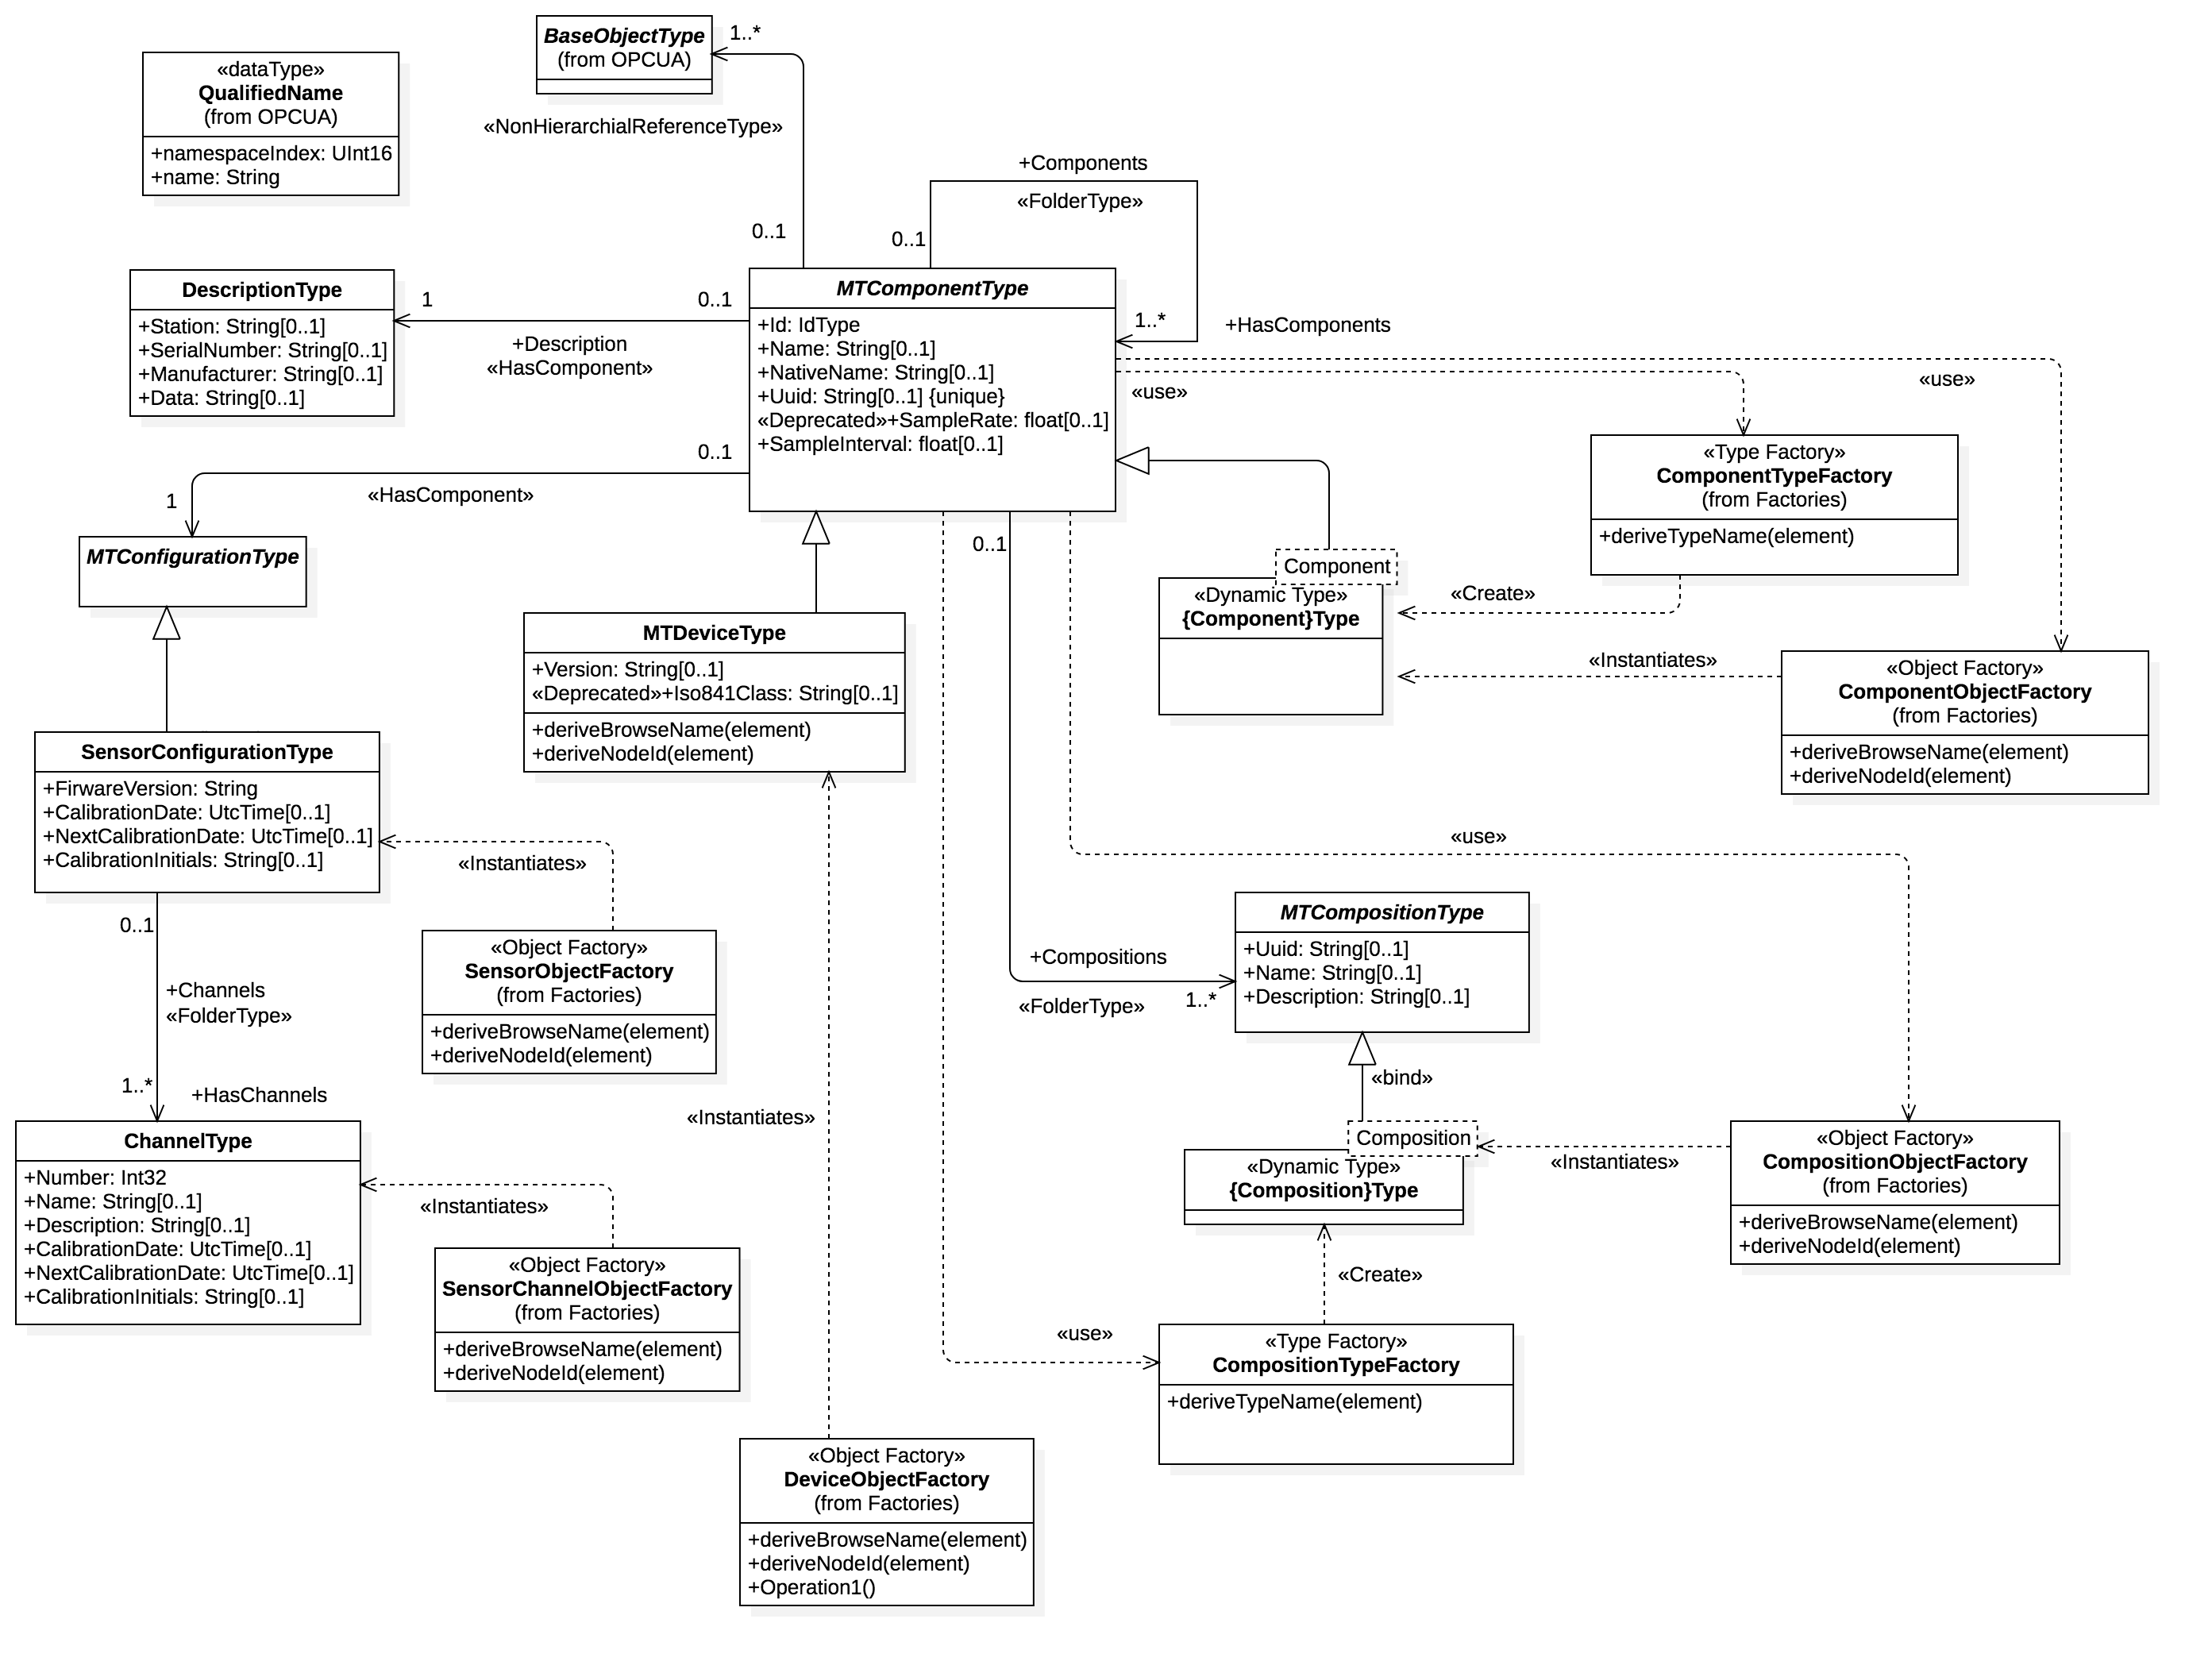
\includegraphics[width=1.0\textwidth]{./diagrams/Components.png}
  \caption{Components Diagram}
  \label{fig:Components}
\end{figure}

\FloatBarrier


The \texttt{Components} documents the Component models and the owned objects.

\subsubsection{Defintion of \texttt{ ChannelType}} \label{type:ChannelType}

\FloatBarrier

An MTConnect \texttt{Channel} is a single data stream associated with a sensor. Each stream
of data can be calibrated separately and allows for the specification of the meta information
and descriptive information. The only required property of the \texttt{Channel} is the number
which is the unique identifier.

The channels will be created by the \texttt{SensorChannelObjectFactory} that composes the \texttt{BrowseName} 
and the \texttt{NodeId} for each object. (See \ref{type:SensorChannelObjectFactory}).

\begin{table}[ht]
\centering 
  \caption{\texttt{ChannelType} Definition}
  \label{table:ChannelType}
\fontsize{9pt}{11pt}\selectfont
\tabulinesep=3pt
\begin{tabu} to 6in {|l|l|l|l|l|l|} \everyrow{\hline}
\hline
\rowfont\bfseries {Attribute} & \multicolumn{5}{|l|}{Value} \\
\tabucline[1.5pt]{}
BrowseName & \multicolumn{5}{|l|}{ChannelType} \\
IsAbstract & \multicolumn{5}{|l|}{False} \\
\tabucline[1.5pt]{}
\rowfont \bfseries References & NodeClass & BrowseName & DataType & TypeDefinition & {Modeling Rule} \\
\multicolumn{6}{|l|}{Subtype of \texttt{BaseObjectType} (See OPC UA Part 5 Documentation)} \\
HasProperty & Variable & Number &  Int32 & PropertyType & Mandatory \\
HasProperty & Variable & Name &  String & PropertyType & Optional \\
HasProperty & Variable & MTDescription &  String & PropertyType & Optional \\
HasProperty & Variable & CalibrationDate &  UtcTime & PropertyType & Optional \\
HasProperty & Variable & NextCalibrationDate &  UtcTime & PropertyType & Optional \\
HasProperty & Variable & CalibrationInitials &  String & PropertyType & Optional \\
\end{tabu}
\end{table} 


\FloatBarrier
\subsubsection{Defintion of \texttt{ CompositionFolderType}} \label{type:CompositionFolderType}

\FloatBarrier

The compositions folder type is organizes the component's composition objects. It will 
only accept objects that are of sub-types of \texttt{MTCompositionType}.

\begin{table}[ht]
\centering 
  \caption{\texttt{CompositionFolderType} Definition}
  \label{table:CompositionFolderType}
\fontsize{9pt}{11pt}\selectfont
\tabulinesep=3pt
\begin{tabu} to 6in {|l|l|l|l|l|l|} \everyrow{\hline}
\hline
\rowfont\bfseries {Attribute} & \multicolumn{5}{|l|}{Value} \\
\tabucline[1.5pt]{}
BrowseName & \multicolumn{5}{|l|}{CompositionFolderType} \\
IsAbstract & \multicolumn{5}{|l|}{False} \\
\tabucline[1.5pt]{}
\rowfont \bfseries References & NodeClass & BrowseName & DataType & TypeDefinition & {Modeling Rule} \\
\multicolumn{6}{|l|}{Subtype of \texttt{FolderType} (See OPC UA Part 5 Documentation)} \\
Organizes & Object & Compositions &  MTCompositionType & Organizes & Optional \\
\end{tabu}
\end{table} 


\FloatBarrier
\subsubsection{Defintion of \texttt{ DescriptionType}} \label{type:DescriptionType}

\FloatBarrier

The description provides some general information about the 
manufacture and serial number of the component. In the XML, the \texttt{CDATA} is freeform 
text that is represented in the \texttt{Data} Property of the Description Object. The description is 
related to the component with the OPC/UA \texttt{HasComponent} relationship.

\begin{table}[ht]
\centering 
  \caption{\texttt{DescriptionType} Definition}
  \label{table:DescriptionType}
\fontsize{9pt}{11pt}\selectfont
\tabulinesep=3pt
\begin{tabu} to 6in {|l|l|l|l|l|l|} \everyrow{\hline}
\hline
\rowfont\bfseries {Attribute} & \multicolumn{5}{|l|}{Value} \\
\tabucline[1.5pt]{}
BrowseName & \multicolumn{5}{|l|}{DescriptionType} \\
IsAbstract & \multicolumn{5}{|l|}{False} \\
\tabucline[1.5pt]{}
\rowfont \bfseries References & NodeClass & BrowseName & DataType & TypeDefinition & {Modeling Rule} \\
\multicolumn{6}{|l|}{Subtype of \texttt{BaseObjectType} (See OPC UA Part 5 Documentation)} \\
HasProperty & Variable & Station &  String & PropertyType & Optional \\
HasProperty & Variable & SerialNumber &  String & PropertyType & Optional \\
HasProperty & Variable & Manufacturer &  String & PropertyType & Optional \\
HasProperty & Variable & Data &  String & PropertyType & Optional \\
\end{tabu}
\end{table} 


\paragraph{Operations}
\begin{itemize}
  \item \texttt{deriveBrowseName(element)}\\
    Specification:
   \indent \begin{lstlisting}
"Description"
\end{lstlisting}

  \item \texttt{deriveNodeId(element)}\\
    Specification:
   \indent \begin{lstlisting}
concat(self.parent.NodeId, BrowseName)
\end{lstlisting}

\end{itemize}
\FloatBarrier
\subsubsection{Defintion of \texttt{ MTComponentFolderType}} \label{type:MTComponentFolderType}

\FloatBarrier



\begin{table}[ht]
\centering 
  \caption{\texttt{MTComponentFolderType} Definition}
  \label{table:MTComponentFolderType}
\fontsize{9pt}{11pt}\selectfont
\tabulinesep=3pt
\begin{tabu} to 6in {|l|l|l|l|l|l|} \everyrow{\hline}
\hline
\rowfont\bfseries {Attribute} & \multicolumn{5}{|l|}{Value} \\
\tabucline[1.5pt]{}
BrowseName & \multicolumn{5}{|l|}{MTComponentFolderType} \\
IsAbstract & \multicolumn{5}{|l|}{False} \\
\tabucline[1.5pt]{}
\rowfont \bfseries References & NodeClass & BrowseName & DataType & TypeDefinition & {Modeling Rule} \\
\multicolumn{6}{|l|}{Subtype of \texttt{FolderType} (See OPC UA Part 5 Documentation)} \\
Organizes & Object & Components &  MTComponentType & Organizes & Optional \\
\end{tabu}
\end{table} 


\FloatBarrier
\subsubsection{Defintion of \texttt{ MTComponentType}} \label{type:MTComponentType}

\FloatBarrier

\begin{figure}[ht]
  \centering
    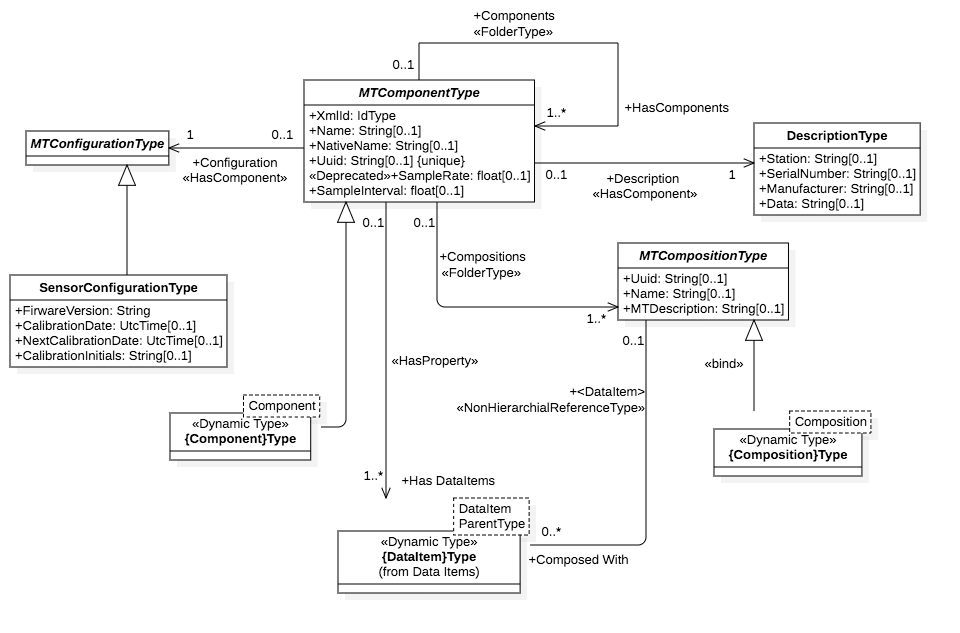
\includegraphics[width=1.0\textwidth]{./diagrams/MTComponentType.png}
  \caption{MTComponentType Diagram}
  \label{fig:MTComponentType}
\end{figure}

\FloatBarrier


The base Component Type from which all MTConnect Components are derived. The 
component type factory is used to create the specific OPC/UA Types as subtypes of the 
MTConnect \texttt{MTComponentType}. The component types will be created once for all Component objects 
of that type based on the \texttt{QName} of the MTConnect XML element. 

The object factory will instantiate the Component Objects and insert them into the Components 
folder with a browse name of the Component QName and the \texttt{name} element if specified surrounded 
by square brackets, \texttt{[]}. For example if the MTConnect Element is:

\texttt{<Linear name='X'>...</...>}

The OPC/UA Object with browse name \texttt{Linear[X]} will be created with the HasTypeDefinition 
referencing the \texttt{Linear} OPC/UA type. 

The meta data for the component and its relationships are static. The dynamic data will be 
represented using the \cite{UAPart8}.



\begin{table}[ht]
\centering 
  \caption{\texttt{MTComponentType} Definition}
  \label{table:MTComponentType}
\fontsize{9pt}{11pt}\selectfont
\tabulinesep=3pt
\begin{tabu} to 6in {|l|l|l|l|l|l|} \everyrow{\hline}
\hline
\rowfont\bfseries {Attribute} & \multicolumn{5}{|l|}{Value} \\
\tabucline[1.5pt]{}
BrowseName & \multicolumn{5}{|l|}{MTComponentType} \\
IsAbstract & \multicolumn{5}{|l|}{True} \\
\tabucline[1.5pt]{}
\rowfont \bfseries References & NodeClass & BrowseName & DataType & TypeDefinition & {Modeling Rule} \\
HasSubtype & ObjectType & MTDeviceType & \multicolumn{3}{|l|}{See section \ref{type:MTDeviceType}} \\
HasSubtype & ObjectType & \{Component\}Type & \multicolumn{3}{|l|}{See section \ref{type:{Component}Type}} \\
HasProperty & Variable & XmlId &  IdType & PropertyType & Mandatory \\
HasProperty & Variable & Name &  String & PropertyType & Optional \\
HasProperty & Variable & NativeName &  String & PropertyType & Optional \\
HasProperty & Variable & Uuid &  String & PropertyType & Optional \\
HasProperty & Variable & SampleRate &  float & PropertyType & Optional \\
HasProperty & Variable & SampleInterval &  float & PropertyType & Optional \\
HasComponent & Object & Description &   & DescriptionType & Optional \\
HasComponent & Object & Configuration &   & MTConfigurationType & Optional \\
HasMTReferenceType & Object & <Dynamic> &  BaseObjectType & <Dynamic> & Optional \\
HasProperty & Variable & <Dynamic> &  MTEnumeratedEventType & PropertyType & Optional \\
HasProperty & Variable & <Dynamic> &  MTNumericEventType & PropertyType & Optional \\
HasProperty & Variable & <Dynamic> &  MTStringEventType & PropertyType & Optional \\
HasProperty & Variable & <Dynamic> &  MTSampleType & PropertyType & Mandatory \\
HasProperty & Variable & <Dynamic> &  MTMessageType & PropertyType & Optional \\
HasProperty & Variable & <Dynamic> &  AssetEventType & PropertyType & Optional \\
\end{tabu}
\end{table} 


\paragraph{Dependency on DataItemObjectFactory}

This class relates to \texttt{DataItemObjectFactory} (See section \ref{type:DataItemObjectFactory}) for a(n) \texttt{use} relationship.

\paragraph{Dependency on CompositionObjectFactory}

This class relates to \texttt{CompositionObjectFactory} (See section \ref{type:CompositionObjectFactory}) for a(n) \texttt{use} relationship.

\paragraph{Dependency on CompositionTypeFactory}

This class relates to \texttt{CompositionTypeFactory} (See section \ref{type:CompositionTypeFactory}) for a(n) \texttt{use} relationship.

\FloatBarrier
\subsubsection{Defintion of \texttt{ MTDeviceType}} \label{type:MTDeviceType}

\FloatBarrier

The MTDevice is a special type whose object will be the root of the device graph. The Device uses the component type factory and the component object factories to create each of the first level components. 

The compositions, relationships, and data items are then recursively created as one descends the MTConnect information model.

\begin{table}[ht]
\centering 
  \caption{\texttt{MTDeviceType} Definition}
  \label{table:MTDeviceType}
\fontsize{9pt}{11pt}\selectfont
\tabulinesep=3pt
\begin{tabu} to 6in {|l|l|l|l|l|l|} \everyrow{\hline}
\hline
\rowfont\bfseries {Attribute} & \multicolumn{5}{|l|}{Value} \\
\tabucline[1.5pt]{}
BrowseName & \multicolumn{5}{|l|}{MTDeviceType} \\
IsAbstract & \multicolumn{5}{|l|}{False} \\
\tabucline[1.5pt]{}
\rowfont \bfseries References & NodeClass & BrowseName & DataType & TypeDefinition & {Modeling Rule} \\
\multicolumn{6}{|l|}{Subtype of \texttt{MTComponentType} (See section \ref{type:MTComponentType})} \\
HasProperty & Variable & Version &  String & PropertyType & Optional \\
HasProperty & Variable & Iso841Class &  String & PropertyType & Optional \\
\end{tabu}
\end{table} 


\paragraph{Constraints}
\begin{itemize}
\item Constraint \texttt{uuid_not_empty}: 
   \indent \begin{lstlisting}
uuid->notEmpty()
\end{lstlisting}
Documentation: The  UUID SHALL be provided.

\end{itemize}
\begin{itemize}
\item Constraint \texttt{name_not_empty}: 
   \indent \begin{lstlisting}
name->notEmpty()
\end{lstlisting}
Documentation: The name of the Device SHALL be given.

\end{itemize}
\paragraph{Dependency on ComponentTypeFactory}

This class relates to \texttt{ComponentTypeFactory} (See section \ref{type:ComponentTypeFactory}) for a(n) \texttt{use} relationship.

\paragraph{Dependency on ComponentObjectFactory}

This class relates to \texttt{ComponentObjectFactory} (See section \ref{type:ComponentObjectFactory}) for a(n) \texttt{use} relationship.

\FloatBarrier
\subsubsection{Defintion of \texttt{<<Dynamic Type>> \{Component\}Type}} \label{type:{Component}Type}

\FloatBarrier

This is a dynamic type that will be created at the time the model is created. The 
\texttt{\{Component\}} placeholder will be supplied by the \texttt{ComponentTypeFactory} 
(\ref{type:ComponentTypeFactory}) that will create the type as a sub-type of the 
\texttt{MTComponentType}.

The name will be created using the \texttt{QName} of the MTConnect \texttt{Component} element.
More information on the MTConnect Components can be found in MTConnect Part 2 \cite{MTCPart2}.

\begin{table}[ht]
\centering 
  \caption{\texttt{\{Component\}Type} Definition}
  \label{table:{Component}Type}
\fontsize{9pt}{11pt}\selectfont
\tabulinesep=3pt
\begin{tabu} to 6in {|l|l|l|l|l|l|} \everyrow{\hline}
\hline
\rowfont\bfseries {Attribute} & \multicolumn{5}{|l|}{Value} \\
\tabucline[1.5pt]{}
BrowseName & \multicolumn{5}{|l|}{{Component}Type} \\
IsAbstract & \multicolumn{5}{|l|}{False} \\
\tabucline[1.5pt]{}
\rowfont \bfseries References & NodeClass & BrowseName & DataType & TypeDefinition & {Modeling Rule} \\
\multicolumn{6}{|l|}{Subtype of \texttt{MTComponentType} (See section \ref{type:MTComponentType})} \\
\end{tabu}
\end{table} 


\FloatBarrier
\subsubsection{Defintion of \texttt{ MTCompositionType}} \label{type:MTCompositionType}

\FloatBarrier

The \texttt{MTCompositionType} is the abstract supertype of the dynamically generated
composition types based on the attribute \texttt{type} of the \texttt{Composition} element
of the MTConnect \texttt{Component}. The \texttt{Composition} is then related to the 
DataItems that reference the \texttt{Composition}'s id in their \texttt{compositionId} 
attribute. 

The data items are added to the relationship where the \texttt{DataItem} to \texttt{Composition} 
relationship is represented by the \texttt{BrowseName} Composition property of the data item.
The data items are added to the \texttt{Composition} by their browse names.

\begin{table}[ht]
\centering 
  \caption{\texttt{MTCompositionType} Definition}
  \label{table:MTCompositionType}
\fontsize{9pt}{11pt}\selectfont
\tabulinesep=3pt
\begin{tabu} to 6in {|l|l|l|l|l|l|} \everyrow{\hline}
\hline
\rowfont\bfseries {Attribute} & \multicolumn{5}{|l|}{Value} \\
\tabucline[1.5pt]{}
BrowseName & \multicolumn{5}{|l|}{MTCompositionType} \\
IsAbstract & \multicolumn{5}{|l|}{True} \\
\tabucline[1.5pt]{}
\rowfont \bfseries References & NodeClass & BrowseName & DataType & TypeDefinition & {Modeling Rule} \\
\multicolumn{6}{|l|}{Subtype of \texttt{BaseObjectType} (See OPC UA Part 5 Documentation)} \\
HasSubtype & ObjectType & \{Composition\}Type & \multicolumn{3}{|l|}{See section \ref{type:{Composition}Type}} \\
HasProperty & Variable & Uuid &  String & PropertyType & Optional \\
HasProperty & Variable & Name &  String & PropertyType & Optional \\
HasProperty & Variable & MTDescription &  String & PropertyType & Optional \\
\end{tabu}
\end{table} 


\FloatBarrier
\subsubsection{Defintion of \texttt{<<Dynamic Type>> \{Composition\}Type}} \label{type:{Composition}Type}

\FloatBarrier

This is a dynamic type that will be created at the time the model is created. The 
\texttt{\{Composition\}} placeholder will be supplied by the \texttt{CompositionTypeFactory} 
(\ref{type:CompositionTypeFactory}) that will create the type as a sub-type of the 
\texttt{MTCompositionType}.

The name will be created using the PascalCase of the \texttt{type} attribute
of the MTConnect \texttt{Composition} element. More information on the MTConnect
Composition can be found in MTConnect Part 2 \cite{MTCPart2}.

\begin{table}[ht]
\centering 
  \caption{\texttt{\{Composition\}Type} Definition}
  \label{table:{Composition}Type}
\fontsize{9pt}{11pt}\selectfont
\tabulinesep=3pt
\begin{tabu} to 6in {|l|l|l|l|l|l|} \everyrow{\hline}
\hline
\rowfont\bfseries {Attribute} & \multicolumn{5}{|l|}{Value} \\
\tabucline[1.5pt]{}
BrowseName & \multicolumn{5}{|l|}{{Composition}Type} \\
IsAbstract & \multicolumn{5}{|l|}{False} \\
\tabucline[1.5pt]{}
\rowfont \bfseries References & NodeClass & BrowseName & DataType & TypeDefinition & {Modeling Rule} \\
\multicolumn{6}{|l|}{Subtype of \texttt{MTCompositionType} (See section \ref{type:MTCompositionType})} \\
\end{tabu}
\end{table} 


\FloatBarrier
\subsubsection{Defintion of \texttt{ MTConfigurationType}} \label{type:MTConfigurationType}

\FloatBarrier

The abstract \texttt{MTConfigurationType} currently has only one sub-type, \\
\texttt{SensorConfigurationType} (see 
\ref{type:SensorConfigurationType}). In the future, the configurations will also contain component 
and device configuration information as sub-types. 

\begin{table}[ht]
\centering 
  \caption{\texttt{MTConfigurationType} Definition}
  \label{table:MTConfigurationType}
\fontsize{9pt}{11pt}\selectfont
\tabulinesep=3pt
\begin{tabu} to 6in {|l|l|l|l|l|l|} \everyrow{\hline}
\hline
\rowfont\bfseries {Attribute} & \multicolumn{5}{|l|}{Value} \\
\tabucline[1.5pt]{}
BrowseName & \multicolumn{5}{|l|}{MTConfigurationType} \\
IsAbstract & \multicolumn{5}{|l|}{True} \\
\tabucline[1.5pt]{}
\rowfont \bfseries References & NodeClass & BrowseName & DataType & TypeDefinition & {Modeling Rule} \\
\multicolumn{6}{|l|}{Subtype of \texttt{BaseObjectType} (See OPC UA Part 5 Documentation)} \\
HasSubtype & ObjectType & SensorConfigurationType & \multicolumn{3}{|l|}{See section \ref{type:SensorConfigurationType}} \\
\end{tabu}
\end{table} 


\FloatBarrier
\subsubsection{Defintion of \texttt{ SensorConfigurationType}} \label{type:SensorConfigurationType}

\FloatBarrier

The \texttt{SensorConfiguration} abstraction provides information required for maintenance and support of a sensor element(s).

The SensorConfiguration browse name will be created as an Object relationship with the parent component.

\begin{table}[ht]
\centering 
  \caption{\texttt{SensorConfigurationType} Definition}
  \label{table:SensorConfigurationType}
\fontsize{9pt}{11pt}\selectfont
\tabulinesep=3pt
\begin{tabu} to 6in {|l|l|l|l|l|l|} \everyrow{\hline}
\hline
\rowfont\bfseries {Attribute} & \multicolumn{5}{|l|}{Value} \\
\tabucline[1.5pt]{}
BrowseName & \multicolumn{5}{|l|}{SensorConfigurationType} \\
IsAbstract & \multicolumn{5}{|l|}{False} \\
\tabucline[1.5pt]{}
\rowfont \bfseries References & NodeClass & BrowseName & DataType & TypeDefinition & {Modeling Rule} \\
\multicolumn{6}{|l|}{Subtype of \texttt{MTConfigurationType} (See section \ref{type:MTConfigurationType})} \\
HasProperty & Variable & FirwareVersion &  String & PropertyType & Mandatory \\
HasProperty & Variable & CalibrationDate &  UtcTime & PropertyType & Optional \\
HasProperty & Variable & NextCalibrationDate &  UtcTime & PropertyType & Optional \\
HasProperty & Variable & CalibrationInitials &  String & PropertyType & Optional \\
HasChannels & Object & Channels &  ChannelType & HasChannels & Optional \\
\end{tabu}
\end{table} 


\FloatBarrier
\subsection{Data Items} \label{model:DataItems}

\begin{figure}[ht]
  \centering
    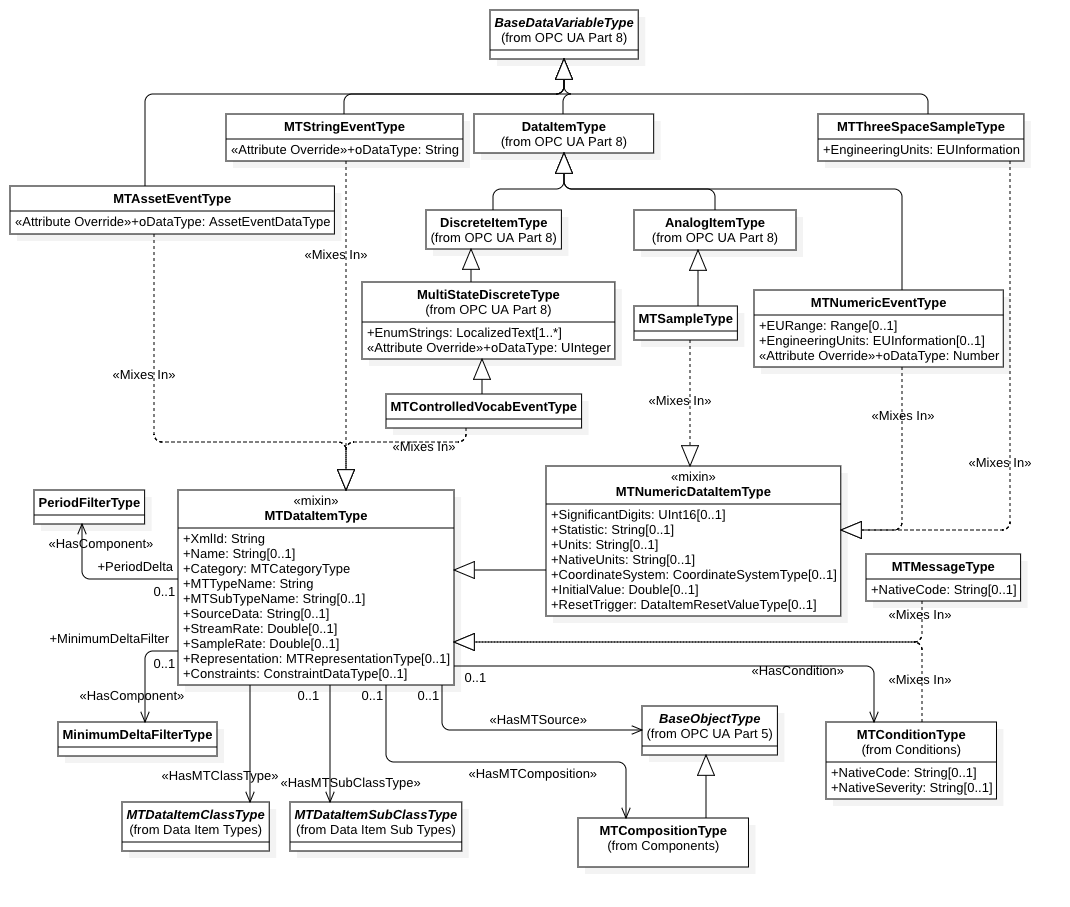
\includegraphics[width=1.0\textwidth]{./diagrams/DataItems.png}
  \caption{Data Items Diagram}
  \label{fig:DataItems}
\end{figure}

\FloatBarrier

\subsubsection{Defintion of \texttt{ AssetEventType}} \label{type:AssetEventType}

\FloatBarrier

The asset events have an additional attribute regarding the asset change or removal identifier
and the type of asset that is being reported.


\begin{table}[ht]
\centering 
  \caption{\texttt{AssetEventType} Definition}
  \label{table:AssetEventType}
\fontsize{9pt}{11pt}\selectfont
\tabulinesep=3pt
\begin{tabu} to 6in {|l|l|l|l|l|l|} \everyrow{\hline}
\hline
\rowfont\bfseries {Attribute} & \multicolumn{5}{|l|}{Value} \\
\tabucline[1.5pt]{}
BrowseName & \multicolumn{5}{|l|}{AssetEventType} \\
IsAbstract & \multicolumn{5}{|l|}{False} \\
ValueRank & \multicolumn{5}{|l|}{-1} \\
DataType & \multicolumn{5}{|l|}{AssetEventDataType} \\
\tabucline[1.5pt]{}
\rowfont \bfseries References & NodeClass & BrowseName & DataType & TypeDefinition & {Modeling Rule} \\
\multicolumn{6}{|l|}{Subtype of \texttt{BaseDataVariableType} (See OPC UA Part 8 Documentation)} \\
HasProperty & Variable & Category &  MTCategoryType & PropertyType & Mandatory \\
HasProperty & Variable & MTClassName &  String & PropertyType & Mandatory \\
HasProperty & Variable & MTSubTypeName &  String & PropertyType & Optional \\
HasProperty & Variable & SourceName &  String & PropertyType & Optional \\
HasProperty & Variable & StreamRate &  Double & PropertyType & Optional \\
HasProperty & Variable & SampleRate &  Double & PropertyType & Optional \\
HasProperty & Variable & Representation &  RepresentationType & PropertyType & Optional \\
HasMTClassType & Object & <Dynamic> &  MTDataItemClassType & <Dynamic> & Mandatory \\
HasMTSubClassType & Object & <Dynamic> &  MTDataItemSubClassType & <Dynamic> & Optional \\
HasComponent & Object & MinimumDeltaFilter &  MinimumDeltaFilterType & HasComponent & Optional \\
HasComponent & Object & PeriodDelta &  PeriodFilterType & HasComponent & Optional \\
HasMTComposition & Object & <Dynamic> &  MTCompositionType & <Dynamic> & Optional \\
\end{tabu}
\end{table} 


\paragraph{Mixes in \texttt{MTDataItemType}} (See section \ref{type:MTDataItemType})
\FloatBarrier
\subsubsection{Defintion of \texttt{<<mixin>> MTDataItemType}} \label{type:MTDataItemType}

\FloatBarrier

The data item mixin will inject the properties and the methods into the related 
classes. This facility is similar to the Ruby module mixin or the Scala traits.

\begin{table}[ht]
\centering 
  \caption{\texttt{MTDataItemType} Definition}
  \label{table:MTDataItemType}
\fontsize{9pt}{11pt}\selectfont
\tabulinesep=3pt
\begin{tabu} to 6in {|l|l|l|l|l|l|} \everyrow{\hline}
\hline
\rowfont\bfseries {Attribute} & \multicolumn{5}{|l|}{Value} \\
\tabucline[1.5pt]{}
BrowseName & \multicolumn{5}{|l|}{MTDataItemType} \\
IsAbstract & \multicolumn{5}{|l|}{False} \\
\tabucline[1.5pt]{}
\rowfont \bfseries References & NodeClass & BrowseName & DataType & TypeDefinition & {Modeling Rule} \\
HasSubtype & ObjectType & MTNumericDataItemType & \multicolumn{3}{|l|}{See section \ref{type:MTNumericDataItemType}} \\
HasProperty & Variable & Category &  MTCategoryType & PropertyType & Mandatory \\
HasProperty & Variable & MTClassName &  String & PropertyType & Mandatory \\
HasProperty & Variable & MTSubTypeName &  String & PropertyType & Optional \\
HasProperty & Variable & SourceName &  String & PropertyType & Optional \\
HasProperty & Variable & StreamRate &  Double & PropertyType & Optional \\
HasProperty & Variable & SampleRate &  Double & PropertyType & Optional \\
HasProperty & Variable & Representation &  RepresentationType & PropertyType & Optional \\
HasMTClassType & Object & <Dynamic> &  MTDataItemClassType & <Dynamic> & Mandatory \\
HasMTSubClassType & Object & <Dynamic> &  MTDataItemSubClassType & <Dynamic> & Optional \\
HasComponent & Object & MinimumDeltaFilter &  MinimumDeltaFilterType & HasComponent & Optional \\
HasComponent & Object & PeriodDelta &  PeriodFilterType & HasComponent & Optional \\
HasMTComposition & Object & <Dynamic> &  MTCompositionType & <Dynamic> & Optional \\
\end{tabu}
\end{table} 


\paragraph{Operations}
\begin{itemize}
  \item \texttt{deriveSourceName(element)}\\
    Specification:
   \indent \begin{lstlisting}
self.Source.CDATA
\end{lstlisting}

    Documentation: Derive the source name from the Source element CDATA. This will represent the alternative long name for the data item's source.

  \item \texttt{getStatusCode()}
    Documentation: The OPC/UA status code will be created using the following process:

\begin{itemize}
  \item If the value of the data item is \texttt{UNAVAILABLE} a status code of \texttt{Uncertain_NoCommunicationLastUsable}
  \item When a reset trigger is specified, new \texttt{Good_} status codes will be created. See \texttt{ResetTrigger} enumeration.
\end{itemize}

\end{itemize}
\FloatBarrier
\subsubsection{Defintion of \texttt{<<mixin>> MTNumericDataItemType}} \label{type:MTNumericDataItemType}

\FloatBarrier

These are the additional attributes that are relevent to numeric data items. 
The factory will evaluate these values and will set the engineering units and the 
range associated with the parent entity.

\begin{table}[ht]
\centering 
  \caption{\texttt{MTNumericDataItemType} Definition}
  \label{table:MTNumericDataItemType}
\fontsize{9pt}{11pt}\selectfont
\tabulinesep=3pt
\begin{tabu} to 6in {|l|l|l|l|l|l|} \everyrow{\hline}
\hline
\rowfont\bfseries {Attribute} & \multicolumn{5}{|l|}{Value} \\
\tabucline[1.5pt]{}
BrowseName & \multicolumn{5}{|l|}{MTNumericDataItemType} \\
IsAbstract & \multicolumn{5}{|l|}{False} \\
\tabucline[1.5pt]{}
\rowfont \bfseries References & NodeClass & BrowseName & DataType & TypeDefinition & {Modeling Rule} \\
\multicolumn{6}{|l|}{Subtype of \texttt{MTDataItemType} (See section \ref{type:MTDataItemType})} \\
HasProperty & Variable & SignificantDigits &  UInt16 & PropertyType & Optional \\
HasProperty & Variable & Statistic &  MTStatisticType & PropertyType & Optional \\
HasProperty & Variable & Units &  MTUnits & PropertyType & Optional \\
HasProperty & Variable & NativeUnits &  MTNativeUnitsType & PropertyType & Optional \\
HasProperty & Variable & CoordinateSystem &  MTCoordinateSystemType & PropertyType & Optional \\
HasProperty & Variable & InitialValue &  Double & PropertyType & Optional \\
HasProperty & Variable & ResetTrigger &  DataItemResetValueType & PropertyType & Optional \\
HasProperty & Variable & Nominal &  Double & PropertyType & Optional \\
\end{tabu}
\end{table} 


\paragraph{Operations}
\begin{itemize}
  \item \texttt{deriveEngineeringUnits(units)}\\
    Specification:
   \indent \begin{lstlisting}
EngineeringUnits <- self.units
\end{lstlisting}

  \item \texttt{deriveEURange(constraints)}\\
    Specification:
   \indent \begin{lstlisting}
EURange.Low <- self.Constraints.Minimum
EURange.High <- self.Constraints.Maximum
\end{lstlisting}

    Documentation: Uses the MTConnect Constraints element if present to derive the minimum 
and maximum values for the numeric values. This applies to both the Numeric 
Event and the Sample types.

\end{itemize}
\FloatBarrier
\subsubsection{Defintion of \texttt{ MTEnumeratedEventType}} \label{type:MTEnumeratedEventType}

\FloatBarrier

All Data Items with Category \texttt{EVENT} having Controlled Vocabularies (Enumerations) 
will be added as sub-types of this type which is mapped to the OPC/UA MultiStateValueDiscreteType. 
Otherwise, either \texttt{MTString} or \texttt{MTNumeric} will be used. All subtypes are direct representations of the 
MTConnect equivalent elements that can be found in the \textit{MTConnect Part 3} documents.

\begin{table}[ht]
\centering 
  \caption{\texttt{MTEnumeratedEventType} Definition}
  \label{table:MTEnumeratedEventType}
\fontsize{9pt}{11pt}\selectfont
\tabulinesep=3pt
\begin{tabu} to 6in {|l|l|l|l|l|l|} \everyrow{\hline}
\hline
\rowfont\bfseries {Attribute} & \multicolumn{5}{|l|}{Value} \\
\tabucline[1.5pt]{}
BrowseName & \multicolumn{5}{|l|}{MTEnumeratedEventType} \\
IsAbstract & \multicolumn{5}{|l|}{False} \\
ValueRank & \multicolumn{5}{|l|}{-1} \\
DataType & \multicolumn{5}{|l|}{EnumValuesType} \\
\tabucline[1.5pt]{}
\rowfont \bfseries References & NodeClass & BrowseName & DataType & TypeDefinition & {Modeling Rule} \\
\multicolumn{6}{|l|}{Subtype of \texttt{MultiStateDiscreteType} (See OPC UA Part 8 Documentation)} \\
HasProperty & Variable & Category &  MTCategoryType & PropertyType & Mandatory \\
HasProperty & Variable & MTClassName &  String & PropertyType & Mandatory \\
HasProperty & Variable & MTSubTypeName &  String & PropertyType & Optional \\
HasProperty & Variable & SourceName &  String & PropertyType & Optional \\
HasProperty & Variable & StreamRate &  Double & PropertyType & Optional \\
HasProperty & Variable & SampleRate &  Double & PropertyType & Optional \\
HasProperty & Variable & Representation &  RepresentationType & PropertyType & Optional \\
HasMTClassType & Object & <Dynamic> &  MTDataItemClassType & <Dynamic> & Mandatory \\
HasMTSubClassType & Object & <Dynamic> &  MTDataItemSubClassType & <Dynamic> & Optional \\
HasComponent & Object & MinimumDeltaFilter &  MinimumDeltaFilterType & HasComponent & Optional \\
HasComponent & Object & PeriodDelta &  PeriodFilterType & HasComponent & Optional \\
HasMTComposition & Object & <Dynamic> &  MTCompositionType & <Dynamic> & Optional \\
HasProperty & Variable & ConstrainedDataType &  EnumValuesType & PropertyType & Optional \\
\end{tabu}
\end{table} 


\paragraph{Mixes in \texttt{MTDataItemType}} (See section \ref{type:MTDataItemType})
\FloatBarrier
\subsubsection{Defintion of \texttt{ MTFilterType}} \label{type:MTFilterType}

\FloatBarrier

These features will be subsumed by the OPC/UA client filtering directives. They are included
since they document the MTConnect filtering on the incoming stream of data. The
subtypes will be instantiated by the FilterObjectFactory if they are secified
for this data item. See \ref{type:FilterObjectFactory} for more information.

\begin{table}[ht]
\centering 
  \caption{\texttt{MTFilterType} Definition}
  \label{table:MTFilterType}
\fontsize{9pt}{11pt}\selectfont
\tabulinesep=3pt
\begin{tabu} to 6in {|l|l|l|l|l|l|} \everyrow{\hline}
\hline
\rowfont\bfseries {Attribute} & \multicolumn{5}{|l|}{Value} \\
\tabucline[1.5pt]{}
BrowseName & \multicolumn{5}{|l|}{MTFilterType} \\
IsAbstract & \multicolumn{5}{|l|}{True} \\
\tabucline[1.5pt]{}
\rowfont \bfseries References & NodeClass & BrowseName & DataType & TypeDefinition & {Modeling Rule} \\
HasSubtype & ObjectType & MinimumDeltaFilterType & \multicolumn{3}{|l|}{See section \ref{type:MinimumDeltaFilterType}} \\
HasSubtype & ObjectType & PeriodFilterType & \multicolumn{3}{|l|}{See section \ref{type:PeriodFilterType}} \\
HasProperty & Variable & Value &  float & PropertyType & Mandatory \\
\end{tabu}
\end{table} 


\FloatBarrier
\subsubsection{Defintion of \texttt{ MinimumDeltaFilterType}} \label{type:MinimumDeltaFilterType}

\FloatBarrier

The minimum delta filter will not report data if the change in the value of the
data item is less than the given value in the \texttt{Value} property. 

\begin{table}[ht]
\centering 
  \caption{\texttt{MinimumDeltaFilterType} Definition}
  \label{table:MinimumDeltaFilterType}
\fontsize{9pt}{11pt}\selectfont
\tabulinesep=3pt
\begin{tabu} to 6in {|l|l|l|l|l|l|} \everyrow{\hline}
\hline
\rowfont\bfseries {Attribute} & \multicolumn{5}{|l|}{Value} \\
\tabucline[1.5pt]{}
BrowseName & \multicolumn{5}{|l|}{MinimumDeltaFilterType} \\
IsAbstract & \multicolumn{5}{|l|}{False} \\
\tabucline[1.5pt]{}
\rowfont \bfseries References & NodeClass & BrowseName & DataType & TypeDefinition & {Modeling Rule} \\
\multicolumn{6}{|l|}{Subtype of \texttt{MTFilterType} (See section \ref{type:MTFilterType})} \\
\end{tabu}
\end{table} 


\FloatBarrier
\subsubsection{Defintion of \texttt{ PeriodFilterType}} \label{type:PeriodFilterType}

\FloatBarrier

A period filter sets the minimum number of seconds that must elapse before
a change is reported as given in the \texttt{Value} property.


\begin{table}[ht]
\centering 
  \caption{\texttt{PeriodFilterType} Definition}
  \label{table:PeriodFilterType}
\fontsize{9pt}{11pt}\selectfont
\tabulinesep=3pt
\begin{tabu} to 6in {|l|l|l|l|l|l|} \everyrow{\hline}
\hline
\rowfont\bfseries {Attribute} & \multicolumn{5}{|l|}{Value} \\
\tabucline[1.5pt]{}
BrowseName & \multicolumn{5}{|l|}{PeriodFilterType} \\
IsAbstract & \multicolumn{5}{|l|}{False} \\
\tabucline[1.5pt]{}
\rowfont \bfseries References & NodeClass & BrowseName & DataType & TypeDefinition & {Modeling Rule} \\
\multicolumn{6}{|l|}{Subtype of \texttt{MTFilterType} (See section \ref{type:MTFilterType})} \\
\end{tabu}
\end{table} 


\FloatBarrier
\subsubsection{Defintion of \texttt{ MTMessageType}} \label{type:MTMessageType}

\FloatBarrier

The message type is a special class since it adds another property for the native code. 
In MTConnect the \texttt{nativeCode} attribute will be mapped to this variable 
in the message. The type is currently sub-typed from the OPC UA \texttt{SystemEventType} and 
will be represented as an event. The MTConnect CDATA will be represented in the Event 
\texttt{Message}.


\begin{table}[ht]
\centering 
  \caption{\texttt{MTMessageType} Definition}
  \label{table:MTMessageType}
\fontsize{9pt}{11pt}\selectfont
\tabulinesep=3pt
\begin{tabu} to 6in {|l|l|l|l|l|l|} \everyrow{\hline}
\hline
\rowfont\bfseries {Attribute} & \multicolumn{5}{|l|}{Value} \\
\tabucline[1.5pt]{}
BrowseName & \multicolumn{5}{|l|}{MTMessageType} \\
IsAbstract & \multicolumn{5}{|l|}{False} \\
\tabucline[1.5pt]{}
\rowfont \bfseries References & NodeClass & BrowseName & DataType & TypeDefinition & {Modeling Rule} \\
\multicolumn{6}{|l|}{Subtype of \texttt{SystemEventType} (See OPC UA Part 5 Documentation)} \\
HasProperty & Variable & NativeCode &  String & PropertyType & Optional \\
\end{tabu}
\end{table} 


\FloatBarrier
\subsubsection{Defintion of \texttt{ MTNumericEventType}} \label{type:MTNumericEventType}

\FloatBarrier

All data items with category \texttt{EVENT} and a numeric value. These are usually counters for 
parts and lines. Currently only builtin types that are known to be integers will be
sub-typed from this type. Extended types will be subtyped from the \texttt{MTStringEventType}.

\begin{table}[ht]
\centering 
  \caption{\texttt{MTNumericEventType} Definition}
  \label{table:MTNumericEventType}
\fontsize{9pt}{11pt}\selectfont
\tabulinesep=3pt
\begin{tabu} to 6in {|l|l|l|l|l|l|} \everyrow{\hline}
\hline
\rowfont\bfseries {Attribute} & \multicolumn{5}{|l|}{Value} \\
\tabucline[1.5pt]{}
BrowseName & \multicolumn{5}{|l|}{MTNumericEventType} \\
IsAbstract & \multicolumn{5}{|l|}{False} \\
ValueRank & \multicolumn{5}{|l|}{-1} \\
DataType & \multicolumn{5}{|l|}{Number} \\
\tabucline[1.5pt]{}
\rowfont \bfseries References & NodeClass & BrowseName & DataType & TypeDefinition & {Modeling Rule} \\
\multicolumn{6}{|l|}{Subtype of \texttt{DataItemType} (See OPC UA Part 8 Documentation)} \\
HasProperty & Variable & Category &  MTCategoryType & PropertyType & Mandatory \\
HasProperty & Variable & MTClassName &  String & PropertyType & Mandatory \\
HasProperty & Variable & MTSubTypeName &  String & PropertyType & Optional \\
HasProperty & Variable & SourceName &  String & PropertyType & Optional \\
HasProperty & Variable & StreamRate &  Double & PropertyType & Optional \\
HasProperty & Variable & SampleRate &  Double & PropertyType & Optional \\
HasProperty & Variable & Representation &  RepresentationType & PropertyType & Optional \\
HasMTClassType & Object & <Dynamic> &  MTDataItemClassType & <Dynamic> & Mandatory \\
HasMTSubClassType & Object & <Dynamic> &  MTDataItemSubClassType & <Dynamic> & Optional \\
HasComponent & Object & MinimumDeltaFilter &  MinimumDeltaFilterType & HasComponent & Optional \\
HasComponent & Object & PeriodDelta &  PeriodFilterType & HasComponent & Optional \\
HasMTComposition & Object & <Dynamic> &  MTCompositionType & <Dynamic> & Optional \\
HasProperty & Variable & SignificantDigits &  UInt16 & PropertyType & Optional \\
HasProperty & Variable & Statistic &  MTStatisticType & PropertyType & Optional \\
HasProperty & Variable & Units &  MTUnits & PropertyType & Optional \\
HasProperty & Variable & NativeUnits &  MTNativeUnitsType & PropertyType & Optional \\
HasProperty & Variable & CoordinateSystem &  MTCoordinateSystemType & PropertyType & Optional \\
HasProperty & Variable & InitialValue &  Double & PropertyType & Optional \\
HasProperty & Variable & ResetTrigger &  DataItemResetValueType & PropertyType & Optional \\
HasProperty & Variable & Nominal &  Double & PropertyType & Optional \\
HasProperty & Variable & EURange &  Range & PropertyType & Optional \\
HasProperty & Variable & EngineeringUnits &  EUInformation & PropertyType & Optional \\
\end{tabu}
\end{table} 


\paragraph{Mixes in \texttt{MTNumericDataItemType}} (See section \ref{type:MTNumericDataItemType})
\FloatBarrier
\subsubsection{Defintion of \texttt{ MTSampleType}} \label{type:MTSampleType}

\FloatBarrier

Data Items with category \texttt{SAMPLE}. The simplest mapping since all these types are 
floating numeric data and comply with the AnalogItemType from OPC/UA Part 8.

\begin{table}[ht]
\centering 
  \caption{\texttt{MTSampleType} Definition}
  \label{table:MTSampleType}
\fontsize{9pt}{11pt}\selectfont
\tabulinesep=3pt
\begin{tabu} to 6in {|l|l|l|l|l|l|} \everyrow{\hline}
\hline
\rowfont\bfseries {Attribute} & \multicolumn{5}{|l|}{Value} \\
\tabucline[1.5pt]{}
BrowseName & \multicolumn{5}{|l|}{MTSampleType} \\
IsAbstract & \multicolumn{5}{|l|}{False} \\
ValueRank & \multicolumn{5}{|l|}{-1} \\
DataType & \multicolumn{5}{|l|}{Number} \\
\tabucline[1.5pt]{}
\rowfont \bfseries References & NodeClass & BrowseName & DataType & TypeDefinition & {Modeling Rule} \\
\multicolumn{6}{|l|}{Subtype of \texttt{AnalogItemType} (See OPC UA Part 8 Documentation)} \\
HasProperty & Variable & Category &  MTCategoryType & PropertyType & Mandatory \\
HasProperty & Variable & MTClassName &  String & PropertyType & Mandatory \\
HasProperty & Variable & MTSubTypeName &  String & PropertyType & Optional \\
HasProperty & Variable & SourceName &  String & PropertyType & Optional \\
HasProperty & Variable & StreamRate &  Double & PropertyType & Optional \\
HasProperty & Variable & SampleRate &  Double & PropertyType & Optional \\
HasProperty & Variable & Representation &  RepresentationType & PropertyType & Optional \\
HasMTClassType & Object & <Dynamic> &  MTDataItemClassType & <Dynamic> & Mandatory \\
HasMTSubClassType & Object & <Dynamic> &  MTDataItemSubClassType & <Dynamic> & Optional \\
HasComponent & Object & MinimumDeltaFilter &  MinimumDeltaFilterType & HasComponent & Optional \\
HasComponent & Object & PeriodDelta &  PeriodFilterType & HasComponent & Optional \\
HasMTComposition & Object & <Dynamic> &  MTCompositionType & <Dynamic> & Optional \\
HasProperty & Variable & SignificantDigits &  UInt16 & PropertyType & Optional \\
HasProperty & Variable & Statistic &  MTStatisticType & PropertyType & Optional \\
HasProperty & Variable & Units &  MTUnits & PropertyType & Optional \\
HasProperty & Variable & NativeUnits &  MTNativeUnitsType & PropertyType & Optional \\
HasProperty & Variable & CoordinateSystem &  MTCoordinateSystemType & PropertyType & Optional \\
HasProperty & Variable & InitialValue &  Double & PropertyType & Optional \\
HasProperty & Variable & ResetTrigger &  DataItemResetValueType & PropertyType & Optional \\
HasProperty & Variable & Nominal &  Double & PropertyType & Optional \\
\end{tabu}
\end{table} 


\paragraph{Mixes in \texttt{MTNumericDataItemType}} (See section \ref{type:MTNumericDataItemType})
\FloatBarrier
\subsubsection{Defintion of \texttt{ MTStringEventType}} \label{type:MTStringEventType}

\FloatBarrier

All data items with category \texttt{EVENT} where the data is freeform text. The data type
will be set to String for all the sub-types. All extended type, regardless of 
controlled vocabularies, will use this base type unless proprietary 
enumerations are added to the nodeset as required by the builtin state
event types inherited from \texttt{MTEnumeratedEventType} (see \ref{type:MTEnumeratedEventType}).

\begin{table}[ht]
\centering 
  \caption{\texttt{MTStringEventType} Definition}
  \label{table:MTStringEventType}
\fontsize{9pt}{11pt}\selectfont
\tabulinesep=3pt
\begin{tabu} to 6in {|l|l|l|l|l|l|} \everyrow{\hline}
\hline
\rowfont\bfseries {Attribute} & \multicolumn{5}{|l|}{Value} \\
\tabucline[1.5pt]{}
BrowseName & \multicolumn{5}{|l|}{MTStringEventType} \\
IsAbstract & \multicolumn{5}{|l|}{False} \\
ValueRank & \multicolumn{5}{|l|}{-1} \\
DataType & \multicolumn{5}{|l|}{String} \\
\tabucline[1.5pt]{}
\rowfont \bfseries References & NodeClass & BrowseName & DataType & TypeDefinition & {Modeling Rule} \\
\multicolumn{6}{|l|}{Subtype of \texttt{BaseDataVariableType} (See OPC UA Part 8 Documentation)} \\
HasProperty & Variable & Category &  MTCategoryType & PropertyType & Mandatory \\
HasProperty & Variable & MTClassName &  String & PropertyType & Mandatory \\
HasProperty & Variable & MTSubTypeName &  String & PropertyType & Optional \\
HasProperty & Variable & SourceName &  String & PropertyType & Optional \\
HasProperty & Variable & StreamRate &  Double & PropertyType & Optional \\
HasProperty & Variable & SampleRate &  Double & PropertyType & Optional \\
HasProperty & Variable & Representation &  RepresentationType & PropertyType & Optional \\
HasMTClassType & Object & <Dynamic> &  MTDataItemClassType & <Dynamic> & Mandatory \\
HasMTSubClassType & Object & <Dynamic> &  MTDataItemSubClassType & <Dynamic> & Optional \\
HasComponent & Object & MinimumDeltaFilter &  MinimumDeltaFilterType & HasComponent & Optional \\
HasComponent & Object & PeriodDelta &  PeriodFilterType & HasComponent & Optional \\
HasMTComposition & Object & <Dynamic> &  MTCompositionType & <Dynamic> & Optional \\
\end{tabu}
\end{table} 


\paragraph{Mixes in \texttt{MTDataItemType}} (See section \ref{type:MTDataItemType})
\FloatBarrier
\subsection{Conditions} \label{model:Conditions}

\begin{figure}[ht]
  \centering
    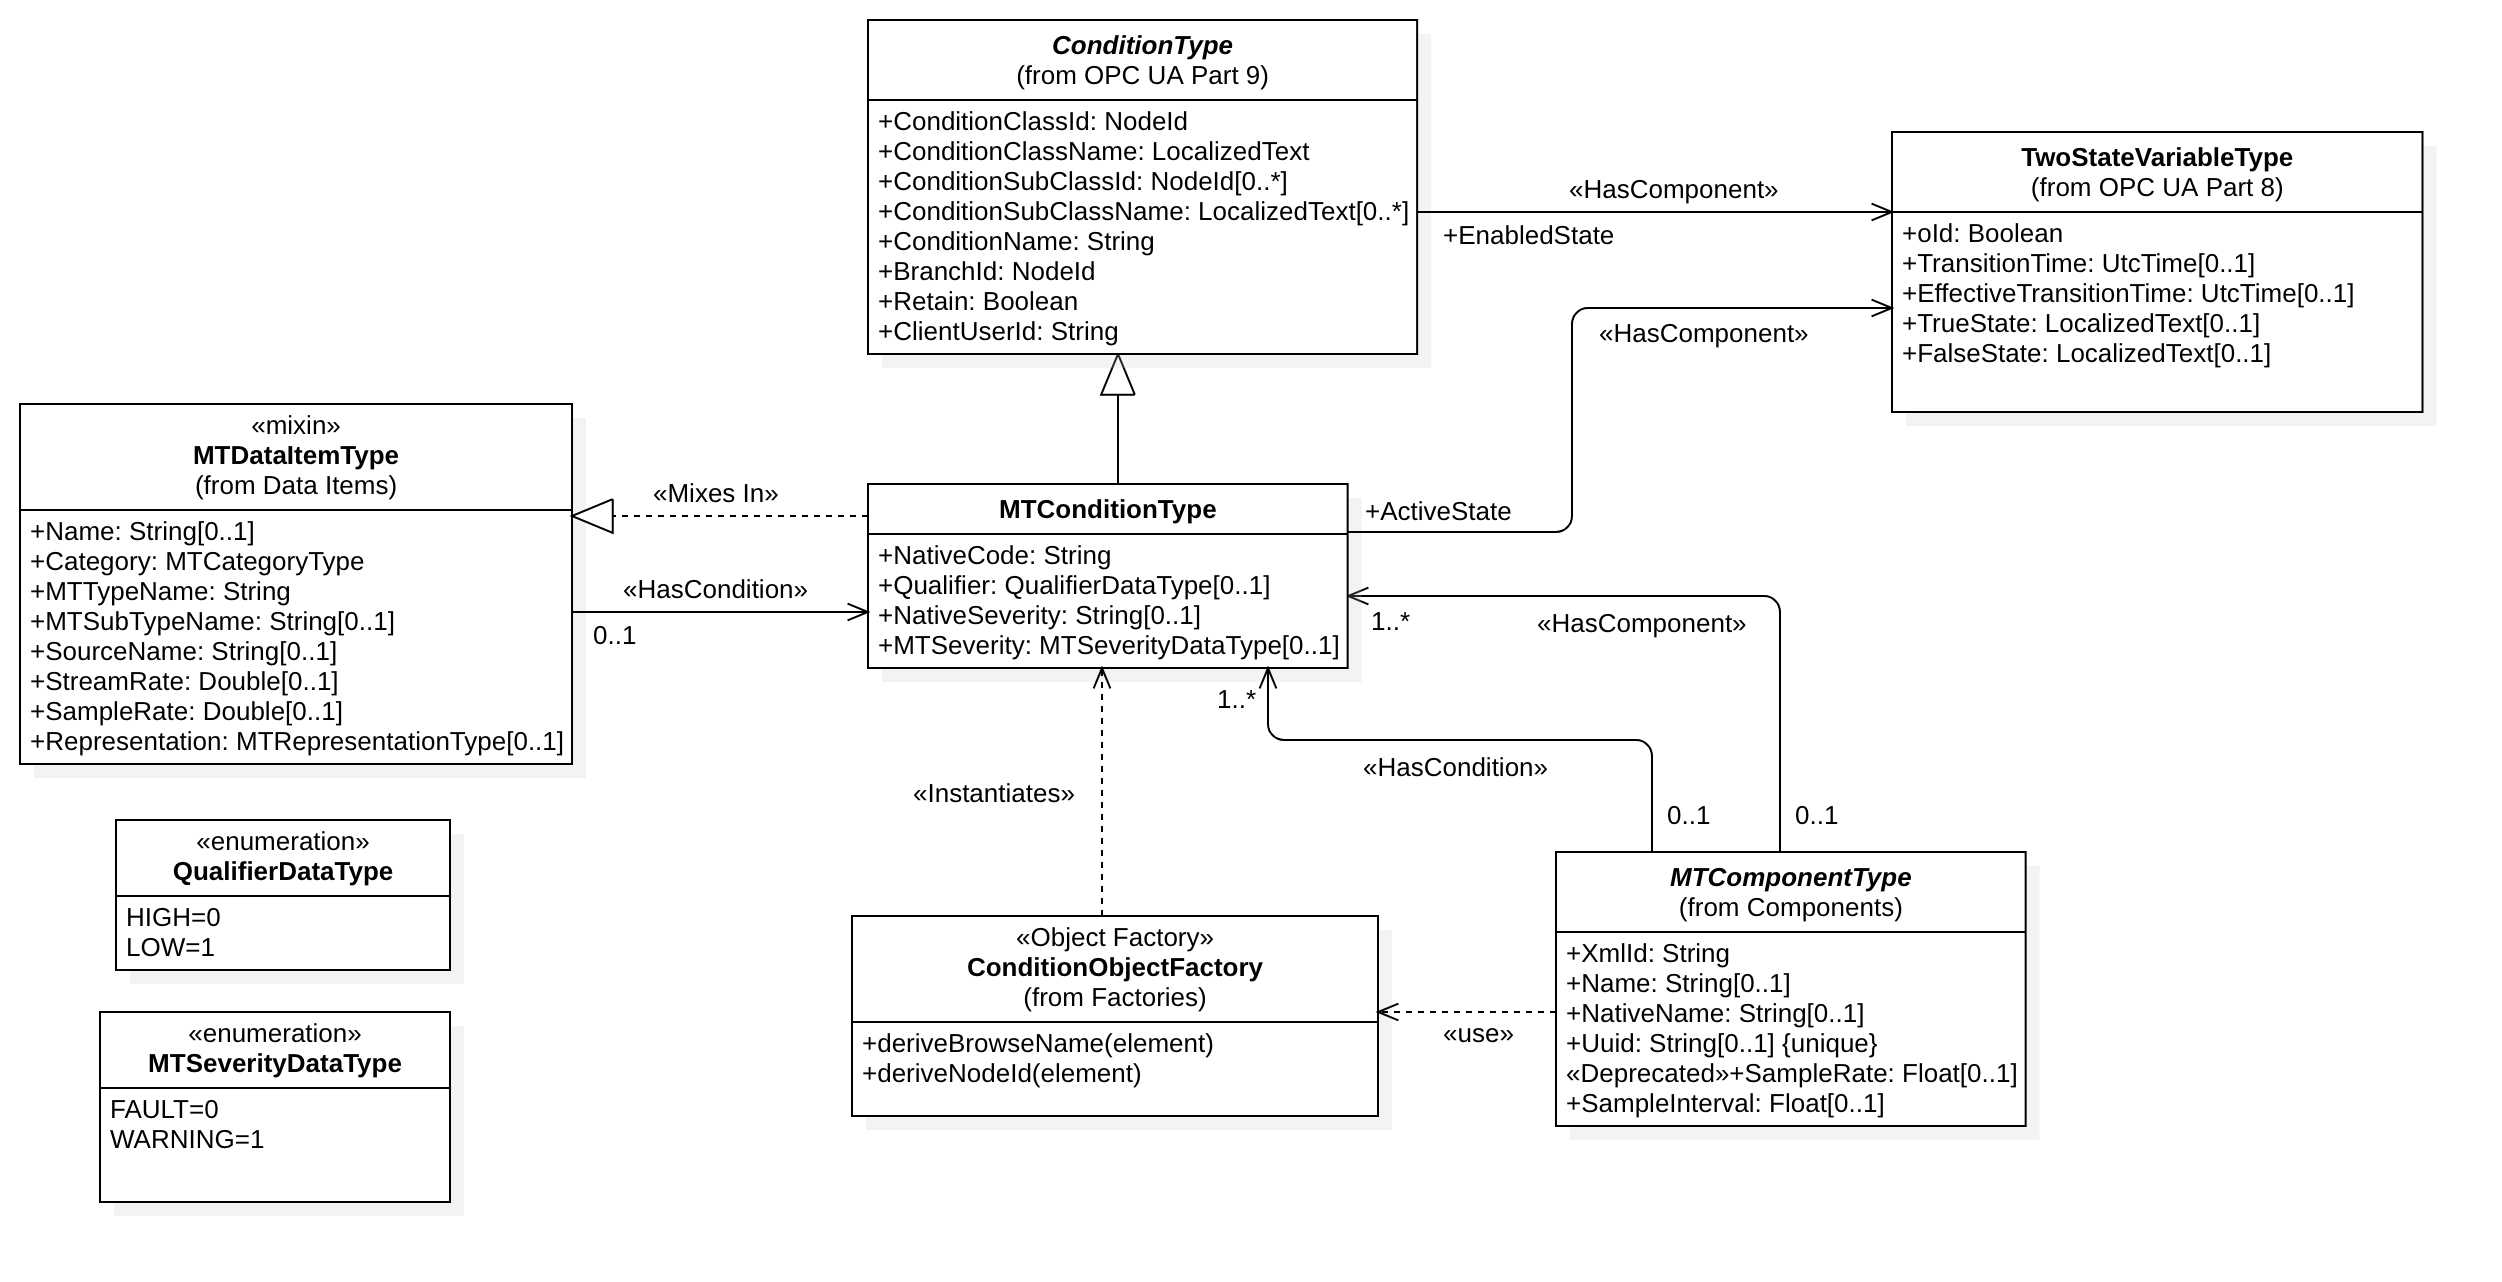
\includegraphics[width=1.0\textwidth]{./diagrams/Conditions.png}
  \caption{Conditions Diagram}
  \label{fig:Conditions}
\end{figure}

\FloatBarrier


The parallel modeling of conditions and alarms in MTConnect and OPC UA represent some
situation where something has been detected that is not expected or outside of the norm. The
documentation for the condition behavior in MTConnect can be found in Section 5.7 and 
5.8 of \cite{MTCPart3}.

The MTConnect Data Item with Category of \texttt{CONDITION} are used to map to the 
OPC UA \texttt{ConditionType} models in \cite{UAPart9}

\subsubsection{Defintion of \texttt{ ConditionFolderType}} \label{type:ConditionFolderType}

\FloatBarrier


The conditions folder type contains all the components \texttt{DataItems} that are
of category \texttt{CONDITION}. See MTConnect Part 1 \cite{MTCPart1} and MTConnect Part 2
\cite{MTCPart2} for a complete discussion of MTConnect Conditions.

\begin{table}[ht]
\centering 
  \caption{\texttt{ConditionFolderType} Definition}
  \label{table:ConditionFolderType}
\fontsize{9pt}{11pt}\selectfont
\tabulinesep=3pt
\begin{tabu} to 6in {|l|l|l|l|l|l|} \everyrow{\hline}
\hline
\rowfont\bfseries {Attribute} & \multicolumn{5}{|l|}{Value} \\
\tabucline[1.5pt]{}
BrowseName & \multicolumn{5}{|l|}{ConditionFolderType} \\
IsAbstract & \multicolumn{5}{|l|}{False} \\
\tabucline[1.5pt]{}
\rowfont \bfseries References & NodeClass & BrowseName & DataType & TypeDefinition & {Modeling Rule} \\
\multicolumn{6}{|l|}{Subtype of \texttt{FolderType} (See OPC UA Part 5 Documentation)} \\
HasMTCondition & Object & Conditi0ons &  AlarmConditionType & HasMTCondition & Optional \\
\end{tabu}
\end{table} 


\FloatBarrier
\subsubsection{Defintion of \texttt{ MTConnectAlarmConditionType}} \label{type:MTConnectAlarmConditionType}

\FloatBarrier

The alarm condition type represents a text based alarm with a native code and a text based
message. These are non-exlusive and will be able to branch if multiple messages and 
native codes are active at the same time. We will need to find to proper place in the
OPC UA model to place this type.

\begin{quote}
  \color{red}
  TODO: Need to find the proper superclass to represent a text based message that 
  may not be a numeric based alarm and is not a discrete valued set of messages.
\end{quote}

\begin{table}[ht]
\centering 
  \caption{\texttt{MTConnectAlarmConditionType} Definition}
  \label{table:MTConnectAlarmConditionType}
\fontsize{9pt}{11pt}\selectfont
\tabulinesep=3pt
\begin{tabu} to 6in {|l|l|l|l|l|l|} \everyrow{\hline}
\hline
\rowfont\bfseries {Attribute} & \multicolumn{5}{|l|}{Value} \\
\tabucline[1.5pt]{}
BrowseName & \multicolumn{5}{|l|}{MTConnectAlarmConditionType} \\
IsAbstract & \multicolumn{5}{|l|}{False} \\
\tabucline[1.5pt]{}
\rowfont \bfseries References & NodeClass & BrowseName & DataType & TypeDefinition & {Modeling Rule} \\
\multicolumn{6}{|l|}{Subtype of \texttt{AlarmConditionType} (See OPC UA Part 9 Documentation)} \\
\end{tabu}
\end{table} 


\paragraph{Dependency on MTDataItemType}

This class relates to \texttt{MTDataItemType} (See section \ref{type:MTDataItemType}) for a(n) \texttt{Mixes In} relationship.

\FloatBarrier
\subsubsection{Defintion of \texttt{ MTExclusiveLimitConditionType}} \label{type:MTExclusiveLimitConditionType}

\FloatBarrier

The OPC UA \texttt{ConditionClassId} and \texttt{ConditionSubClassId} documented in OPC UA Part 9 \cite{UAPart9} 
will reference the MTConnect Data Item Types \ref{model:DataItemTypes} and \ref{model:DataItemSubTypes}.
The name placed in the \texttt{ConditionClassName} and \texttt{ConditionClassSubName} will match the 
data item type names.

\begin{table}[ht]
\centering 
  \caption{\texttt{MTExclusiveLimitConditionType} Definition}
  \label{table:MTExclusiveLimitConditionType}
\fontsize{9pt}{11pt}\selectfont
\tabulinesep=3pt
\begin{tabu} to 6in {|l|l|l|l|l|l|} \everyrow{\hline}
\hline
\rowfont\bfseries {Attribute} & \multicolumn{5}{|l|}{Value} \\
\tabucline[1.5pt]{}
BrowseName & \multicolumn{5}{|l|}{MTExclusiveLimitConditionType} \\
IsAbstract & \multicolumn{5}{|l|}{False} \\
\tabucline[1.5pt]{}
\rowfont \bfseries References & NodeClass & BrowseName & DataType & TypeDefinition & {Modeling Rule} \\
\multicolumn{6}{|l|}{Subtype of \texttt{ExclusiveLimitAlarmType} (See OPC UA Part 9 Documentation)} \\
\end{tabu}
\end{table} 


\paragraph{Dependency on MTDataItemType}

This class relates to \texttt{MTDataItemType} (See section \ref{type:MTDataItemType}) for a(n) \texttt{Mixes In} relationship.

\FloatBarrier
\subsubsection{Defintion of \texttt{ MTNonExclusiveConditionType}} \label{type:MTNonExclusiveConditionType}

\FloatBarrier

The OPC UA \texttt{ConditionClassId} and \texttt{ConditionSubClassId} documented in OPC UA Part 9 \cite{UAPart9} 
will reference the MTConnect Data Item Types \ref{model:DataItemTypes} and \ref{model:DataItemSubTypes}.
The name placed in the \texttt{ConditionClassName} and \texttt{ConditionClassSubName} will match the 
data item type names.

\begin{table}[ht]
\centering 
  \caption{\texttt{MTNonExclusiveConditionType} Definition}
  \label{table:MTNonExclusiveConditionType}
\fontsize{9pt}{11pt}\selectfont
\tabulinesep=3pt
\begin{tabu} to 6in {|l|l|l|l|l|l|} \everyrow{\hline}
\hline
\rowfont\bfseries {Attribute} & \multicolumn{5}{|l|}{Value} \\
\tabucline[1.5pt]{}
BrowseName & \multicolumn{5}{|l|}{MTNonExclusiveConditionType} \\
IsAbstract & \multicolumn{5}{|l|}{False} \\
\tabucline[1.5pt]{}
\rowfont \bfseries References & NodeClass & BrowseName & DataType & TypeDefinition & {Modeling Rule} \\
\multicolumn{6}{|l|}{Subtype of \texttt{NonExclusiveLimitAlarmType} (See OPC UA Part 9 Documentation)} \\
\end{tabu}
\end{table} 


\paragraph{Dependency on MTDataItemType}

This class relates to \texttt{MTDataItemType} (See section \ref{type:MTDataItemType}) for a(n) \texttt{Mixes In} relationship.

\FloatBarrier
\subsection{Data Item Types} \label{model:DataItemTypes}

The data item types represent the MTConnect types as defined in Section 8 of the 
MTConnect Standard Part 2 \cite{MTCPart2} and are represented using the XML \texttt{type} 
\texttt{attribute}. The type and sub-type relationships are given in the standard and are 
not documented in the companion specifiction. 

The model of the types is similar to the OPC UA condition classes as given in OPC UA Part 9
\cite{UAPart9}. Since MTConnect conditions use the same type system as the data items, 
the representation of the data item type will be derived from the \texttt{BaseConditionClassType}. 
The MTConnect Types will not use the \texttt{...ClassType}, but will be the name as specified
in the MTConnect standard with \texttt{Type} appended.

For example: The \texttt{CONTOLLER_MODE} will be given as the \texttt{ControllerModeType}. 
The relationship to the \texttt{Data Item} OPC UA types are presented so that it will be
easier to map the MTConnect types to the correct super class as given in the OPC UA model.

\subsubsection{Defintion of \texttt{ MTDataItemClassType}} \label{type:MTDataItemClassType}

\FloatBarrier

Abstract base class for all the data item class types. The names are created by pascal typing the names
and then generating appending \texttt{Type}.

\begin{table}[ht]
\centering 
  \caption{\texttt{MTDataItemClassType} Definition}
  \label{table:MTDataItemClassType}
\fontsize{9pt}{11pt}\selectfont
\tabulinesep=3pt
\begin{tabu} to 6in {|l|l|l|l|l|l|} \everyrow{\hline}
\hline
\rowfont\bfseries {Attribute} & \multicolumn{5}{|l|}{Value} \\
\tabucline[1.5pt]{}
BrowseName & \multicolumn{5}{|l|}{MTDataItemClassType} \\
IsAbstract & \multicolumn{5}{|l|}{True} \\
\tabucline[1.5pt]{}
\rowfont \bfseries References & NodeClass & BrowseName & DataType & TypeDefinition & {Modeling Rule} \\
\multicolumn{6}{|l|}{Subtype of \texttt{BaseConditionClassType} (See OPC UA Part 9 Documentation)} \\
HasSubtype & ObjectType & MTSampleClassType & \multicolumn{3}{|l|}{See section \ref{type:MTSampleClassType}} \\
HasSubtype & ObjectType & MTEventClassType & \multicolumn{3}{|l|}{See section \ref{type:MTEventClassType}} \\
HasSubtype & ObjectType & MTConditionClassType & \multicolumn{3}{|l|}{See section \ref{type:MTConditionClassType}} \\
\end{tabu}
\end{table} 


\FloatBarrier
\subsubsection{Defintion of \texttt{ MTEventClassType}} \label{type:MTEventClassType}

\FloatBarrier

The base type class for all data items with a category of \texttt{EVENT}.

\begin{table}[ht]
\centering 
  \caption{\texttt{MTEventClassType} Definition}
  \label{table:MTEventClassType}
\fontsize{9pt}{11pt}\selectfont
\tabulinesep=3pt
\begin{tabu} to 6in {|l|l|l|l|l|l|} \everyrow{\hline}
\hline
\rowfont\bfseries {Attribute} & \multicolumn{5}{|l|}{Value} \\
\tabucline[1.5pt]{}
BrowseName & \multicolumn{5}{|l|}{MTEventClassType} \\
IsAbstract & \multicolumn{5}{|l|}{True} \\
\tabucline[1.5pt]{}
\rowfont \bfseries References & NodeClass & BrowseName & DataType & TypeDefinition & {Modeling Rule} \\
\multicolumn{6}{|l|}{Subtype of \texttt{MTDataItemClassType} (See section \ref{type:MTDataItemClassType})} \\
HasSubtype & ObjectType & MTControlledVocabClassType & \multicolumn{3}{|l|}{See section \ref{type:MTControlledVocabClassType}} \\
HasSubtype & ObjectType & MTNumberEventClassType & \multicolumn{3}{|l|}{See section \ref{type:MTNumberEventClassType}} \\
HasSubtype & ObjectType & MTStringEventClassType & \multicolumn{3}{|l|}{See section \ref{type:MTStringEventClassType}} \\
\end{tabu}
\end{table} 


\FloatBarrier
\subsubsection{Defintion of \texttt{ MTConditionClassType}} \label{type:MTConditionClassType}

\FloatBarrier

The abstract type for all data items types that are specifically for \texttt{CONDITION} category.

\begin{table}[ht]
\centering 
  \caption{\texttt{MTConditionClassType} Definition}
  \label{table:MTConditionClassType}
\fontsize{9pt}{11pt}\selectfont
\tabulinesep=3pt
\begin{tabu} to 6in {|l|l|l|l|l|l|} \everyrow{\hline}
\hline
\rowfont\bfseries {Attribute} & \multicolumn{5}{|l|}{Value} \\
\tabucline[1.5pt]{}
BrowseName & \multicolumn{5}{|l|}{MTConditionClassType} \\
IsAbstract & \multicolumn{5}{|l|}{True} \\
\tabucline[1.5pt]{}
\rowfont \bfseries References & NodeClass & BrowseName & DataType & TypeDefinition & {Modeling Rule} \\
\multicolumn{6}{|l|}{Subtype of \texttt{MTDataItemClassType} (See section \ref{type:MTDataItemClassType})} \\
\end{tabu}
\end{table} 


\FloatBarrier
\subsection{Sample Data Item Types} \label{model:SampleDataItemTypes}

The MTConnect Standard has the definitions of Samples in 
Section 8.1 of the MTConnect Standard Part 2 \cite{MTCPart2} and the 
definition of the values can be found in Section 5.3 of MTConnect Standard Part 3 \cite{MTCPart3}. 

The content of the standard has been copied in this section of the companion specificaation,
but this not the definitive text for each type. For authorative normative text, please refer 
to the original sources \cite{MTCPart2} and \cite{MTCPart3}.

\subsubsection{Defintion of \texttt{ MTSampleClassType}} \label{type:MTSampleClassType}

\FloatBarrier

The base type class for all data items with a category of \texttt{SAMPLE}.

\begin{table}[ht]
\centering 
  \caption{\texttt{MTSampleClassType} Definition}
  \label{table:MTSampleClassType}
\fontsize{9pt}{11pt}\selectfont
\tabulinesep=3pt
\begin{tabu} to 6in {|l|l|l|l|l|l|} \everyrow{\hline}
\hline
\rowfont\bfseries {Attribute} & \multicolumn{5}{|l|}{Value} \\
\tabucline[1.5pt]{}
BrowseName & \multicolumn{5}{|l|}{MTSampleClassType} \\
IsAbstract & \multicolumn{5}{|l|}{True} \\
\tabucline[1.5pt]{}
\rowfont \bfseries References & NodeClass & BrowseName & DataType & TypeDefinition & {Modeling Rule} \\
\multicolumn{6}{|l|}{Subtype of \texttt{MTDataItemClassType} (See Data Item Types Documentation)} \\
HasSubtype & ObjectType & MassClassType & \multicolumn{3}{|l|}{See section \ref{type:MassClassType}} \\
HasSubtype & ObjectType & PathFeedrateClassType & \multicolumn{3}{|l|}{See section \ref{type:PathFeedrateClassType}} \\
HasSubtype & ObjectType & PathPositionClassType & \multicolumn{3}{|l|}{See section \ref{type:PathPositionClassType}} \\
HasSubtype & ObjectType & PHClassType & \multicolumn{3}{|l|}{See section \ref{type:PHClassType}} \\
HasSubtype & ObjectType & PositionClassType & \multicolumn{3}{|l|}{See section \ref{type:PositionClassType}} \\
HasSubtype & ObjectType & PowerFactorClassType & \multicolumn{3}{|l|}{See section \ref{type:PowerFactorClassType}} \\
HasSubtype & ObjectType & PressureClassType & \multicolumn{3}{|l|}{See section \ref{type:PressureClassType}} \\
HasSubtype & ObjectType & ProcessTimerClassType & \multicolumn{3}{|l|}{See section \ref{type:ProcessTimerClassType}} \\
HasSubtype & ObjectType & ResistenceClassType & \multicolumn{3}{|l|}{See section \ref{type:ResistenceClassType}} \\
HasSubtype & ObjectType & RotaryVelocityClassType & \multicolumn{3}{|l|}{See section \ref{type:RotaryVelocityClassType}} \\
HasSubtype & ObjectType & SoundLevelClassType & \multicolumn{3}{|l|}{See section \ref{type:SoundLevelClassType}} \\
HasSubtype & ObjectType & StrainClassType & \multicolumn{3}{|l|}{See section \ref{type:StrainClassType}} \\
HasSubtype & ObjectType & TemperatureClassType & \multicolumn{3}{|l|}{See section \ref{type:TemperatureClassType}} \\
HasSubtype & ObjectType & TensionClassType & \multicolumn{3}{|l|}{See section \ref{type:TensionClassType}} \\
HasSubtype & ObjectType & TiltClassType & \multicolumn{3}{|l|}{See section \ref{type:TiltClassType}} \\
HasSubtype & ObjectType & TorqueClassType & \multicolumn{3}{|l|}{See section \ref{type:TorqueClassType}} \\
HasSubtype & ObjectType & VoltAmpereClassType & \multicolumn{3}{|l|}{See section \ref{type:VoltAmpereClassType}} \\
HasSubtype & ObjectType & VelocityClassType & \multicolumn{3}{|l|}{See section \ref{type:VelocityClassType}} \\
HasSubtype & ObjectType & VoltAmpereReactiveClassType & \multicolumn{3}{|l|}{See section \ref{type:VoltAmpereReactiveClassType}} \\
HasSubtype & ObjectType & ViscosityClassType & \multicolumn{3}{|l|}{See section \ref{type:ViscosityClassType}} \\
HasSubtype & ObjectType & VoltageClassType & \multicolumn{3}{|l|}{See section \ref{type:VoltageClassType}} \\
HasSubtype & ObjectType & WattageClassType & \multicolumn{3}{|l|}{See section \ref{type:WattageClassType}} \\
\multicolumn{6}{|l|}{Continued...} \\
\end{tabu}
\end{table}
\begin{table}[ht]
\fontsize{9pt}{11pt}\selectfont
\tabulinesep=3pt
\begin{tabu} to 6in {|l|l|l|l|l|l|} \everyrow{\hline}
\hline
\rowfont \bfseries References & NodeClass & BrowseName & DataType & TypeDefinition & {Modeling Rule} \\
HasSubtype & ObjectType & LoadClassType & \multicolumn{3}{|l|}{See section \ref{type:LoadClassType}} \\
HasSubtype & ObjectType & AccelerationClassType & \multicolumn{3}{|l|}{See section \ref{type:AccelerationClassType}} \\
HasSubtype & ObjectType & AccumulatedTimeClassType & \multicolumn{3}{|l|}{See section \ref{type:AccumulatedTimeClassType}} \\
HasSubtype & ObjectType & AngularAccelerationClassType & \multicolumn{3}{|l|}{See section \ref{type:AngularAccelerationClassType}} \\
HasSubtype & ObjectType & AngularVelocityClassType & \multicolumn{3}{|l|}{See section \ref{type:AngularVelocityClassType}} \\
HasSubtype & ObjectType & AmperageClassType & \multicolumn{3}{|l|}{See section \ref{type:AmperageClassType}} \\
HasSubtype & ObjectType & AngleClassType & \multicolumn{3}{|l|}{See section \ref{type:AngleClassType}} \\
HasSubtype & ObjectType & AxisFeedrateClassType & \multicolumn{3}{|l|}{See section \ref{type:AxisFeedrateClassType}} \\
HasSubtype & ObjectType & ClockTimeClassType & \multicolumn{3}{|l|}{See section \ref{type:ClockTimeClassType}} \\
HasSubtype & ObjectType & ConcentrationClassType & \multicolumn{3}{|l|}{See section \ref{type:ConcentrationClassType}} \\
HasSubtype & ObjectType & ConductivityClassType & \multicolumn{3}{|l|}{See section \ref{type:ConductivityClassType}} \\
HasSubtype & ObjectType & DisplacementClassType & \multicolumn{3}{|l|}{See section \ref{type:DisplacementClassType}} \\
HasSubtype & ObjectType & ElectricalEnergyClassType & \multicolumn{3}{|l|}{See section \ref{type:ElectricalEnergyClassType}} \\
HasSubtype & ObjectType & EquipmentTimerClassType & \multicolumn{3}{|l|}{See section \ref{type:EquipmentTimerClassType}} \\
HasSubtype & ObjectType & FillLevelClassType & \multicolumn{3}{|l|}{See section \ref{type:FillLevelClassType}} \\
HasSubtype & ObjectType & FlowClassType & \multicolumn{3}{|l|}{See section \ref{type:FlowClassType}} \\
HasSubtype & ObjectType & FrequencyClassType & \multicolumn{3}{|l|}{See section \ref{type:FrequencyClassType}} \\
HasSubtype & ObjectType & LengthClassType & \multicolumn{3}{|l|}{See section \ref{type:LengthClassType}} \\
HasSubtype & ObjectType & LinearForceClassType & \multicolumn{3}{|l|}{See section \ref{type:LinearForceClassType}} \\
\end{tabu}
\end{table} 


\FloatBarrier
\subsubsection{Defintion of \texttt{ LoadClassType}} \label{type:LoadClassType}

\FloatBarrier

The measurement of the actual versus the standard rating of a piece of equipment. $PERCENT$

\begin{table}[ht]
\centering 
  \caption{\texttt{LoadClassType} Definition}
  \label{table:LoadClassType}
\fontsize{9pt}{11pt}\selectfont
\tabulinesep=3pt
\begin{tabu} to 6in {|l|l|l|l|l|l|} \everyrow{\hline}
\hline
\rowfont\bfseries {Attribute} & \multicolumn{5}{|l|}{Value} \\
\tabucline[1.5pt]{}
BrowseName & \multicolumn{5}{|l|}{LoadClassType} \\
IsAbstract & \multicolumn{5}{|l|}{False} \\
\tabucline[1.5pt]{}
\rowfont \bfseries References & NodeClass & BrowseName & DataType & TypeDefinition & {Modeling Rule} \\
\multicolumn{6}{|l|}{Subtype of \texttt{MTSampleClassType} (See section \ref{type:MTSampleClassType})} \\
\end{tabu}
\end{table} 


\FloatBarrier
\subsubsection{Defintion of \texttt{ AccelerationClassType}} \label{type:AccelerationClassType}

\FloatBarrier

Rate of change of velocity $\frac{MILIMETER}{SECOND^{2}}$

\begin{table}[ht]
\centering 
  \caption{\texttt{AccelerationClassType} Definition}
  \label{table:AccelerationClassType}
\fontsize{9pt}{11pt}\selectfont
\tabulinesep=3pt
\begin{tabu} to 6in {|l|l|l|l|l|l|} \everyrow{\hline}
\hline
\rowfont\bfseries {Attribute} & \multicolumn{5}{|l|}{Value} \\
\tabucline[1.5pt]{}
BrowseName & \multicolumn{5}{|l|}{AccelerationClassType} \\
IsAbstract & \multicolumn{5}{|l|}{False} \\
\tabucline[1.5pt]{}
\rowfont \bfseries References & NodeClass & BrowseName & DataType & TypeDefinition & {Modeling Rule} \\
\multicolumn{6}{|l|}{Subtype of \texttt{MTSampleClassType} (See section \ref{type:MTSampleClassType})} \\
\end{tabu}
\end{table} 


\FloatBarrier
\subsubsection{Defintion of \texttt{ AccumulatedTimeClassType}} \label{type:AccumulatedTimeClassType}

\FloatBarrier

The measurement of accumulated time for an activity or event. $SECOND$


\begin{table}[ht]
\centering 
  \caption{\texttt{AccumulatedTimeClassType} Definition}
  \label{table:AccumulatedTimeClassType}
\fontsize{9pt}{11pt}\selectfont
\tabulinesep=3pt
\begin{tabu} to 6in {|l|l|l|l|l|l|} \everyrow{\hline}
\hline
\rowfont\bfseries {Attribute} & \multicolumn{5}{|l|}{Value} \\
\tabucline[1.5pt]{}
BrowseName & \multicolumn{5}{|l|}{AccumulatedTimeClassType} \\
IsAbstract & \multicolumn{5}{|l|}{False} \\
\tabucline[1.5pt]{}
\rowfont \bfseries References & NodeClass & BrowseName & DataType & TypeDefinition & {Modeling Rule} \\
\multicolumn{6}{|l|}{Subtype of \texttt{MTSampleClassType} (See section \ref{type:MTSampleClassType})} \\
\end{tabu}
\end{table} 


\FloatBarrier
\subsubsection{Defintion of \texttt{ AngularAccelerationClassType}} \label{type:AngularAccelerationClassType}

\FloatBarrier

Rate of change of angular velocity.  $\frac{DEGREE}{SECOND^{2}}$

\begin{table}[ht]
\centering 
  \caption{\texttt{AngularAccelerationClassType} Definition}
  \label{table:AngularAccelerationClassType}
\fontsize{9pt}{11pt}\selectfont
\tabulinesep=3pt
\begin{tabu} to 6in {|l|l|l|l|l|l|} \everyrow{\hline}
\hline
\rowfont\bfseries {Attribute} & \multicolumn{5}{|l|}{Value} \\
\tabucline[1.5pt]{}
BrowseName & \multicolumn{5}{|l|}{AngularAccelerationClassType} \\
IsAbstract & \multicolumn{5}{|l|}{False} \\
\tabucline[1.5pt]{}
\rowfont \bfseries References & NodeClass & BrowseName & DataType & TypeDefinition & {Modeling Rule} \\
\multicolumn{6}{|l|}{Subtype of \texttt{MTSampleClassType} (See section \ref{type:MTSampleClassType})} \\
\end{tabu}
\end{table} 


\FloatBarrier
\subsubsection{Defintion of \texttt{ AngularVelocityClassType}} \label{type:AngularVelocityClassType}

\FloatBarrier

Rate of change of angular position. $\frac{DEGREE}{SECOND}$

\begin{table}[ht]
\centering 
  \caption{\texttt{AngularVelocityClassType} Definition}
  \label{table:AngularVelocityClassType}
\fontsize{9pt}{11pt}\selectfont
\tabulinesep=3pt
\begin{tabu} to 6in {|l|l|l|l|l|l|} \everyrow{\hline}
\hline
\rowfont\bfseries {Attribute} & \multicolumn{5}{|l|}{Value} \\
\tabucline[1.5pt]{}
BrowseName & \multicolumn{5}{|l|}{AngularVelocityClassType} \\
IsAbstract & \multicolumn{5}{|l|}{False} \\
\tabucline[1.5pt]{}
\rowfont \bfseries References & NodeClass & BrowseName & DataType & TypeDefinition & {Modeling Rule} \\
\multicolumn{6}{|l|}{Subtype of \texttt{MTSampleClassType} (See section \ref{type:MTSampleClassType})} \\
\end{tabu}
\end{table} 


\FloatBarrier
\subsubsection{Defintion of \texttt{ AmperageClassType}} \label{type:AmperageClassType}

\FloatBarrier

The measurement of electrical current. $AMPERE$

\begin{table}[ht]
\centering 
  \caption{\texttt{AmperageClassType} Definition}
  \label{table:AmperageClassType}
\fontsize{9pt}{11pt}\selectfont
\tabulinesep=3pt
\begin{tabu} to 6in {|l|l|l|l|l|l|} \everyrow{\hline}
\hline
\rowfont\bfseries {Attribute} & \multicolumn{5}{|l|}{Value} \\
\tabucline[1.5pt]{}
BrowseName & \multicolumn{5}{|l|}{AmperageClassType} \\
IsAbstract & \multicolumn{5}{|l|}{False} \\
\tabucline[1.5pt]{}
\rowfont \bfseries References & NodeClass & BrowseName & DataType & TypeDefinition & {Modeling Rule} \\
\multicolumn{6}{|l|}{Subtype of \texttt{MTSampleClassType} (See section \ref{type:MTSampleClassType})} \\
\end{tabu}
\end{table} 


\FloatBarrier
\subsubsection{Defintion of \texttt{ AngleClassType}} \label{type:AngleClassType}

\FloatBarrier

The measurement of angular position. $DEGREE$

\begin{table}[ht]
\centering 
  \caption{\texttt{AngleClassType} Definition}
  \label{table:AngleClassType}
\fontsize{9pt}{11pt}\selectfont
\tabulinesep=3pt
\begin{tabu} to 6in {|l|l|l|l|l|l|} \everyrow{\hline}
\hline
\rowfont\bfseries {Attribute} & \multicolumn{5}{|l|}{Value} \\
\tabucline[1.5pt]{}
BrowseName & \multicolumn{5}{|l|}{AngleClassType} \\
IsAbstract & \multicolumn{5}{|l|}{False} \\
\tabucline[1.5pt]{}
\rowfont \bfseries References & NodeClass & BrowseName & DataType & TypeDefinition & {Modeling Rule} \\
\multicolumn{6}{|l|}{Subtype of \texttt{MTSampleClassType} (See section \ref{type:MTSampleClassType})} \\
\end{tabu}
\end{table} 


\FloatBarrier
\subsubsection{Defintion of \texttt{ AxisFeedrateClassType}} \label{type:AxisFeedrateClassType}

\FloatBarrier

The feedrate of a linear axis $\frac{MILLIMETER}{SECOND}$

\begin{table}[ht]
\centering 
  \caption{\texttt{AxisFeedrateClassType} Definition}
  \label{table:AxisFeedrateClassType}
\fontsize{9pt}{11pt}\selectfont
\tabulinesep=3pt
\begin{tabu} to 6in {|l|l|l|l|l|l|} \everyrow{\hline}
\hline
\rowfont\bfseries {Attribute} & \multicolumn{5}{|l|}{Value} \\
\tabucline[1.5pt]{}
BrowseName & \multicolumn{5}{|l|}{AxisFeedrateClassType} \\
IsAbstract & \multicolumn{5}{|l|}{False} \\
\tabucline[1.5pt]{}
\rowfont \bfseries References & NodeClass & BrowseName & DataType & TypeDefinition & {Modeling Rule} \\
\multicolumn{6}{|l|}{Subtype of \texttt{MTSampleClassType} (See section \ref{type:MTSampleClassType})} \\
\end{tabu}
\end{table} 


\FloatBarrier
\subsubsection{Defintion of \texttt{ ClockTimeClassType}} \label{type:ClockTimeClassType}

\FloatBarrier

The value provided by a timing device at a specific point in time. $TIMESTAMP$

\begin{table}[ht]
\centering 
  \caption{\texttt{ClockTimeClassType} Definition}
  \label{table:ClockTimeClassType}
\fontsize{9pt}{11pt}\selectfont
\tabulinesep=3pt
\begin{tabu} to 6in {|l|l|l|l|l|l|} \everyrow{\hline}
\hline
\rowfont\bfseries {Attribute} & \multicolumn{5}{|l|}{Value} \\
\tabucline[1.5pt]{}
BrowseName & \multicolumn{5}{|l|}{ClockTimeClassType} \\
IsAbstract & \multicolumn{5}{|l|}{False} \\
\tabucline[1.5pt]{}
\rowfont \bfseries References & NodeClass & BrowseName & DataType & TypeDefinition & {Modeling Rule} \\
\multicolumn{6}{|l|}{Subtype of \texttt{MTSampleClassType} (See section \ref{type:MTSampleClassType})} \\
\end{tabu}
\end{table} 


\FloatBarrier
\subsubsection{Defintion of \texttt{ ConcentrationClassType}} \label{type:ConcentrationClassType}

\FloatBarrier

Percentage of one component within a mixture of components. $PERCENT$

\begin{table}[ht]
\centering 
  \caption{\texttt{ConcentrationClassType} Definition}
  \label{table:ConcentrationClassType}
\fontsize{9pt}{11pt}\selectfont
\tabulinesep=3pt
\begin{tabu} to 6in {|l|l|l|l|l|l|} \everyrow{\hline}
\hline
\rowfont\bfseries {Attribute} & \multicolumn{5}{|l|}{Value} \\
\tabucline[1.5pt]{}
BrowseName & \multicolumn{5}{|l|}{ConcentrationClassType} \\
IsAbstract & \multicolumn{5}{|l|}{False} \\
\tabucline[1.5pt]{}
\rowfont \bfseries References & NodeClass & BrowseName & DataType & TypeDefinition & {Modeling Rule} \\
\multicolumn{6}{|l|}{Subtype of \texttt{MTSampleClassType} (See section \ref{type:MTSampleClassType})} \\
\end{tabu}
\end{table} 


\FloatBarrier
\subsubsection{Defintion of \texttt{ ConductivityClassType}} \label{type:ConductivityClassType}

\FloatBarrier

The ability of a material to conduct electricity. $\frac{SIEMENS}{METER}$

\begin{table}[ht]
\centering 
  \caption{\texttt{ConductivityClassType} Definition}
  \label{table:ConductivityClassType}
\fontsize{9pt}{11pt}\selectfont
\tabulinesep=3pt
\begin{tabu} to 6in {|l|l|l|l|l|l|} \everyrow{\hline}
\hline
\rowfont\bfseries {Attribute} & \multicolumn{5}{|l|}{Value} \\
\tabucline[1.5pt]{}
BrowseName & \multicolumn{5}{|l|}{ConductivityClassType} \\
IsAbstract & \multicolumn{5}{|l|}{False} \\
\tabucline[1.5pt]{}
\rowfont \bfseries References & NodeClass & BrowseName & DataType & TypeDefinition & {Modeling Rule} \\
\multicolumn{6}{|l|}{Subtype of \texttt{MTSampleClassType} (See section \ref{type:MTSampleClassType})} \\
\end{tabu}
\end{table} 


\FloatBarrier
\subsubsection{Defintion of \texttt{ DisplacementClassType}} \label{type:DisplacementClassType}

\FloatBarrier

The change in position of an object. $MILLIMETER$

\begin{table}[ht]
\centering 
  \caption{\texttt{DisplacementClassType} Definition}
  \label{table:DisplacementClassType}
\fontsize{9pt}{11pt}\selectfont
\tabulinesep=3pt
\begin{tabu} to 6in {|l|l|l|l|l|l|} \everyrow{\hline}
\hline
\rowfont\bfseries {Attribute} & \multicolumn{5}{|l|}{Value} \\
\tabucline[1.5pt]{}
BrowseName & \multicolumn{5}{|l|}{DisplacementClassType} \\
IsAbstract & \multicolumn{5}{|l|}{False} \\
\tabucline[1.5pt]{}
\rowfont \bfseries References & NodeClass & BrowseName & DataType & TypeDefinition & {Modeling Rule} \\
\multicolumn{6}{|l|}{Subtype of \texttt{MTSampleClassType} (See section \ref{type:MTSampleClassType})} \\
\end{tabu}
\end{table} 


\FloatBarrier
\subsubsection{Defintion of \texttt{ ElectricalEnergyClassType}} \label{type:ElectricalEnergyClassType}

\FloatBarrier

The measurement of electrical energy consumption by a component. $WATT \times SECOND$

\begin{table}[ht]
\centering 
  \caption{\texttt{ElectricalEnergyClassType} Definition}
  \label{table:ElectricalEnergyClassType}
\fontsize{9pt}{11pt}\selectfont
\tabulinesep=3pt
\begin{tabu} to 6in {|l|l|l|l|l|l|} \everyrow{\hline}
\hline
\rowfont\bfseries {Attribute} & \multicolumn{5}{|l|}{Value} \\
\tabucline[1.5pt]{}
BrowseName & \multicolumn{5}{|l|}{ElectricalEnergyClassType} \\
IsAbstract & \multicolumn{5}{|l|}{False} \\
\tabucline[1.5pt]{}
\rowfont \bfseries References & NodeClass & BrowseName & DataType & TypeDefinition & {Modeling Rule} \\
\multicolumn{6}{|l|}{Subtype of \texttt{MTSampleClassType} (See section \ref{type:MTSampleClassType})} \\
\end{tabu}
\end{table} 


\FloatBarrier
\subsubsection{Defintion of \texttt{ EquipmentTimerClassType}} \label{type:EquipmentTimerClassType}

\FloatBarrier

The measurement of the amount of time a \texttt{SECOND} piece of equipment or a sub-part of a 
piece of equipment has performed specific activities. 
Often used to determine when maintenance may be required for the equipment.
 
 
Multiple subTypes of \texttt{EQUIPMENT_TIMER} MAY be defined.
A subType MUST always be specified.

$SECOND$

\begin{table}[ht]
\centering 
  \caption{\texttt{EquipmentTimerClassType} Definition}
  \label{table:EquipmentTimerClassType}
\fontsize{9pt}{11pt}\selectfont
\tabulinesep=3pt
\begin{tabu} to 6in {|l|l|l|l|l|l|} \everyrow{\hline}
\hline
\rowfont\bfseries {Attribute} & \multicolumn{5}{|l|}{Value} \\
\tabucline[1.5pt]{}
BrowseName & \multicolumn{5}{|l|}{EquipmentTimerClassType} \\
IsAbstract & \multicolumn{5}{|l|}{False} \\
\tabucline[1.5pt]{}
\rowfont \bfseries References & NodeClass & BrowseName & DataType & TypeDefinition & {Modeling Rule} \\
\multicolumn{6}{|l|}{Subtype of \texttt{MTSampleClassType} (See section \ref{type:MTSampleClassType})} \\
\end{tabu}
\end{table} 


\FloatBarrier
\subsubsection{Defintion of \texttt{ FillLevelClassType}} \label{type:FillLevelClassType}

\FloatBarrier

The measurement of the amount of a substance remaining compared to the planned 
maximum amount of that substance. $PERCENT$

\begin{table}[ht]
\centering 
  \caption{\texttt{FillLevelClassType} Definition}
  \label{table:FillLevelClassType}
\fontsize{9pt}{11pt}\selectfont
\tabulinesep=3pt
\begin{tabu} to 6in {|l|l|l|l|l|l|} \everyrow{\hline}
\hline
\rowfont\bfseries {Attribute} & \multicolumn{5}{|l|}{Value} \\
\tabucline[1.5pt]{}
BrowseName & \multicolumn{5}{|l|}{FillLevelClassType} \\
IsAbstract & \multicolumn{5}{|l|}{False} \\
\tabucline[1.5pt]{}
\rowfont \bfseries References & NodeClass & BrowseName & DataType & TypeDefinition & {Modeling Rule} \\
\multicolumn{6}{|l|}{Subtype of \texttt{MTSampleClassType} (See section \ref{type:MTSampleClassType})} \\
\end{tabu}
\end{table} 


\FloatBarrier
\subsubsection{Defintion of \texttt{ FlowClassType}} \label{type:FlowClassType}

\FloatBarrier

The rate of flow of a fluid. $\frac{LITER}{SECOND}$

\begin{table}[ht]
\centering 
  \caption{\texttt{FlowClassType} Definition}
  \label{table:FlowClassType}
\fontsize{9pt}{11pt}\selectfont
\tabulinesep=3pt
\begin{tabu} to 6in {|l|l|l|l|l|l|} \everyrow{\hline}
\hline
\rowfont\bfseries {Attribute} & \multicolumn{5}{|l|}{Value} \\
\tabucline[1.5pt]{}
BrowseName & \multicolumn{5}{|l|}{FlowClassType} \\
IsAbstract & \multicolumn{5}{|l|}{False} \\
\tabucline[1.5pt]{}
\rowfont \bfseries References & NodeClass & BrowseName & DataType & TypeDefinition & {Modeling Rule} \\
\multicolumn{6}{|l|}{Subtype of \texttt{MTSampleClassType} (See section \ref{type:MTSampleClassType})} \\
\end{tabu}
\end{table} 


\FloatBarrier
\subsubsection{Defintion of \texttt{ FrequencyClassType}} \label{type:FrequencyClassType}

\FloatBarrier

The measurement of the number of occurrences of a repeating event per unit time. $HERTZ$


\begin{table}[ht]
\centering 
  \caption{\texttt{FrequencyClassType} Definition}
  \label{table:FrequencyClassType}
\fontsize{9pt}{11pt}\selectfont
\tabulinesep=3pt
\begin{tabu} to 6in {|l|l|l|l|l|l|} \everyrow{\hline}
\hline
\rowfont\bfseries {Attribute} & \multicolumn{5}{|l|}{Value} \\
\tabucline[1.5pt]{}
BrowseName & \multicolumn{5}{|l|}{FrequencyClassType} \\
IsAbstract & \multicolumn{5}{|l|}{False} \\
\tabucline[1.5pt]{}
\rowfont \bfseries References & NodeClass & BrowseName & DataType & TypeDefinition & {Modeling Rule} \\
\multicolumn{6}{|l|}{Subtype of \texttt{MTSampleClassType} (See section \ref{type:MTSampleClassType})} \\
\end{tabu}
\end{table} 


\FloatBarrier
\subsubsection{Defintion of \texttt{ LengthClassType}} \label{type:LengthClassType}

\FloatBarrier

The length of an object. $MILLIMETER$

\begin{table}[ht]
\centering 
  \caption{\texttt{LengthClassType} Definition}
  \label{table:LengthClassType}
\fontsize{9pt}{11pt}\selectfont
\tabulinesep=3pt
\begin{tabu} to 6in {|l|l|l|l|l|l|} \everyrow{\hline}
\hline
\rowfont\bfseries {Attribute} & \multicolumn{5}{|l|}{Value} \\
\tabucline[1.5pt]{}
BrowseName & \multicolumn{5}{|l|}{LengthClassType} \\
IsAbstract & \multicolumn{5}{|l|}{False} \\
\tabucline[1.5pt]{}
\rowfont \bfseries References & NodeClass & BrowseName & DataType & TypeDefinition & {Modeling Rule} \\
\multicolumn{6}{|l|}{Subtype of \texttt{MTSampleClassType} (See section \ref{type:MTSampleClassType})} \\
\end{tabu}
\end{table} 


\FloatBarrier
\subsubsection{Defintion of \texttt{ LinearForceClassType}} \label{type:LinearForceClassType}

\FloatBarrier

The measure of the push or pull introduced by an actuator or exerted on an object. $NEWTON$

\begin{table}[ht]
\centering 
  \caption{\texttt{LinearForceClassType} Definition}
  \label{table:LinearForceClassType}
\fontsize{9pt}{11pt}\selectfont
\tabulinesep=3pt
\begin{tabu} to 6in {|l|l|l|l|l|l|} \everyrow{\hline}
\hline
\rowfont\bfseries {Attribute} & \multicolumn{5}{|l|}{Value} \\
\tabucline[1.5pt]{}
BrowseName & \multicolumn{5}{|l|}{LinearForceClassType} \\
IsAbstract & \multicolumn{5}{|l|}{False} \\
\tabucline[1.5pt]{}
\rowfont \bfseries References & NodeClass & BrowseName & DataType & TypeDefinition & {Modeling Rule} \\
\multicolumn{6}{|l|}{Subtype of \texttt{MTSampleClassType} (See section \ref{type:MTSampleClassType})} \\
\end{tabu}
\end{table} 


\FloatBarrier
\subsubsection{Defintion of \texttt{ MassClassType}} \label{type:MassClassType}

\FloatBarrier

The measurement of the mass of an object(s) or an amount of material. $KILOGRAM$

\begin{table}[ht]
\centering 
  \caption{\texttt{MassClassType} Definition}
  \label{table:MassClassType}
\fontsize{9pt}{11pt}\selectfont
\tabulinesep=3pt
\begin{tabu} to 6in {|l|l|l|l|l|l|} \everyrow{\hline}
\hline
\rowfont\bfseries {Attribute} & \multicolumn{5}{|l|}{Value} \\
\tabucline[1.5pt]{}
BrowseName & \multicolumn{5}{|l|}{MassClassType} \\
IsAbstract & \multicolumn{5}{|l|}{False} \\
\tabucline[1.5pt]{}
\rowfont \bfseries References & NodeClass & BrowseName & DataType & TypeDefinition & {Modeling Rule} \\
\multicolumn{6}{|l|}{Subtype of \texttt{MTSampleClassType} (See section \ref{type:MTSampleClassType})} \\
\end{tabu}
\end{table} 


\FloatBarrier
\subsubsection{Defintion of \texttt{ PathFeedrateClassType}} \label{type:PathFeedrateClassType}

\FloatBarrier

The feedrate for the axes, or a single axis, associated with a \texttt{Path} component 
a vector. $\frac{MILLIMETER}{SECOND}$

\begin{table}[ht]
\centering 
  \caption{\texttt{PathFeedrateClassType} Definition}
  \label{table:PathFeedrateClassType}
\fontsize{9pt}{11pt}\selectfont
\tabulinesep=3pt
\begin{tabu} to 6in {|l|l|l|l|l|l|} \everyrow{\hline}
\hline
\rowfont\bfseries {Attribute} & \multicolumn{5}{|l|}{Value} \\
\tabucline[1.5pt]{}
BrowseName & \multicolumn{5}{|l|}{PathFeedrateClassType} \\
IsAbstract & \multicolumn{5}{|l|}{False} \\
\tabucline[1.5pt]{}
\rowfont \bfseries References & NodeClass & BrowseName & DataType & TypeDefinition & {Modeling Rule} \\
\multicolumn{6}{|l|}{Subtype of \texttt{MTSampleClassType} (See section \ref{type:MTSampleClassType})} \\
\end{tabu}
\end{table} 


\FloatBarrier
\subsubsection{Defintion of \texttt{ PathPositionClassType}} \label{type:PathPositionClassType}

\FloatBarrier

A measured or calculated position of a control point associated with a \texttt{Controller} element, 
or PATH element if provided, of a piece of equipment.

The control point MUST be reported as a set of space-delimited floating-point 
numbers representing a point in 3-D space. The position of the control point MUST 
be reported in units of MILLIMETER and listed in order of X, Y, and Z referenced to the coordinate 
system of the piece of equipment.

$MILLIMETER 3D$

\begin{table}[ht]
\centering 
  \caption{\texttt{PathPositionClassType} Definition}
  \label{table:PathPositionClassType}
\fontsize{9pt}{11pt}\selectfont
\tabulinesep=3pt
\begin{tabu} to 6in {|l|l|l|l|l|l|} \everyrow{\hline}
\hline
\rowfont\bfseries {Attribute} & \multicolumn{5}{|l|}{Value} \\
\tabucline[1.5pt]{}
BrowseName & \multicolumn{5}{|l|}{PathPositionClassType} \\
IsAbstract & \multicolumn{5}{|l|}{False} \\
\tabucline[1.5pt]{}
\rowfont \bfseries References & NodeClass & BrowseName & DataType & TypeDefinition & {Modeling Rule} \\
\multicolumn{6}{|l|}{Subtype of \texttt{MTSampleClassType} (See section \ref{type:MTSampleClassType})} \\
\end{tabu}
\end{table} 


\FloatBarrier
\subsubsection{Defintion of \texttt{ PHClassType}} \label{type:PHClassType}

\FloatBarrier

The measure of the acidity or alkalinity. $PH$

\begin{table}[ht]
\centering 
  \caption{\texttt{PHClassType} Definition}
  \label{table:PHClassType}
\fontsize{9pt}{11pt}\selectfont
\tabulinesep=3pt
\begin{tabu} to 6in {|l|l|l|l|l|l|} \everyrow{\hline}
\hline
\rowfont\bfseries {Attribute} & \multicolumn{5}{|l|}{Value} \\
\tabucline[1.5pt]{}
BrowseName & \multicolumn{5}{|l|}{PHClassType} \\
IsAbstract & \multicolumn{5}{|l|}{False} \\
\tabucline[1.5pt]{}
\rowfont \bfseries References & NodeClass & BrowseName & DataType & TypeDefinition & {Modeling Rule} \\
\multicolumn{6}{|l|}{Subtype of \texttt{MTSampleClassType} (See section \ref{type:MTSampleClassType})} \\
\end{tabu}
\end{table} 


\FloatBarrier
\subsubsection{Defintion of \texttt{ PositionClassType}} \label{type:PositionClassType}

\FloatBarrier

A calculated or measured position related to a Component element.

\texttt{POSITION} SHOULD be further defined withacoordinateSytemattribute. 
If a coordinateSystem attribute is not specified, the position of the control point 
MUST be reported in \texttt{MACHINE} coordinates. 

$MILLIMETER$

\begin{table}[ht]
\centering 
  \caption{\texttt{PositionClassType} Definition}
  \label{table:PositionClassType}
\fontsize{9pt}{11pt}\selectfont
\tabulinesep=3pt
\begin{tabu} to 6in {|l|l|l|l|l|l|} \everyrow{\hline}
\hline
\rowfont\bfseries {Attribute} & \multicolumn{5}{|l|}{Value} \\
\tabucline[1.5pt]{}
BrowseName & \multicolumn{5}{|l|}{PositionClassType} \\
IsAbstract & \multicolumn{5}{|l|}{False} \\
\tabucline[1.5pt]{}
\rowfont \bfseries References & NodeClass & BrowseName & DataType & TypeDefinition & {Modeling Rule} \\
\multicolumn{6}{|l|}{Subtype of \texttt{MTSampleClassType} (See section \ref{type:MTSampleClassType})} \\
\end{tabu}
\end{table} 


\FloatBarrier
\subsubsection{Defintion of \texttt{ PowerFactorClassType}} \label{type:PowerFactorClassType}

\FloatBarrier

The measurement of the ratio of real power flowing to a load to the apparent power in
that AC circuit. $PERCENT$

\begin{table}[ht]
\centering 
  \caption{\texttt{PowerFactorClassType} Definition}
  \label{table:PowerFactorClassType}
\fontsize{9pt}{11pt}\selectfont
\tabulinesep=3pt
\begin{tabu} to 6in {|l|l|l|l|l|l|} \everyrow{\hline}
\hline
\rowfont\bfseries {Attribute} & \multicolumn{5}{|l|}{Value} \\
\tabucline[1.5pt]{}
BrowseName & \multicolumn{5}{|l|}{PowerFactorClassType} \\
IsAbstract & \multicolumn{5}{|l|}{False} \\
\tabucline[1.5pt]{}
\rowfont \bfseries References & NodeClass & BrowseName & DataType & TypeDefinition & {Modeling Rule} \\
\multicolumn{6}{|l|}{Subtype of \texttt{MTSampleClassType} (See section \ref{type:MTSampleClassType})} \\
\end{tabu}
\end{table} 


\FloatBarrier
\subsubsection{Defintion of \texttt{ PressureClassType}} \label{type:PressureClassType}

\FloatBarrier

The force per unit area exerted by a gas or liquid. $PASCAL$

\begin{table}[ht]
\centering 
  \caption{\texttt{PressureClassType} Definition}
  \label{table:PressureClassType}
\fontsize{9pt}{11pt}\selectfont
\tabulinesep=3pt
\begin{tabu} to 6in {|l|l|l|l|l|l|} \everyrow{\hline}
\hline
\rowfont\bfseries {Attribute} & \multicolumn{5}{|l|}{Value} \\
\tabucline[1.5pt]{}
BrowseName & \multicolumn{5}{|l|}{PressureClassType} \\
IsAbstract & \multicolumn{5}{|l|}{False} \\
\tabucline[1.5pt]{}
\rowfont \bfseries References & NodeClass & BrowseName & DataType & TypeDefinition & {Modeling Rule} \\
\multicolumn{6}{|l|}{Subtype of \texttt{MTSampleClassType} (See section \ref{type:MTSampleClassType})} \\
\end{tabu}
\end{table} 


\FloatBarrier
\subsubsection{Defintion of \texttt{ ProcessTimerClassType}} \label{type:ProcessTimerClassType}

\FloatBarrier

The measurement of the amount of time a piece of equipment has performed different types 
of activities associated with the process being performed at that piece of equipment.
Multiple subtypes of \texttt{PROCESS_TIMER} may be defined.

Typically, \texttt{PROCESS_TIMER} SHOULD be modeled as a data item for the Device element, 
but MAY be modeled for either a Controller or Path Structural Element in the XML document.
A \texttt{subType} MUST always be specified.

$SECOND$

\begin{table}[ht]
\centering 
  \caption{\texttt{ProcessTimerClassType} Definition}
  \label{table:ProcessTimerClassType}
\fontsize{9pt}{11pt}\selectfont
\tabulinesep=3pt
\begin{tabu} to 6in {|l|l|l|l|l|l|} \everyrow{\hline}
\hline
\rowfont\bfseries {Attribute} & \multicolumn{5}{|l|}{Value} \\
\tabucline[1.5pt]{}
BrowseName & \multicolumn{5}{|l|}{ProcessTimerClassType} \\
IsAbstract & \multicolumn{5}{|l|}{False} \\
\tabucline[1.5pt]{}
\rowfont \bfseries References & NodeClass & BrowseName & DataType & TypeDefinition & {Modeling Rule} \\
\multicolumn{6}{|l|}{Subtype of \texttt{MTSampleClassType} (See section \ref{type:MTSampleClassType})} \\
\end{tabu}
\end{table} 


\FloatBarrier
\subsubsection{Defintion of \texttt{ ResistenceClassType}} \label{type:ResistenceClassType}

\FloatBarrier

The degree to which a substance opposes the passage of an electric current. $OHM$

\begin{table}[ht]
\centering 
  \caption{\texttt{ResistenceClassType} Definition}
  \label{table:ResistenceClassType}
\fontsize{9pt}{11pt}\selectfont
\tabulinesep=3pt
\begin{tabu} to 6in {|l|l|l|l|l|l|} \everyrow{\hline}
\hline
\rowfont\bfseries {Attribute} & \multicolumn{5}{|l|}{Value} \\
\tabucline[1.5pt]{}
BrowseName & \multicolumn{5}{|l|}{ResistenceClassType} \\
IsAbstract & \multicolumn{5}{|l|}{False} \\
\tabucline[1.5pt]{}
\rowfont \bfseries References & NodeClass & BrowseName & DataType & TypeDefinition & {Modeling Rule} \\
\multicolumn{6}{|l|}{Subtype of \texttt{MTSampleClassType} (See section \ref{type:MTSampleClassType})} \\
\end{tabu}
\end{table} 


\FloatBarrier
\subsubsection{Defintion of \texttt{ RotaryVelocityClassType}} \label{type:RotaryVelocityClassType}

\FloatBarrier

The rotational speed of a rotary axis. $\frac{REVOLUTION}{MINUTE}$

\begin{table}[ht]
\centering 
  \caption{\texttt{RotaryVelocityClassType} Definition}
  \label{table:RotaryVelocityClassType}
\fontsize{9pt}{11pt}\selectfont
\tabulinesep=3pt
\begin{tabu} to 6in {|l|l|l|l|l|l|} \everyrow{\hline}
\hline
\rowfont\bfseries {Attribute} & \multicolumn{5}{|l|}{Value} \\
\tabucline[1.5pt]{}
BrowseName & \multicolumn{5}{|l|}{RotaryVelocityClassType} \\
IsAbstract & \multicolumn{5}{|l|}{False} \\
\tabucline[1.5pt]{}
\rowfont \bfseries References & NodeClass & BrowseName & DataType & TypeDefinition & {Modeling Rule} \\
\multicolumn{6}{|l|}{Subtype of \texttt{MTSampleClassType} (See section \ref{type:MTSampleClassType})} \\
\end{tabu}
\end{table} 


\FloatBarrier
\subsubsection{Defintion of \texttt{ SoundLevelClassType}} \label{type:SoundLevelClassType}

\FloatBarrier

Measurement of a sound level or sound pressure level relative to atmospheric pressure. $DECIBEL$

\begin{table}[ht]
\centering 
  \caption{\texttt{SoundLevelClassType} Definition}
  \label{table:SoundLevelClassType}
\fontsize{9pt}{11pt}\selectfont
\tabulinesep=3pt
\begin{tabu} to 6in {|l|l|l|l|l|l|} \everyrow{\hline}
\hline
\rowfont\bfseries {Attribute} & \multicolumn{5}{|l|}{Value} \\
\tabucline[1.5pt]{}
BrowseName & \multicolumn{5}{|l|}{SoundLevelClassType} \\
IsAbstract & \multicolumn{5}{|l|}{False} \\
\tabucline[1.5pt]{}
\rowfont \bfseries References & NodeClass & BrowseName & DataType & TypeDefinition & {Modeling Rule} \\
\multicolumn{6}{|l|}{Subtype of \texttt{MTSampleClassType} (See section \ref{type:MTSampleClassType})} \\
\end{tabu}
\end{table} 


\FloatBarrier
\subsubsection{Defintion of \texttt{ StrainClassType}} \label{type:StrainClassType}

\FloatBarrier

The amount of deformation per unit length of an object when a load is applied. $PERCENT$

\begin{table}[ht]
\centering 
  \caption{\texttt{StrainClassType} Definition}
  \label{table:StrainClassType}
\fontsize{9pt}{11pt}\selectfont
\tabulinesep=3pt
\begin{tabu} to 6in {|l|l|l|l|l|l|} \everyrow{\hline}
\hline
\rowfont\bfseries {Attribute} & \multicolumn{5}{|l|}{Value} \\
\tabucline[1.5pt]{}
BrowseName & \multicolumn{5}{|l|}{StrainClassType} \\
IsAbstract & \multicolumn{5}{|l|}{False} \\
\tabucline[1.5pt]{}
\rowfont \bfseries References & NodeClass & BrowseName & DataType & TypeDefinition & {Modeling Rule} \\
\multicolumn{6}{|l|}{Subtype of \texttt{MTSampleClassType} (See section \ref{type:MTSampleClassType})} \\
\end{tabu}
\end{table} 


\FloatBarrier
\subsubsection{Defintion of \texttt{ TemperatureClassType}} \label{type:TemperatureClassType}

\FloatBarrier

The measurement of temperature. $CELSIUS$

\begin{table}[ht]
\centering 
  \caption{\texttt{TemperatureClassType} Definition}
  \label{table:TemperatureClassType}
\fontsize{9pt}{11pt}\selectfont
\tabulinesep=3pt
\begin{tabu} to 6in {|l|l|l|l|l|l|} \everyrow{\hline}
\hline
\rowfont\bfseries {Attribute} & \multicolumn{5}{|l|}{Value} \\
\tabucline[1.5pt]{}
BrowseName & \multicolumn{5}{|l|}{TemperatureClassType} \\
IsAbstract & \multicolumn{5}{|l|}{False} \\
\tabucline[1.5pt]{}
\rowfont \bfseries References & NodeClass & BrowseName & DataType & TypeDefinition & {Modeling Rule} \\
\multicolumn{6}{|l|}{Subtype of \texttt{MTSampleClassType} (See section \ref{type:MTSampleClassType})} \\
\end{tabu}
\end{table} 


\FloatBarrier
\subsubsection{Defintion of \texttt{ TensionClassType}} \label{type:TensionClassType}

\FloatBarrier

A measurement of a force that stretches or elongates an object. $NEWTON$

\begin{table}[ht]
\centering 
  \caption{\texttt{TensionClassType} Definition}
  \label{table:TensionClassType}
\fontsize{9pt}{11pt}\selectfont
\tabulinesep=3pt
\begin{tabu} to 6in {|l|l|l|l|l|l|} \everyrow{\hline}
\hline
\rowfont\bfseries {Attribute} & \multicolumn{5}{|l|}{Value} \\
\tabucline[1.5pt]{}
BrowseName & \multicolumn{5}{|l|}{TensionClassType} \\
IsAbstract & \multicolumn{5}{|l|}{False} \\
\tabucline[1.5pt]{}
\rowfont \bfseries References & NodeClass & BrowseName & DataType & TypeDefinition & {Modeling Rule} \\
\multicolumn{6}{|l|}{Subtype of \texttt{MTSampleClassType} (See section \ref{type:MTSampleClassType})} \\
\end{tabu}
\end{table} 


\FloatBarrier
\subsubsection{Defintion of \texttt{ TiltClassType}} \label{type:TiltClassType}

\FloatBarrier

A measurement of angular displacement. $MICRO \cdot RADIAN$

\begin{table}[ht]
\centering 
  \caption{\texttt{TiltClassType} Definition}
  \label{table:TiltClassType}
\fontsize{9pt}{11pt}\selectfont
\tabulinesep=3pt
\begin{tabu} to 6in {|l|l|l|l|l|l|} \everyrow{\hline}
\hline
\rowfont\bfseries {Attribute} & \multicolumn{5}{|l|}{Value} \\
\tabucline[1.5pt]{}
BrowseName & \multicolumn{5}{|l|}{TiltClassType} \\
IsAbstract & \multicolumn{5}{|l|}{False} \\
\tabucline[1.5pt]{}
\rowfont \bfseries References & NodeClass & BrowseName & DataType & TypeDefinition & {Modeling Rule} \\
\multicolumn{6}{|l|}{Subtype of \texttt{MTSampleClassType} (See section \ref{type:MTSampleClassType})} \\
\end{tabu}
\end{table} 


\FloatBarrier
\subsubsection{Defintion of \texttt{ TorqueClassType}} \label{type:TorqueClassType}

\FloatBarrier

The turning force exerted on an object or by an object. $NEWTON \times METER$

\begin{table}[ht]
\centering 
  \caption{\texttt{TorqueClassType} Definition}
  \label{table:TorqueClassType}
\fontsize{9pt}{11pt}\selectfont
\tabulinesep=3pt
\begin{tabu} to 6in {|l|l|l|l|l|l|} \everyrow{\hline}
\hline
\rowfont\bfseries {Attribute} & \multicolumn{5}{|l|}{Value} \\
\tabucline[1.5pt]{}
BrowseName & \multicolumn{5}{|l|}{TorqueClassType} \\
IsAbstract & \multicolumn{5}{|l|}{False} \\
\tabucline[1.5pt]{}
\rowfont \bfseries References & NodeClass & BrowseName & DataType & TypeDefinition & {Modeling Rule} \\
\multicolumn{6}{|l|}{Subtype of \texttt{MTSampleClassType} (See section \ref{type:MTSampleClassType})} \\
\end{tabu}
\end{table} 


\FloatBarrier
\subsubsection{Defintion of \texttt{ VoltAmpereClassType}} \label{type:VoltAmpereClassType}

\FloatBarrier

The measure of the apparent power in an electrical circuit, equal to the product of 
root-mean-square (RMS) voltage and RMS current (commonly referred to as VA). $VOLT \times AMPERE$

\begin{table}[ht]
\centering 
  \caption{\texttt{VoltAmpereClassType} Definition}
  \label{table:VoltAmpereClassType}
\fontsize{9pt}{11pt}\selectfont
\tabulinesep=3pt
\begin{tabu} to 6in {|l|l|l|l|l|l|} \everyrow{\hline}
\hline
\rowfont\bfseries {Attribute} & \multicolumn{5}{|l|}{Value} \\
\tabucline[1.5pt]{}
BrowseName & \multicolumn{5}{|l|}{VoltAmpereClassType} \\
IsAbstract & \multicolumn{5}{|l|}{False} \\
\tabucline[1.5pt]{}
\rowfont \bfseries References & NodeClass & BrowseName & DataType & TypeDefinition & {Modeling Rule} \\
\multicolumn{6}{|l|}{Subtype of \texttt{MTSampleClassType} (See section \ref{type:MTSampleClassType})} \\
\end{tabu}
\end{table} 


\FloatBarrier
\subsubsection{Defintion of \texttt{ VelocityClassType}} \label{type:VelocityClassType}

\FloatBarrier

The rate of change of position. $\frac{MILLIMETER}{SECOND}$

\begin{table}[ht]
\centering 
  \caption{\texttt{VelocityClassType} Definition}
  \label{table:VelocityClassType}
\fontsize{9pt}{11pt}\selectfont
\tabulinesep=3pt
\begin{tabu} to 6in {|l|l|l|l|l|l|} \everyrow{\hline}
\hline
\rowfont\bfseries {Attribute} & \multicolumn{5}{|l|}{Value} \\
\tabucline[1.5pt]{}
BrowseName & \multicolumn{5}{|l|}{VelocityClassType} \\
IsAbstract & \multicolumn{5}{|l|}{False} \\
\tabucline[1.5pt]{}
\rowfont \bfseries References & NodeClass & BrowseName & DataType & TypeDefinition & {Modeling Rule} \\
\multicolumn{6}{|l|}{Subtype of \texttt{MTSampleClassType} (See section \ref{type:MTSampleClassType})} \\
\end{tabu}
\end{table} 


\FloatBarrier
\subsubsection{Defintion of \texttt{ VoltAmpereReactiveClassType}} \label{type:VoltAmpereReactiveClassType}

\FloatBarrier

The measurement of reactive power in an AC electrical circuit (commonly referred to as VAR). 
$VOLT \times AMPERE (Reactive)$

\begin{table}[ht]
\centering 
  \caption{\texttt{VoltAmpereReactiveClassType} Definition}
  \label{table:VoltAmpereReactiveClassType}
\fontsize{9pt}{11pt}\selectfont
\tabulinesep=3pt
\begin{tabu} to 6in {|l|l|l|l|l|l|} \everyrow{\hline}
\hline
\rowfont\bfseries {Attribute} & \multicolumn{5}{|l|}{Value} \\
\tabucline[1.5pt]{}
BrowseName & \multicolumn{5}{|l|}{VoltAmpereReactiveClassType} \\
IsAbstract & \multicolumn{5}{|l|}{False} \\
\tabucline[1.5pt]{}
\rowfont \bfseries References & NodeClass & BrowseName & DataType & TypeDefinition & {Modeling Rule} \\
\multicolumn{6}{|l|}{Subtype of \texttt{MTSampleClassType} (See section \ref{type:MTSampleClassType})} \\
\end{tabu}
\end{table} 


\FloatBarrier
\subsubsection{Defintion of \texttt{ ViscosityClassType}} \label{type:ViscosityClassType}

\FloatBarrier

A measurement of a fluid’s resistance to flow. $PASCAL \times SECOND$.

\begin{table}[ht]
\centering 
  \caption{\texttt{ViscosityClassType} Definition}
  \label{table:ViscosityClassType}
\fontsize{9pt}{11pt}\selectfont
\tabulinesep=3pt
\begin{tabu} to 6in {|l|l|l|l|l|l|} \everyrow{\hline}
\hline
\rowfont\bfseries {Attribute} & \multicolumn{5}{|l|}{Value} \\
\tabucline[1.5pt]{}
BrowseName & \multicolumn{5}{|l|}{ViscosityClassType} \\
IsAbstract & \multicolumn{5}{|l|}{False} \\
\tabucline[1.5pt]{}
\rowfont \bfseries References & NodeClass & BrowseName & DataType & TypeDefinition & {Modeling Rule} \\
\multicolumn{6}{|l|}{Subtype of \texttt{MTSampleClassType} (See section \ref{type:MTSampleClassType})} \\
\end{tabu}
\end{table} 


\FloatBarrier
\subsubsection{Defintion of \texttt{ VoltageClassType}} \label{type:VoltageClassType}

\FloatBarrier

The measurement of electrical potential between two points. $VOLT$

\begin{table}[ht]
\centering 
  \caption{\texttt{VoltageClassType} Definition}
  \label{table:VoltageClassType}
\fontsize{9pt}{11pt}\selectfont
\tabulinesep=3pt
\begin{tabu} to 6in {|l|l|l|l|l|l|} \everyrow{\hline}
\hline
\rowfont\bfseries {Attribute} & \multicolumn{5}{|l|}{Value} \\
\tabucline[1.5pt]{}
BrowseName & \multicolumn{5}{|l|}{VoltageClassType} \\
IsAbstract & \multicolumn{5}{|l|}{False} \\
\tabucline[1.5pt]{}
\rowfont \bfseries References & NodeClass & BrowseName & DataType & TypeDefinition & {Modeling Rule} \\
\multicolumn{6}{|l|}{Subtype of \texttt{MTSampleClassType} (See section \ref{type:MTSampleClassType})} \\
\end{tabu}
\end{table} 


\FloatBarrier
\subsubsection{Defintion of \texttt{ WattageClassType}} \label{type:WattageClassType}

\FloatBarrier

The measurement of power flowing through or dissipated by an electrical circuit or 
piece of equipment. $WATT$

\begin{table}[ht]
\centering 
  \caption{\texttt{WattageClassType} Definition}
  \label{table:WattageClassType}
\fontsize{9pt}{11pt}\selectfont
\tabulinesep=3pt
\begin{tabu} to 6in {|l|l|l|l|l|l|} \everyrow{\hline}
\hline
\rowfont\bfseries {Attribute} & \multicolumn{5}{|l|}{Value} \\
\tabucline[1.5pt]{}
BrowseName & \multicolumn{5}{|l|}{WattageClassType} \\
IsAbstract & \multicolumn{5}{|l|}{False} \\
\tabucline[1.5pt]{}
\rowfont \bfseries References & NodeClass & BrowseName & DataType & TypeDefinition & {Modeling Rule} \\
\multicolumn{6}{|l|}{Subtype of \texttt{MTSampleClassType} (See section \ref{type:MTSampleClassType})} \\
\end{tabu}
\end{table} 


\FloatBarrier
\subsection{Controlled Vocab Data Item Types} \label{model:ControlledVocabDataItemTypes}

The MTConnect Standard has the definitions of Events in 
Section 8.2 of the MTConnect Standard Part 2 \cite{MTCPart2} and the 
definition of the values can be found in Section 5.5 of MTConnect Standard Part 3 \cite{MTCPart3}. 

The content of the standard has been copied in this section of the companion specificaation,
but this not the definitive text for each type. For authorative normative text, please refer 
to the original sources \cite{MTCPart2} and \cite{MTCPart3}.

\subsubsection{Defintion of \texttt{ MTControlledVocabClassType}} \label{type:MTControlledVocabClassType}

\FloatBarrier

The abstract base type for controlled events that represent states that are provided
in related enumerations. These data items will be represented in an object of
type \texttt{MTEnumeratedEventType} derived from the OPC UA type
\texttt{MultiStateValueDiscreteType}

\begin{table}[ht]
\centering 
  \caption{\texttt{MTControlledVocabClassType} Definition}
  \label{table:MTControlledVocabClassType}
\fontsize{9pt}{11pt}\selectfont
\tabulinesep=3pt
\begin{tabu} to 6in {|l|l|l|l|l|l|} \everyrow{\hline}
\hline
\rowfont\bfseries {Attribute} & \multicolumn{5}{|l|}{Value} \\
\tabucline[1.5pt]{}
BrowseName & \multicolumn{5}{|l|}{MTControlledVocabClassType} \\
IsAbstract & \multicolumn{5}{|l|}{True} \\
\tabucline[1.5pt]{}
\rowfont \bfseries References & NodeClass & BrowseName & DataType & TypeDefinition & {Modeling Rule} \\
\multicolumn{6}{|l|}{Subtype of \texttt{MTEventClassType} (See Data Item Types Documentation)} \\
HasSubtype & ObjectType & ActuatorStateClassType & \multicolumn{3}{|l|}{See section \ref{type:ActuatorStateClassType}} \\
HasSubtype & ObjectType & AvailabilityClassType & \multicolumn{3}{|l|}{See section \ref{type:AvailabilityClassType}} \\
HasSubtype & ObjectType & AxisCouplingClassType & \multicolumn{3}{|l|}{See section \ref{type:AxisCouplingClassType}} \\
HasSubtype & ObjectType & AxisInterlockClassType & \multicolumn{3}{|l|}{See section \ref{type:AxisInterlockClassType}} \\
HasSubtype & ObjectType & AxisStateClassType & \multicolumn{3}{|l|}{See section \ref{type:AxisStateClassType}} \\
HasSubtype & ObjectType & ChuckInterlockClassType & \multicolumn{3}{|l|}{See section \ref{type:ChuckInterlockClassType}} \\
HasSubtype & ObjectType & ChuckStateClassType & \multicolumn{3}{|l|}{See section \ref{type:ChuckStateClassType}} \\
HasSubtype & ObjectType & ControllerModeClassType & \multicolumn{3}{|l|}{See section \ref{type:ControllerModeClassType}} \\
HasSubtype & ObjectType & ExecutionClassType & \multicolumn{3}{|l|}{See section \ref{type:ExecutionClassType}} \\
HasSubtype & ObjectType & CompositionStateClassType & \multicolumn{3}{|l|}{See section \ref{type:CompositionStateClassType}} \\
HasSubtype & ObjectType & ControllerModeOverrideClassType & \multicolumn{3}{|l|}{See section \ref{type:ControllerModeOverrideClassType}} \\
HasSubtype & ObjectType & DirectionClassType & \multicolumn{3}{|l|}{See section \ref{type:DirectionClassType}} \\
HasSubtype & ObjectType & DoorStateClassType & \multicolumn{3}{|l|}{See section \ref{type:DoorStateClassType}} \\
HasSubtype & ObjectType & EmergencyStopClassType & \multicolumn{3}{|l|}{See section \ref{type:EmergencyStopClassType}} \\
HasSubtype & ObjectType & EndOfBarClassType & \multicolumn{3}{|l|}{See section \ref{type:EndOfBarClassType}} \\
HasSubtype & ObjectType & EquipmentModeClassType & \multicolumn{3}{|l|}{See section \ref{type:EquipmentModeClassType}} \\
HasSubtype & ObjectType & FunctionalModeClassType & \multicolumn{3}{|l|}{See section \ref{type:FunctionalModeClassType}} \\
HasSubtype & ObjectType & SpindleInterlockClassType & \multicolumn{3}{|l|}{See section \ref{type:SpindleInterlockClassType}} \\
HasSubtype & ObjectType & PathModeClassType & \multicolumn{3}{|l|}{See section \ref{type:PathModeClassType}} \\
HasSubtype & ObjectType & PowerStateClassType & \multicolumn{3}{|l|}{See section \ref{type:PowerStateClassType}} \\
HasSubtype & ObjectType & ProgramEditClassType & \multicolumn{3}{|l|}{See section \ref{type:ProgramEditClassType}} \\
HasSubtype & ObjectType & RotaryModeClassType & \multicolumn{3}{|l|}{See section \ref{type:RotaryModeClassType}} \\
\end{tabu}
\end{table} 


\FloatBarrier
\subsubsection{Defintion of \texttt{ ActuatorStateClassType}} \label{type:ActuatorStateClassType}

\FloatBarrier

Represents the operational state of an apparatus for moving or controlling.

\begin{table}[ht]
\centering 
  \caption{\texttt{ActuatorStateClassType} Definition}
  \label{table:ActuatorStateClassType}
\fontsize{9pt}{11pt}\selectfont
\tabulinesep=3pt
\begin{tabu} to 6in {|l|l|l|l|l|l|} \everyrow{\hline}
\hline
\rowfont\bfseries {Attribute} & \multicolumn{5}{|l|}{Value} \\
\tabucline[1.5pt]{}
BrowseName & \multicolumn{5}{|l|}{ActuatorStateClassType} \\
IsAbstract & \multicolumn{5}{|l|}{False} \\
\tabucline[1.5pt]{}
\rowfont \bfseries References & NodeClass & BrowseName & DataType & TypeDefinition & {Modeling Rule} \\
\multicolumn{6}{|l|}{Subtype of \texttt{MTControlledVocabClassType} (See section \ref{type:MTControlledVocabClassType})} \\
\end{tabu}
\end{table} 


\paragraph{Allowable Values}
\begin{table}[ht]
\centering 
  \caption{\texttt{ActiveStateDataType} Enumeration}
\tabulinesep=3pt
\begin{tabu} to 6in {|l|r|} \everyrow{\hline}
\hline
\rowfont\bfseries {Name} & {Index} \\
\tabucline[1.5pt]{}
\texttt{ACTIVE} & \texttt{0} \\
\texttt{INACTIVE} & \texttt{1} \\
\end{tabu}
\end{table} 
\FloatBarrier
\subsubsection{Defintion of \texttt{ AvailabilityClassType}} \label{type:AvailabilityClassType}

\FloatBarrier

Represents the Agent’s ability to communicate with the data source. This MUST be provided for a 
Device Element and MAY be provided for any other Structural Element.

\begin{table}[ht]
\centering 
  \caption{\texttt{AvailabilityClassType} Definition}
  \label{table:AvailabilityClassType}
\fontsize{9pt}{11pt}\selectfont
\tabulinesep=3pt
\begin{tabu} to 6in {|l|l|l|l|l|l|} \everyrow{\hline}
\hline
\rowfont\bfseries {Attribute} & \multicolumn{5}{|l|}{Value} \\
\tabucline[1.5pt]{}
BrowseName & \multicolumn{5}{|l|}{AvailabilityClassType} \\
IsAbstract & \multicolumn{5}{|l|}{False} \\
\tabucline[1.5pt]{}
\rowfont \bfseries References & NodeClass & BrowseName & DataType & TypeDefinition & {Modeling Rule} \\
\multicolumn{6}{|l|}{Subtype of \texttt{MTControlledVocabClassType} (See section \ref{type:MTControlledVocabClassType})} \\
\end{tabu}
\end{table} 


\paragraph{Allowable Values}
\begin{table}[ht]
\centering 
  \caption{\texttt{AvailabilityDataType} Enumeration}
\tabulinesep=3pt
\begin{tabu} to 6in {|l|r|} \everyrow{\hline}
\hline
\rowfont\bfseries {Name} & {Index} \\
\tabucline[1.5pt]{}
\texttt{AVAILABILE} & \texttt{0} \\
\texttt{UNAVAILABLE} & \texttt{1} \\
\end{tabu}
\end{table} 
\FloatBarrier
\subsubsection{Defintion of \texttt{ AxisCouplingClassType}} \label{type:AxisCouplingClassType}

\FloatBarrier

Describes the way the axes will be associated to each other.
This is used in conjunction with \texttt{COUPLED_AXES} to indicate the way they are interacting.

The coupling MUST be viewed from the perspective of a specific axis. Therefore, a MASTER coupling 
indicates that this axis is the master for the \texttt{COUPLED_AXES}.

\begin{table}[ht]
\centering 
  \caption{\texttt{AxisCouplingClassType} Definition}
  \label{table:AxisCouplingClassType}
\fontsize{9pt}{11pt}\selectfont
\tabulinesep=3pt
\begin{tabu} to 6in {|l|l|l|l|l|l|} \everyrow{\hline}
\hline
\rowfont\bfseries {Attribute} & \multicolumn{5}{|l|}{Value} \\
\tabucline[1.5pt]{}
BrowseName & \multicolumn{5}{|l|}{AxisCouplingClassType} \\
IsAbstract & \multicolumn{5}{|l|}{False} \\
\tabucline[1.5pt]{}
\rowfont \bfseries References & NodeClass & BrowseName & DataType & TypeDefinition & {Modeling Rule} \\
\multicolumn{6}{|l|}{Subtype of \texttt{MTControlledVocabClassType} (See section \ref{type:MTControlledVocabClassType})} \\
\end{tabu}
\end{table} 


\paragraph{Allowable Values}
\begin{table}[ht]
\centering 
  \caption{\texttt{AxisCouplingDataType} Enumeration}
\tabulinesep=3pt
\begin{tabu} to 6in {|l|r|} \everyrow{\hline}
\hline
\rowfont\bfseries {Name} & {Index} \\
\tabucline[1.5pt]{}
\texttt{MASTER} & \texttt{0} \\
\texttt{SLAVE} & \texttt{1} \\
\texttt{SYNCHRONOUS} & \texttt{2} \\
\texttt{TANDEM} & \texttt{3} \\
\end{tabu}
\end{table} 
\FloatBarrier
\subsubsection{Defintion of \texttt{ AxisInterlockClassType}} \label{type:AxisInterlockClassType}

\FloatBarrier

An indicator of the state of the axis lockout function when power has been removed and the axis is allowed to move freely.


\begin{table}[ht]
\centering 
  \caption{\texttt{AxisInterlockClassType} Definition}
  \label{table:AxisInterlockClassType}
\fontsize{9pt}{11pt}\selectfont
\tabulinesep=3pt
\begin{tabu} to 6in {|l|l|l|l|l|l|} \everyrow{\hline}
\hline
\rowfont\bfseries {Attribute} & \multicolumn{5}{|l|}{Value} \\
\tabucline[1.5pt]{}
BrowseName & \multicolumn{5}{|l|}{AxisInterlockClassType} \\
IsAbstract & \multicolumn{5}{|l|}{False} \\
\tabucline[1.5pt]{}
\rowfont \bfseries References & NodeClass & BrowseName & DataType & TypeDefinition & {Modeling Rule} \\
\multicolumn{6}{|l|}{Subtype of \texttt{MTControlledVocabClassType} (See section \ref{type:MTControlledVocabClassType})} \\
\end{tabu}
\end{table} 


\paragraph{Allowable Values}
\begin{table}[ht]
\centering 
  \caption{\texttt{ActiveStateDataType} Enumeration}
\tabulinesep=3pt
\begin{tabu} to 6in {|l|r|} \everyrow{\hline}
\hline
\rowfont\bfseries {Name} & {Index} \\
\tabucline[1.5pt]{}
\texttt{ACTIVE} & \texttt{0} \\
\texttt{INACTIVE} & \texttt{1} \\
\end{tabu}
\end{table} 
\FloatBarrier
\subsubsection{Defintion of \texttt{ AxisStateClassType}} \label{type:AxisStateClassType}

\FloatBarrier

An indicator of the controlled state of a \texttt{LINEAR} or \texttt{ROTARY} component representing an axis.

\begin{table}[ht]
\centering 
  \caption{\texttt{AxisStateClassType} Definition}
  \label{table:AxisStateClassType}
\fontsize{9pt}{11pt}\selectfont
\tabulinesep=3pt
\begin{tabu} to 6in {|l|l|l|l|l|l|} \everyrow{\hline}
\hline
\rowfont\bfseries {Attribute} & \multicolumn{5}{|l|}{Value} \\
\tabucline[1.5pt]{}
BrowseName & \multicolumn{5}{|l|}{AxisStateClassType} \\
IsAbstract & \multicolumn{5}{|l|}{False} \\
\tabucline[1.5pt]{}
\rowfont \bfseries References & NodeClass & BrowseName & DataType & TypeDefinition & {Modeling Rule} \\
\multicolumn{6}{|l|}{Subtype of \texttt{MTControlledVocabClassType} (See section \ref{type:MTControlledVocabClassType})} \\
\end{tabu}
\end{table} 


\paragraph{Allowable Values}
\begin{table}[ht]
\centering 
  \caption{\texttt{AxisStateDataType} Enumeration}
\tabulinesep=3pt
\begin{tabu} to 6in {|l|r|} \everyrow{\hline}
\hline
\rowfont\bfseries {Name} & {Index} \\
\tabucline[1.5pt]{}
\texttt{HOME} & \texttt{0} \\
\texttt{PARKED} & \texttt{1} \\
\texttt{STOPPED} & \texttt{2} \\
\texttt{TRAVEL} & \texttt{3} \\
\end{tabu}
\end{table} 
\FloatBarrier
\subsubsection{Defintion of \texttt{ ChuckInterlockClassType}} \label{type:ChuckInterlockClassType}

\FloatBarrier

An indication of the state of an interlock function or control logic state intended to prevent the 
associated \texttt{Chuck} composition or function from being operated.

\begin{table}[ht]
\centering 
  \caption{\texttt{ChuckInterlockClassType} Definition}
  \label{table:ChuckInterlockClassType}
\fontsize{9pt}{11pt}\selectfont
\tabulinesep=3pt
\begin{tabu} to 6in {|l|l|l|l|l|l|} \everyrow{\hline}
\hline
\rowfont\bfseries {Attribute} & \multicolumn{5}{|l|}{Value} \\
\tabucline[1.5pt]{}
BrowseName & \multicolumn{5}{|l|}{ChuckInterlockClassType} \\
IsAbstract & \multicolumn{5}{|l|}{False} \\
\tabucline[1.5pt]{}
\rowfont \bfseries References & NodeClass & BrowseName & DataType & TypeDefinition & {Modeling Rule} \\
\multicolumn{6}{|l|}{Subtype of \texttt{MTControlledVocabClassType} (See section \ref{type:MTControlledVocabClassType})} \\
\end{tabu}
\end{table} 


\paragraph{Allowable Values}
\begin{table}[ht]
\centering 
  \caption{\texttt{ActiveStateDataType} Enumeration}
\tabulinesep=3pt
\begin{tabu} to 6in {|l|r|} \everyrow{\hline}
\hline
\rowfont\bfseries {Name} & {Index} \\
\tabucline[1.5pt]{}
\texttt{ACTIVE} & \texttt{0} \\
\texttt{INACTIVE} & \texttt{1} \\
\end{tabu}
\end{table} 
\FloatBarrier
\subsubsection{Defintion of \texttt{ ChuckStateClassType}} \label{type:ChuckStateClassType}

\FloatBarrier

An indication of the operating state of a mechanism that holds a part or stock material during a 
manufacturing process. It may also represent a mechanism that holds any other mechanism 
in place within a piece of equipment.

\begin{table}[ht]
\centering 
  \caption{\texttt{ChuckStateClassType} Definition}
  \label{table:ChuckStateClassType}
\fontsize{9pt}{11pt}\selectfont
\tabulinesep=3pt
\begin{tabu} to 6in {|l|l|l|l|l|l|} \everyrow{\hline}
\hline
\rowfont\bfseries {Attribute} & \multicolumn{5}{|l|}{Value} \\
\tabucline[1.5pt]{}
BrowseName & \multicolumn{5}{|l|}{ChuckStateClassType} \\
IsAbstract & \multicolumn{5}{|l|}{False} \\
\tabucline[1.5pt]{}
\rowfont \bfseries References & NodeClass & BrowseName & DataType & TypeDefinition & {Modeling Rule} \\
\multicolumn{6}{|l|}{Subtype of \texttt{MTControlledVocabClassType} (See section \ref{type:MTControlledVocabClassType})} \\
\end{tabu}
\end{table} 


\paragraph{Allowable Values}
\begin{table}[ht]
\centering 
  \caption{\texttt{OpenStateDataType} Enumeration}
\tabulinesep=3pt
\begin{tabu} to 6in {|l|r|} \everyrow{\hline}
\hline
\rowfont\bfseries {Name} & {Index} \\
\tabucline[1.5pt]{}
\texttt{CLOSED} & \texttt{0} \\
\texttt{OPEN} & \texttt{1} \\
\texttt{UNLATCHED} & \texttt{2} \\
\end{tabu}
\end{table} 
\FloatBarrier
\subsubsection{Defintion of \texttt{ ControllerModeClassType}} \label{type:ControllerModeClassType}

\FloatBarrier

The current mode of the \texttt{Controller} component.

\begin{table}[ht]
\centering 
  \caption{\texttt{ControllerModeClassType} Definition}
  \label{table:ControllerModeClassType}
\fontsize{9pt}{11pt}\selectfont
\tabulinesep=3pt
\begin{tabu} to 6in {|l|l|l|l|l|l|} \everyrow{\hline}
\hline
\rowfont\bfseries {Attribute} & \multicolumn{5}{|l|}{Value} \\
\tabucline[1.5pt]{}
BrowseName & \multicolumn{5}{|l|}{ControllerModeClassType} \\
IsAbstract & \multicolumn{5}{|l|}{False} \\
\tabucline[1.5pt]{}
\rowfont \bfseries References & NodeClass & BrowseName & DataType & TypeDefinition & {Modeling Rule} \\
\multicolumn{6}{|l|}{Subtype of \texttt{MTControlledVocabClassType} (See section \ref{type:MTControlledVocabClassType})} \\
\end{tabu}
\end{table} 


\paragraph{Allowable Values}
\begin{table}[ht]
\centering 
  \caption{\texttt{ControllerModeDataType} Enumeration}
\tabulinesep=3pt
\begin{tabu} to 6in {|l|r|} \everyrow{\hline}
\hline
\rowfont\bfseries {Name} & {Index} \\
\tabucline[1.5pt]{}
\texttt{AUTOMATIC} & \texttt{0} \\
\texttt{EDIT} & \texttt{1} \\
\texttt{MANUAL} & \texttt{2} \\
\texttt{MANUAL_DATA_INPUT} & \texttt{3} \\
\texttt{SEMI_AUTOMATIC} & \texttt{4} \\
\end{tabu}
\end{table} 
\FloatBarrier
\subsubsection{Defintion of \texttt{ ExecutionClassType}} \label{type:ExecutionClassType}

\FloatBarrier

The execution status of the \texttt{Controller} or \texttt{Path}.

\begin{table}[ht]
\centering 
  \caption{\texttt{ExecutionClassType} Definition}
  \label{table:ExecutionClassType}
\fontsize{9pt}{11pt}\selectfont
\tabulinesep=3pt
\begin{tabu} to 6in {|l|l|l|l|l|l|} \everyrow{\hline}
\hline
\rowfont\bfseries {Attribute} & \multicolumn{5}{|l|}{Value} \\
\tabucline[1.5pt]{}
BrowseName & \multicolumn{5}{|l|}{ExecutionClassType} \\
IsAbstract & \multicolumn{5}{|l|}{False} \\
\tabucline[1.5pt]{}
\rowfont \bfseries References & NodeClass & BrowseName & DataType & TypeDefinition & {Modeling Rule} \\
\multicolumn{6}{|l|}{Subtype of \texttt{MTControlledVocabClassType} (See section \ref{type:MTControlledVocabClassType})} \\
\end{tabu}
\end{table} 


\paragraph{Allowable Values}
\begin{table}[ht]
\centering 
  \caption{\texttt{ExecutionDataType} Enumeration}
\tabulinesep=3pt
\begin{tabu} to 6in {|l|r|} \everyrow{\hline}
\hline
\rowfont\bfseries {Name} & {Index} \\
\tabucline[1.5pt]{}
\texttt{ACTIVE} & \texttt{0} \\
\texttt{FEED_HOLD} & \texttt{1} \\
\texttt{INTERRUPTED} & \texttt{2} \\
\texttt{OPTIONAL_STOP} & \texttt{3} \\
\texttt{READY} & \texttt{4} \\
\texttt{PROGRAM_COMPLETED} & \texttt{5} \\
\texttt{PROGRAM_STOPPED} & \texttt{6} \\
\texttt{STOPPED} & \texttt{7} \\
\end{tabu}
\end{table} 
\FloatBarrier
\subsubsection{Defintion of \texttt{ CompositionStateClassType}} \label{type:CompositionStateClassType}

\FloatBarrier

An indication of the operating condition of a mechanism represented by a \texttt{Composition} type element.

A \texttt{subType} MUST always be specified.

A \texttt{compositionId} MUST always be specified.

\begin{table}[ht]
\centering 
  \caption{\texttt{CompositionStateClassType} Definition}
  \label{table:CompositionStateClassType}
\fontsize{9pt}{11pt}\selectfont
\tabulinesep=3pt
\begin{tabu} to 6in {|l|l|l|l|l|l|} \everyrow{\hline}
\hline
\rowfont\bfseries {Attribute} & \multicolumn{5}{|l|}{Value} \\
\tabucline[1.5pt]{}
BrowseName & \multicolumn{5}{|l|}{CompositionStateClassType} \\
IsAbstract & \multicolumn{5}{|l|}{False} \\
\tabucline[1.5pt]{}
\rowfont \bfseries References & NodeClass & BrowseName & DataType & TypeDefinition & {Modeling Rule} \\
\multicolumn{6}{|l|}{Subtype of \texttt{MTControlledVocabClassType} (See section \ref{type:MTControlledVocabClassType})} \\
\end{tabu}
\end{table} 


\paragraph{Allowable Values}
\begin{table}[ht]
\centering 
  \caption{\texttt{CompositionStateDataType} Enumeration}
\tabulinesep=3pt
\begin{tabu} to 6in {|l|r|} \everyrow{\hline}
\hline
\rowfont\bfseries {Name} & {Index} \\
\tabucline[1.5pt]{}
\texttt{ACTIVE} & \texttt{0} \\
\texttt{CLOSED} & \texttt{1} \\
\texttt{DOWN} & \texttt{2} \\
\texttt{INACTIVE} & \texttt{3} \\
\texttt{LEFT} & \texttt{4} \\
\texttt{OFF} & \texttt{5} \\
\texttt{ON} & \texttt{6} \\
\texttt{OPEN} & \texttt{7} \\
\texttt{RIGHT} & \texttt{8} \\
\texttt{TRANSITIONING} & \texttt{9} \\
\texttt{UNLATCHED} & \texttt{10} \\
\texttt{UP} & \texttt{11} \\
\end{tabu}
\end{table} 
\FloatBarrier
\subsubsection{Defintion of \texttt{ ControllerModeOverrideClassType}} \label{type:ControllerModeOverrideClassType}

\FloatBarrier

A setting or operator selection that changes the behavior of a piece of equipment.

\begin{table}[ht]
\centering 
  \caption{\texttt{ControllerModeOverrideClassType} Definition}
  \label{table:ControllerModeOverrideClassType}
\fontsize{9pt}{11pt}\selectfont
\tabulinesep=3pt
\begin{tabu} to 6in {|l|l|l|l|l|l|} \everyrow{\hline}
\hline
\rowfont\bfseries {Attribute} & \multicolumn{5}{|l|}{Value} \\
\tabucline[1.5pt]{}
BrowseName & \multicolumn{5}{|l|}{ControllerModeOverrideClassType} \\
IsAbstract & \multicolumn{5}{|l|}{False} \\
\tabucline[1.5pt]{}
\rowfont \bfseries References & NodeClass & BrowseName & DataType & TypeDefinition & {Modeling Rule} \\
\multicolumn{6}{|l|}{Subtype of \texttt{MTControlledVocabClassType} (See section \ref{type:MTControlledVocabClassType})} \\
\end{tabu}
\end{table} 


\paragraph{Allowable Values}
\begin{table}[ht]
\centering 
  \caption{\texttt{OnOffDataType} Enumeration}
\tabulinesep=3pt
\begin{tabu} to 6in {|l|r|} \everyrow{\hline}
\hline
\rowfont\bfseries {Name} & {Index} \\
\tabucline[1.5pt]{}
\texttt{OFF} & \texttt{0} \\
\texttt{ON} & \texttt{1} \\
\end{tabu}
\end{table} 
\FloatBarrier
\subsubsection{Defintion of \texttt{ DirectionClassType}} \label{type:DirectionClassType}

\FloatBarrier

The direction of motion. A \texttt{subType} MUST always be specified.

\begin{table}[ht]
\centering 
  \caption{\texttt{DirectionClassType} Definition}
  \label{table:DirectionClassType}
\fontsize{9pt}{11pt}\selectfont
\tabulinesep=3pt
\begin{tabu} to 6in {|l|l|l|l|l|l|} \everyrow{\hline}
\hline
\rowfont\bfseries {Attribute} & \multicolumn{5}{|l|}{Value} \\
\tabucline[1.5pt]{}
BrowseName & \multicolumn{5}{|l|}{DirectionClassType} \\
IsAbstract & \multicolumn{5}{|l|}{False} \\
\tabucline[1.5pt]{}
\rowfont \bfseries References & NodeClass & BrowseName & DataType & TypeDefinition & {Modeling Rule} \\
\multicolumn{6}{|l|}{Subtype of \texttt{MTControlledVocabClassType} (See section \ref{type:MTControlledVocabClassType})} \\
\end{tabu}
\end{table} 


\paragraph{Allowable Values}
\begin{table}[ht]
\centering 
  \caption{\texttt{DirectionDataType} Enumeration}
\tabulinesep=3pt
\begin{tabu} to 6in {|l|r|} \everyrow{\hline}
\hline
\rowfont\bfseries {Name} & {Index} \\
\tabucline[1.5pt]{}
\texttt{CLOCKWISE} & \texttt{0} \\
\texttt{COUNTER_CLOCKWISE} & \texttt{1} \\
\texttt{NEGATIVE} & \texttt{2} \\
\texttt{POSITIVE} & \texttt{3} \\
\end{tabu}
\end{table} 
\FloatBarrier
\subsubsection{Defintion of \texttt{ DoorStateClassType}} \label{type:DoorStateClassType}

\FloatBarrier

The opened or closed state of the door.

\begin{table}[ht]
\centering 
  \caption{\texttt{DoorStateClassType} Definition}
  \label{table:DoorStateClassType}
\fontsize{9pt}{11pt}\selectfont
\tabulinesep=3pt
\begin{tabu} to 6in {|l|l|l|l|l|l|} \everyrow{\hline}
\hline
\rowfont\bfseries {Attribute} & \multicolumn{5}{|l|}{Value} \\
\tabucline[1.5pt]{}
BrowseName & \multicolumn{5}{|l|}{DoorStateClassType} \\
IsAbstract & \multicolumn{5}{|l|}{False} \\
\tabucline[1.5pt]{}
\rowfont \bfseries References & NodeClass & BrowseName & DataType & TypeDefinition & {Modeling Rule} \\
\multicolumn{6}{|l|}{Subtype of \texttt{MTControlledVocabClassType} (See section \ref{type:MTControlledVocabClassType})} \\
\end{tabu}
\end{table} 


\paragraph{Allowable Values}
\begin{table}[ht]
\centering 
  \caption{\texttt{OpenStateDataType} Enumeration}
\tabulinesep=3pt
\begin{tabu} to 6in {|l|r|} \everyrow{\hline}
\hline
\rowfont\bfseries {Name} & {Index} \\
\tabucline[1.5pt]{}
\texttt{CLOSED} & \texttt{0} \\
\texttt{OPEN} & \texttt{1} \\
\texttt{UNLATCHED} & \texttt{2} \\
\end{tabu}
\end{table} 
\FloatBarrier
\subsubsection{Defintion of \texttt{ EmergencyStopClassType}} \label{type:EmergencyStopClassType}

\FloatBarrier

The current state of the emergency stop signal.

\begin{table}[ht]
\centering 
  \caption{\texttt{EmergencyStopClassType} Definition}
  \label{table:EmergencyStopClassType}
\fontsize{9pt}{11pt}\selectfont
\tabulinesep=3pt
\begin{tabu} to 6in {|l|l|l|l|l|l|} \everyrow{\hline}
\hline
\rowfont\bfseries {Attribute} & \multicolumn{5}{|l|}{Value} \\
\tabucline[1.5pt]{}
BrowseName & \multicolumn{5}{|l|}{EmergencyStopClassType} \\
IsAbstract & \multicolumn{5}{|l|}{False} \\
\tabucline[1.5pt]{}
\rowfont \bfseries References & NodeClass & BrowseName & DataType & TypeDefinition & {Modeling Rule} \\
\multicolumn{6}{|l|}{Subtype of \texttt{MTControlledVocabClassType} (See section \ref{type:MTControlledVocabClassType})} \\
\end{tabu}
\end{table} 


\paragraph{Allowable Values}
\begin{table}[ht]
\centering 
  \caption{\texttt{EmergencyStopDataType} Enumeration}
\tabulinesep=3pt
\begin{tabu} to 6in {|l|r|} \everyrow{\hline}
\hline
\rowfont\bfseries {Name} & {Index} \\
\tabucline[1.5pt]{}
\texttt{ARMED} & \texttt{0} \\
\texttt{TRIGGERED} & \texttt{1} \\
\end{tabu}
\end{table} 
\FloatBarrier
\subsubsection{Defintion of \texttt{ EndOfBarClassType}} \label{type:EndOfBarClassType}

\FloatBarrier

An indication of whether the end of a piece of bar stock being feed by a bar feeder has been reached.

\begin{table}[ht]
\centering 
  \caption{\texttt{EndOfBarClassType} Definition}
  \label{table:EndOfBarClassType}
\fontsize{9pt}{11pt}\selectfont
\tabulinesep=3pt
\begin{tabu} to 6in {|l|l|l|l|l|l|} \everyrow{\hline}
\hline
\rowfont\bfseries {Attribute} & \multicolumn{5}{|l|}{Value} \\
\tabucline[1.5pt]{}
BrowseName & \multicolumn{5}{|l|}{EndOfBarClassType} \\
IsAbstract & \multicolumn{5}{|l|}{False} \\
\tabucline[1.5pt]{}
\rowfont \bfseries References & NodeClass & BrowseName & DataType & TypeDefinition & {Modeling Rule} \\
\multicolumn{6}{|l|}{Subtype of \texttt{MTControlledVocabClassType} (See section \ref{type:MTControlledVocabClassType})} \\
\end{tabu}
\end{table} 


\paragraph{Allowable Values}
\begin{table}[ht]
\centering 
  \caption{\texttt{YesNoDataType} Enumeration}
\tabulinesep=3pt
\begin{tabu} to 6in {|l|r|} \everyrow{\hline}
\hline
\rowfont\bfseries {Name} & {Index} \\
\tabucline[1.5pt]{}
\texttt{NO} & \texttt{0} \\
\texttt{YES} & \texttt{1} \\
\end{tabu}
\end{table} 
\FloatBarrier
\subsubsection{Defintion of \texttt{ EquipmentModeClassType}} \label{type:EquipmentModeClassType}

\FloatBarrier

An indication that a piece of equipment, or a sub-part of a piece of
equipment, is performing specific types of activities.

A \texttt{subType} MUST always be specified.

\begin{table}[ht]
\centering 
  \caption{\texttt{EquipmentModeClassType} Definition}
  \label{table:EquipmentModeClassType}
\fontsize{9pt}{11pt}\selectfont
\tabulinesep=3pt
\begin{tabu} to 6in {|l|l|l|l|l|l|} \everyrow{\hline}
\hline
\rowfont\bfseries {Attribute} & \multicolumn{5}{|l|}{Value} \\
\tabucline[1.5pt]{}
BrowseName & \multicolumn{5}{|l|}{EquipmentModeClassType} \\
IsAbstract & \multicolumn{5}{|l|}{False} \\
\tabucline[1.5pt]{}
\rowfont \bfseries References & NodeClass & BrowseName & DataType & TypeDefinition & {Modeling Rule} \\
\multicolumn{6}{|l|}{Subtype of \texttt{MTControlledVocabClassType} (See section \ref{type:MTControlledVocabClassType})} \\
\end{tabu}
\end{table} 


\paragraph{Allowable Values}
\begin{table}[ht]
\centering 
  \caption{\texttt{OnOffDataType} Enumeration}
\tabulinesep=3pt
\begin{tabu} to 6in {|l|r|} \everyrow{\hline}
\hline
\rowfont\bfseries {Name} & {Index} \\
\tabucline[1.5pt]{}
\texttt{OFF} & \texttt{0} \\
\texttt{ON} & \texttt{1} \\
\end{tabu}
\end{table} 
\FloatBarrier
\subsubsection{Defintion of \texttt{ FunctionalModeClassType}} \label{type:FunctionalModeClassType}

\FloatBarrier

The current intended production status of the device or component.

Typically, the \texttt{FUNCTIONAL_MODE} SHOULD be modeled as a data item for the Device element, but 
MAY be modeled for any Structural Element in the XML document.

\begin{table}[ht]
\centering 
  \caption{\texttt{FunctionalModeClassType} Definition}
  \label{table:FunctionalModeClassType}
\fontsize{9pt}{11pt}\selectfont
\tabulinesep=3pt
\begin{tabu} to 6in {|l|l|l|l|l|l|} \everyrow{\hline}
\hline
\rowfont\bfseries {Attribute} & \multicolumn{5}{|l|}{Value} \\
\tabucline[1.5pt]{}
BrowseName & \multicolumn{5}{|l|}{FunctionalModeClassType} \\
IsAbstract & \multicolumn{5}{|l|}{False} \\
\tabucline[1.5pt]{}
\rowfont \bfseries References & NodeClass & BrowseName & DataType & TypeDefinition & {Modeling Rule} \\
\multicolumn{6}{|l|}{Subtype of \texttt{MTControlledVocabClassType} (See section \ref{type:MTControlledVocabClassType})} \\
\end{tabu}
\end{table} 


\paragraph{Allowable Values}
\begin{table}[ht]
\centering 
  \caption{\texttt{FunctionalModeDataType} Enumeration}
\tabulinesep=3pt
\begin{tabu} to 6in {|l|r|} \everyrow{\hline}
\hline
\rowfont\bfseries {Name} & {Index} \\
\tabucline[1.5pt]{}
\texttt{MAINTENANCE} & \texttt{0} \\
\texttt{PRODUCTION} & \texttt{1} \\
\texttt{PROCESS_DEVELOPMENT} & \texttt{2} \\
\texttt{SETUP} & \texttt{3} \\
\texttt{TEARDOWN} & \texttt{4} \\
\end{tabu}
\end{table} 
\FloatBarrier
\subsubsection{Defintion of \texttt{ SpindleInterlockClassType}} \label{type:SpindleInterlockClassType}

\FloatBarrier



\begin{table}[ht]
\centering 
  \caption{\texttt{SpindleInterlockClassType} Definition}
  \label{table:SpindleInterlockClassType}
\fontsize{9pt}{11pt}\selectfont
\tabulinesep=3pt
\begin{tabu} to 6in {|l|l|l|l|l|l|} \everyrow{\hline}
\hline
\rowfont\bfseries {Attribute} & \multicolumn{5}{|l|}{Value} \\
\tabucline[1.5pt]{}
BrowseName & \multicolumn{5}{|l|}{SpindleInterlockClassType} \\
IsAbstract & \multicolumn{5}{|l|}{False} \\
\tabucline[1.5pt]{}
\rowfont \bfseries References & NodeClass & BrowseName & DataType & TypeDefinition & {Modeling Rule} \\
\multicolumn{6}{|l|}{Subtype of \texttt{MTControlledVocabClassType} (See section \ref{type:MTControlledVocabClassType})} \\
\end{tabu}
\end{table} 


\paragraph{Allowable Values}
\begin{table}[ht]
\centering 
  \caption{\texttt{ActiveStateDataType} Enumeration}
\tabulinesep=3pt
\begin{tabu} to 6in {|l|r|} \everyrow{\hline}
\hline
\rowfont\bfseries {Name} & {Index} \\
\tabucline[1.5pt]{}
\texttt{ACTIVE} & \texttt{0} \\
\texttt{INACTIVE} & \texttt{1} \\
\end{tabu}
\end{table} 
\FloatBarrier
\subsubsection{Defintion of \texttt{ PathModeClassType}} \label{type:PathModeClassType}

\FloatBarrier



\begin{table}[ht]
\centering 
  \caption{\texttt{PathModeClassType} Definition}
  \label{table:PathModeClassType}
\fontsize{9pt}{11pt}\selectfont
\tabulinesep=3pt
\begin{tabu} to 6in {|l|l|l|l|l|l|} \everyrow{\hline}
\hline
\rowfont\bfseries {Attribute} & \multicolumn{5}{|l|}{Value} \\
\tabucline[1.5pt]{}
BrowseName & \multicolumn{5}{|l|}{PathModeClassType} \\
IsAbstract & \multicolumn{5}{|l|}{False} \\
\tabucline[1.5pt]{}
\rowfont \bfseries References & NodeClass & BrowseName & DataType & TypeDefinition & {Modeling Rule} \\
\multicolumn{6}{|l|}{Subtype of \texttt{MTControlledVocabClassType} (See section \ref{type:MTControlledVocabClassType})} \\
\end{tabu}
\end{table} 


\paragraph{Allowable Values}
\begin{table}[ht]
\centering 
  \caption{\texttt{PathModeDataType} Enumeration}
\tabulinesep=3pt
\begin{tabu} to 6in {|l|r|} \everyrow{\hline}
\hline
\rowfont\bfseries {Name} & {Index} \\
\tabucline[1.5pt]{}
\texttt{INDEPENDENT} & \texttt{0} \\
\texttt{MASTER} & \texttt{1} \\
\texttt{MIRROR} & \texttt{2} \\
\texttt{SYNCHRONOUS} & \texttt{3} \\
\end{tabu}
\end{table} 
\FloatBarrier
\subsubsection{Defintion of \texttt{ PowerStateClassType}} \label{type:PowerStateClassType}

\FloatBarrier



\begin{table}[ht]
\centering 
  \caption{\texttt{PowerStateClassType} Definition}
  \label{table:PowerStateClassType}
\fontsize{9pt}{11pt}\selectfont
\tabulinesep=3pt
\begin{tabu} to 6in {|l|l|l|l|l|l|} \everyrow{\hline}
\hline
\rowfont\bfseries {Attribute} & \multicolumn{5}{|l|}{Value} \\
\tabucline[1.5pt]{}
BrowseName & \multicolumn{5}{|l|}{PowerStateClassType} \\
IsAbstract & \multicolumn{5}{|l|}{False} \\
\tabucline[1.5pt]{}
\rowfont \bfseries References & NodeClass & BrowseName & DataType & TypeDefinition & {Modeling Rule} \\
\multicolumn{6}{|l|}{Subtype of \texttt{MTControlledVocabClassType} (See section \ref{type:MTControlledVocabClassType})} \\
\end{tabu}
\end{table} 


\paragraph{Allowable Values}
\begin{table}[ht]
\centering 
  \caption{\texttt{OnOffDataType} Enumeration}
\tabulinesep=3pt
\begin{tabu} to 6in {|l|r|} \everyrow{\hline}
\hline
\rowfont\bfseries {Name} & {Index} \\
\tabucline[1.5pt]{}
\texttt{OFF} & \texttt{0} \\
\texttt{ON} & \texttt{1} \\
\end{tabu}
\end{table} 
\FloatBarrier
\subsubsection{Defintion of \texttt{ ProgramEditClassType}} \label{type:ProgramEditClassType}

\FloatBarrier



\begin{table}[ht]
\centering 
  \caption{\texttt{ProgramEditClassType} Definition}
  \label{table:ProgramEditClassType}
\fontsize{9pt}{11pt}\selectfont
\tabulinesep=3pt
\begin{tabu} to 6in {|l|l|l|l|l|l|} \everyrow{\hline}
\hline
\rowfont\bfseries {Attribute} & \multicolumn{5}{|l|}{Value} \\
\tabucline[1.5pt]{}
BrowseName & \multicolumn{5}{|l|}{ProgramEditClassType} \\
IsAbstract & \multicolumn{5}{|l|}{False} \\
\tabucline[1.5pt]{}
\rowfont \bfseries References & NodeClass & BrowseName & DataType & TypeDefinition & {Modeling Rule} \\
\multicolumn{6}{|l|}{Subtype of \texttt{MTControlledVocabClassType} (See section \ref{type:MTControlledVocabClassType})} \\
\end{tabu}
\end{table} 


\paragraph{Allowable Values}
\begin{table}[ht]
\centering 
  \caption{\texttt{ProgramEditDataType} Enumeration}
\tabulinesep=3pt
\begin{tabu} to 6in {|l|r|} \everyrow{\hline}
\hline
\rowfont\bfseries {Name} & {Index} \\
\tabucline[1.5pt]{}
\texttt{ACTIVE} & \texttt{0} \\
\texttt{NOT_READY} & \texttt{1} \\
\texttt{READY} & \texttt{2} \\
\end{tabu}
\end{table} 
\FloatBarrier
\subsubsection{Defintion of \texttt{ RotaryModeClassType}} \label{type:RotaryModeClassType}

\FloatBarrier



\begin{table}[ht]
\centering 
  \caption{\texttt{RotaryModeClassType} Definition}
  \label{table:RotaryModeClassType}
\fontsize{9pt}{11pt}\selectfont
\tabulinesep=3pt
\begin{tabu} to 6in {|l|l|l|l|l|l|} \everyrow{\hline}
\hline
\rowfont\bfseries {Attribute} & \multicolumn{5}{|l|}{Value} \\
\tabucline[1.5pt]{}
BrowseName & \multicolumn{5}{|l|}{RotaryModeClassType} \\
IsAbstract & \multicolumn{5}{|l|}{False} \\
\tabucline[1.5pt]{}
\rowfont \bfseries References & NodeClass & BrowseName & DataType & TypeDefinition & {Modeling Rule} \\
\multicolumn{6}{|l|}{Subtype of \texttt{MTControlledVocabClassType} (See section \ref{type:MTControlledVocabClassType})} \\
\end{tabu}
\end{table} 


\paragraph{Allowable Values}
\begin{table}[ht]
\centering 
  \caption{\texttt{RotaryModeDataType} Enumeration}
\tabulinesep=3pt
\begin{tabu} to 6in {|l|r|} \everyrow{\hline}
\hline
\rowfont\bfseries {Name} & {Index} \\
\tabucline[1.5pt]{}
\texttt{CONTOUR} & \texttt{0} \\
\texttt{INDEX} & \texttt{1} \\
\texttt{SPINDLE} & \texttt{2} \\
\end{tabu}
\end{table} 
\FloatBarrier
\subsection{Numeric Event Data Item Types} \label{model:NumericEventDataItemTypes}

The MTConnect Standard has the definitions of Events in 
Section 8.2 of the MTConnect Standard Part 2 \cite{MTCPart2} and the 
definition of the values can be found in Section 5.5 of MTConnect Standard Part 3 \cite{MTCPart3}. 

The content of the standard has been copied in this section of the companion specificaation,
but this not the definitive text for each type. For authorative normative text, please refer 
to the original sources \cite{MTCPart2} and \cite{MTCPart3}.

\subsubsection{Defintion of \texttt{ MTNumberEventClassType}} \label{type:MTNumberEventClassType}

\FloatBarrier



\begin{table}[ht]
\centering 
  \caption{\texttt{MTNumberEventClassType} Definition}
  \label{table:MTNumberEventClassType}
\fontsize{9pt}{11pt}\selectfont
\tabulinesep=3pt
\begin{tabu} to 6in {|l|l|l|l|l|l|} \everyrow{\hline}
\hline
\rowfont\bfseries {Attribute} & \multicolumn{5}{|l|}{Value} \\
\tabucline[1.5pt]{}
BrowseName & \multicolumn{5}{|l|}{MTNumberEventClassType} \\
IsAbstract & \multicolumn{5}{|l|}{True} \\
\tabucline[1.5pt]{}
\rowfont \bfseries References & NodeClass & BrowseName & DataType & TypeDefinition & {Modeling Rule} \\
\multicolumn{6}{|l|}{Subtype of \texttt{MTEventClassType} (See Data Item Types Documentation)} \\
HasSubtype & ObjectType & AxisFeedrateOverrideClassType & \multicolumn{3}{|l|}{See section \ref{type:AxisFeedrateOverrideClassType}} \\
HasSubtype & ObjectType & BlockCountClassType & \multicolumn{3}{|l|}{See section \ref{type:BlockCountClassType}} \\
HasSubtype & ObjectType & HardnessClassType & \multicolumn{3}{|l|}{See section \ref{type:HardnessClassType}} \\
HasSubtype & ObjectType & LineNumberClassType & \multicolumn{3}{|l|}{See section \ref{type:LineNumberClassType}} \\
HasSubtype & ObjectType & PartCountClassType & \multicolumn{3}{|l|}{See section \ref{type:PartCountClassType}} \\
HasSubtype & ObjectType & RotaryVelocityOverrideClassType & \multicolumn{3}{|l|}{See section \ref{type:RotaryVelocityOverrideClassType}} \\
\end{tabu}
\end{table} 


\FloatBarrier
\subsubsection{Defintion of \texttt{ AxisFeedrateOverrideClassType}} \label{type:AxisFeedrateOverrideClassType}

\FloatBarrier

The value of a signal or calculation issued to adjust the feedrate of an individual linear type axis.

The value provided for \texttt{AXIS_FEEDRATE_OVERRIDE} is expressed as a percentage of the designated feedrate for the axis.

When \texttt{AXIS_FEEDRATE_OVERRIDE} is applied, the resulting commanded feedrate for the axis is limited to the 
value of the original feedrate multiplied by the value of the \texttt{AXIS_FEEDRATE_OVERRIDE}.

There MAY be different subtypes of \texttt{AXIS_FEEDRATE_OVERRIDE}; each representing an override value for a 
designated subtype of feedrate depending on the state of operation of the axis. The subtypes of operation 
of an axis are currently defined as \texttt{PROGRAMMED}, \texttt{JOG}, and \texttt{RAPID}.

\begin{table}[ht]
\centering 
  \caption{\texttt{AxisFeedrateOverrideClassType} Definition}
  \label{table:AxisFeedrateOverrideClassType}
\fontsize{9pt}{11pt}\selectfont
\tabulinesep=3pt
\begin{tabu} to 6in {|l|l|l|l|l|l|} \everyrow{\hline}
\hline
\rowfont\bfseries {Attribute} & \multicolumn{5}{|l|}{Value} \\
\tabucline[1.5pt]{}
BrowseName & \multicolumn{5}{|l|}{AxisFeedrateOverrideClassType} \\
IsAbstract & \multicolumn{5}{|l|}{False} \\
\tabucline[1.5pt]{}
\rowfont \bfseries References & NodeClass & BrowseName & DataType & TypeDefinition & {Modeling Rule} \\
\multicolumn{6}{|l|}{Subtype of \texttt{MTNumberEventClassType} (See section \ref{type:MTNumberEventClassType})} \\
\end{tabu}
\end{table} 


\FloatBarrier
\subsubsection{Defintion of \texttt{ BlockCountClassType}} \label{type:BlockCountClassType}

\FloatBarrier

The total count of the number of blocks of program code that have been executed since execution started.

\texttt{BLOCK_COUNT} counts blocks of program code executed regardless of program structure 
(e.g., looping or branching within the program).

The starting value for \texttt{BLOCK_COUNT} MAY be established by an initial value provided in 
the Constraint element defined for the data item.

\begin{table}[ht]
\centering 
  \caption{\texttt{BlockCountClassType} Definition}
  \label{table:BlockCountClassType}
\fontsize{9pt}{11pt}\selectfont
\tabulinesep=3pt
\begin{tabu} to 6in {|l|l|l|l|l|l|} \everyrow{\hline}
\hline
\rowfont\bfseries {Attribute} & \multicolumn{5}{|l|}{Value} \\
\tabucline[1.5pt]{}
BrowseName & \multicolumn{5}{|l|}{BlockCountClassType} \\
IsAbstract & \multicolumn{5}{|l|}{False} \\
\tabucline[1.5pt]{}
\rowfont \bfseries References & NodeClass & BrowseName & DataType & TypeDefinition & {Modeling Rule} \\
\multicolumn{6}{|l|}{Subtype of \texttt{MTNumberEventClassType} (See section \ref{type:MTNumberEventClassType})} \\
\end{tabu}
\end{table} 


\FloatBarrier
\subsubsection{Defintion of \texttt{ HardnessClassType}} \label{type:HardnessClassType}

\FloatBarrier

The measurement of the hardness of a material. 

The measurement does not provide a unit.

A \texttt{subType} MUST always be specified to designate the hardness scale associated with the measurement.

\begin{table}[ht]
\centering 
  \caption{\texttt{HardnessClassType} Definition}
  \label{table:HardnessClassType}
\fontsize{9pt}{11pt}\selectfont
\tabulinesep=3pt
\begin{tabu} to 6in {|l|l|l|l|l|l|} \everyrow{\hline}
\hline
\rowfont\bfseries {Attribute} & \multicolumn{5}{|l|}{Value} \\
\tabucline[1.5pt]{}
BrowseName & \multicolumn{5}{|l|}{HardnessClassType} \\
IsAbstract & \multicolumn{5}{|l|}{False} \\
\tabucline[1.5pt]{}
\rowfont \bfseries References & NodeClass & BrowseName & DataType & TypeDefinition & {Modeling Rule} \\
\multicolumn{6}{|l|}{Subtype of \texttt{MTNumberEventClassType} (See section \ref{type:MTNumberEventClassType})} \\
\end{tabu}
\end{table} 


\FloatBarrier
\subsubsection{Defintion of \texttt{ LineNumberClassType}} \label{type:LineNumberClassType}

\FloatBarrier

A reference to the position of a block of program code within a control program. 
The line number MAY represent either an absolute position starting with the first line of 
the program or an incremental position relative to the occurrence of the last \texttt{LINE_LABEL}.
\texttt{LINE_NUMBER} does not change subject to any looping or branching in a control program.

A \texttt{subType} MUST be defined.

\begin{table}[ht]
\centering 
  \caption{\texttt{LineNumberClassType} Definition}
  \label{table:LineNumberClassType}
\fontsize{9pt}{11pt}\selectfont
\tabulinesep=3pt
\begin{tabu} to 6in {|l|l|l|l|l|l|} \everyrow{\hline}
\hline
\rowfont\bfseries {Attribute} & \multicolumn{5}{|l|}{Value} \\
\tabucline[1.5pt]{}
BrowseName & \multicolumn{5}{|l|}{LineNumberClassType} \\
IsAbstract & \multicolumn{5}{|l|}{False} \\
\tabucline[1.5pt]{}
\rowfont \bfseries References & NodeClass & BrowseName & DataType & TypeDefinition & {Modeling Rule} \\
\multicolumn{6}{|l|}{Subtype of \texttt{MTNumberEventClassType} (See section \ref{type:MTNumberEventClassType})} \\
\end{tabu}
\end{table} 


\FloatBarrier
\subsubsection{Defintion of \texttt{ PartCountClassType}} \label{type:PartCountClassType}

\FloatBarrier

The current count of parts produced as represented by the Controller. The valid data value MUST be an integer value.

\begin{table}[ht]
\centering 
  \caption{\texttt{PartCountClassType} Definition}
  \label{table:PartCountClassType}
\fontsize{9pt}{11pt}\selectfont
\tabulinesep=3pt
\begin{tabu} to 6in {|l|l|l|l|l|l|} \everyrow{\hline}
\hline
\rowfont\bfseries {Attribute} & \multicolumn{5}{|l|}{Value} \\
\tabucline[1.5pt]{}
BrowseName & \multicolumn{5}{|l|}{PartCountClassType} \\
IsAbstract & \multicolumn{5}{|l|}{False} \\
\tabucline[1.5pt]{}
\rowfont \bfseries References & NodeClass & BrowseName & DataType & TypeDefinition & {Modeling Rule} \\
\multicolumn{6}{|l|}{Subtype of \texttt{MTNumberEventClassType} (See section \ref{type:MTNumberEventClassType})} \\
\end{tabu}
\end{table} 


\FloatBarrier
\subsubsection{Defintion of \texttt{ RotaryVelocityOverrideClassType}} \label{type:RotaryVelocityOverrideClassType}

\FloatBarrier

A command issued to adjust the programmed velocity for a Rotary type axis.

This command represents a percentage change to the velocity calculated by a logic or
motion program or set by a switch for a Rotary type axis.
\texttt{ROTARY_VELOCITY_OVERRIDE} is expressed as a percentage of the programmed \texttt{ROTARY_VELOCITY}.

\begin{table}[ht]
\centering 
  \caption{\texttt{RotaryVelocityOverrideClassType} Definition}
  \label{table:RotaryVelocityOverrideClassType}
\fontsize{9pt}{11pt}\selectfont
\tabulinesep=3pt
\begin{tabu} to 6in {|l|l|l|l|l|l|} \everyrow{\hline}
\hline
\rowfont\bfseries {Attribute} & \multicolumn{5}{|l|}{Value} \\
\tabucline[1.5pt]{}
BrowseName & \multicolumn{5}{|l|}{RotaryVelocityOverrideClassType} \\
IsAbstract & \multicolumn{5}{|l|}{False} \\
\tabucline[1.5pt]{}
\rowfont \bfseries References & NodeClass & BrowseName & DataType & TypeDefinition & {Modeling Rule} \\
\multicolumn{6}{|l|}{Subtype of \texttt{MTNumberEventClassType} (See section \ref{type:MTNumberEventClassType})} \\
\end{tabu}
\end{table} 


\FloatBarrier
\subsection{String Event Data Item Types} \label{model:StringEventDataItemTypes}

The MTConnect Standard has the definitions of Events in 
Section 8.2 of the MTConnect Standard Part 2 \cite{MTCPart2} and the 
definition of the values can be found in Section 5.5 of MTConnect Standard Part 3 \cite{MTCPart3}. 

The content of the standard has been copied in this section of the companion specificaation,
but this not the definitive text for each type. For authorative normative text, please refer 
to the original sources \cite{MTCPart2} and \cite{MTCPart3}.

\subsubsection{Defintion of \texttt{ MTStringEventClassType}} \label{type:MTStringEventClassType}

\FloatBarrier

T

\begin{table}[ht]
\centering 
  \caption{\texttt{MTStringEventClassType} Definition}
  \label{table:MTStringEventClassType}
\fontsize{9pt}{11pt}\selectfont
\tabulinesep=3pt
\begin{tabu} to 6in {|l|l|l|l|l|l|} \everyrow{\hline}
\hline
\rowfont\bfseries {Attribute} & \multicolumn{5}{|l|}{Value} \\
\tabucline[1.5pt]{}
BrowseName & \multicolumn{5}{|l|}{MTStringEventClassType} \\
IsAbstract & \multicolumn{5}{|l|}{True} \\
\tabucline[1.5pt]{}
\rowfont \bfseries References & NodeClass & BrowseName & DataType & TypeDefinition & {Modeling Rule} \\
\multicolumn{6}{|l|}{Subtype of \texttt{MTEventClassType} (See Data Item Types Documentation)} \\
HasSubtype & ObjectType & BlockClassType & \multicolumn{3}{|l|}{See section \ref{type:BlockClassType}} \\
HasSubtype & ObjectType & CoupledAxesClassType & \multicolumn{3}{|l|}{See section \ref{type:CoupledAxesClassType}} \\
HasSubtype & ObjectType & LineLabelClassType & \multicolumn{3}{|l|}{See section \ref{type:LineLabelClassType}} \\
HasSubtype & ObjectType & MaterialClassType & \multicolumn{3}{|l|}{See section \ref{type:MaterialClassType}} \\
HasSubtype & ObjectType & OperatorIdClassType & \multicolumn{3}{|l|}{See section \ref{type:OperatorIdClassType}} \\
HasSubtype & ObjectType & PalletIdClassType & \multicolumn{3}{|l|}{See section \ref{type:PalletIdClassType}} \\
HasSubtype & ObjectType & PartIdClassType & \multicolumn{3}{|l|}{See section \ref{type:PartIdClassType}} \\
HasSubtype & ObjectType & PartNumberClassType & \multicolumn{3}{|l|}{See section \ref{type:PartNumberClassType}} \\
HasSubtype & ObjectType & ProgramClassType & \multicolumn{3}{|l|}{See section \ref{type:ProgramClassType}} \\
HasSubtype & ObjectType & ProgramEditNameClassType & \multicolumn{3}{|l|}{See section \ref{type:ProgramEditNameClassType}} \\
HasSubtype & ObjectType & ProgramHeaderClassType & \multicolumn{3}{|l|}{See section \ref{type:ProgramHeaderClassType}} \\
HasSubtype & ObjectType & ProgramCommentClassType & \multicolumn{3}{|l|}{See section \ref{type:ProgramCommentClassType}} \\
HasSubtype & ObjectType & SerialNumberClassType & \multicolumn{3}{|l|}{See section \ref{type:SerialNumberClassType}} \\
HasSubtype & ObjectType & ToolAssetIdClassType & \multicolumn{3}{|l|}{See section \ref{type:ToolAssetIdClassType}} \\
HasSubtype & ObjectType & ToolNumberClassType & \multicolumn{3}{|l|}{See section \ref{type:ToolNumberClassType}} \\
HasSubtype & ObjectType & ToolOffsetClassType & \multicolumn{3}{|l|}{See section \ref{type:ToolOffsetClassType}} \\
HasSubtype & ObjectType & UserClassType & \multicolumn{3}{|l|}{See section \ref{type:UserClassType}} \\
HasSubtype & ObjectType & WireClassType & \multicolumn{3}{|l|}{See section \ref{type:WireClassType}} \\
HasSubtype & ObjectType & WorkholdingClassType & \multicolumn{3}{|l|}{See section \ref{type:WorkholdingClassType}} \\
HasSubtype & ObjectType & WorkOffsetClassType & \multicolumn{3}{|l|}{See section \ref{type:WorkOffsetClassType}} \\
\end{tabu}
\end{table} 


\FloatBarrier
\subsubsection{Defintion of \texttt{ BlockClassType}} \label{type:BlockClassType}

\FloatBarrier



\begin{table}[ht]
\centering 
  \caption{\texttt{BlockClassType} Definition}
  \label{table:BlockClassType}
\fontsize{9pt}{11pt}\selectfont
\tabulinesep=3pt
\begin{tabu} to 6in {|l|l|l|l|l|l|} \everyrow{\hline}
\hline
\rowfont\bfseries {Attribute} & \multicolumn{5}{|l|}{Value} \\
\tabucline[1.5pt]{}
BrowseName & \multicolumn{5}{|l|}{BlockClassType} \\
IsAbstract & \multicolumn{5}{|l|}{False} \\
\tabucline[1.5pt]{}
\rowfont \bfseries References & NodeClass & BrowseName & DataType & TypeDefinition & {Modeling Rule} \\
\multicolumn{6}{|l|}{Subtype of \texttt{MTStringEventClassType} (See section \ref{type:MTStringEventClassType})} \\
\end{tabu}
\end{table} 


\FloatBarrier
\subsubsection{Defintion of \texttt{ CoupledAxesClassType}} \label{type:CoupledAxesClassType}

\FloatBarrier

Refers to the set of associated axes.

The valid data value for \texttt{COUPLED_AXES} SHOULD be a space-delimited set of 
axes reported as the value of the name attribute for each axis. If name is not available,
the piece of equipment MUST report the value of the nativeName attribute for each axis.

\begin{table}[ht]
\centering 
  \caption{\texttt{CoupledAxesClassType} Definition}
  \label{table:CoupledAxesClassType}
\fontsize{9pt}{11pt}\selectfont
\tabulinesep=3pt
\begin{tabu} to 6in {|l|l|l|l|l|l|} \everyrow{\hline}
\hline
\rowfont\bfseries {Attribute} & \multicolumn{5}{|l|}{Value} \\
\tabucline[1.5pt]{}
BrowseName & \multicolumn{5}{|l|}{CoupledAxesClassType} \\
IsAbstract & \multicolumn{5}{|l|}{False} \\
\tabucline[1.5pt]{}
\rowfont \bfseries References & NodeClass & BrowseName & DataType & TypeDefinition & {Modeling Rule} \\
\multicolumn{6}{|l|}{Subtype of \texttt{MTStringEventClassType} (See section \ref{type:MTStringEventClassType})} \\
\end{tabu}
\end{table} 


\FloatBarrier
\subsubsection{Defintion of \texttt{ LineLabelClassType}} \label{type:LineLabelClassType}

\FloatBarrier

An optional identifier for a \texttt{BLOCK} of code in a \texttt{PROGRAM}.

\begin{table}[ht]
\centering 
  \caption{\texttt{LineLabelClassType} Definition}
  \label{table:LineLabelClassType}
\fontsize{9pt}{11pt}\selectfont
\tabulinesep=3pt
\begin{tabu} to 6in {|l|l|l|l|l|l|} \everyrow{\hline}
\hline
\rowfont\bfseries {Attribute} & \multicolumn{5}{|l|}{Value} \\
\tabucline[1.5pt]{}
BrowseName & \multicolumn{5}{|l|}{LineLabelClassType} \\
IsAbstract & \multicolumn{5}{|l|}{False} \\
\tabucline[1.5pt]{}
\rowfont \bfseries References & NodeClass & BrowseName & DataType & TypeDefinition & {Modeling Rule} \\
\multicolumn{6}{|l|}{Subtype of \texttt{MTStringEventClassType} (See section \ref{type:MTStringEventClassType})} \\
\end{tabu}
\end{table} 


\FloatBarrier
\subsubsection{Defintion of \texttt{ MaterialClassType}} \label{type:MaterialClassType}

\FloatBarrier



\begin{table}[ht]
\centering 
  \caption{\texttt{MaterialClassType} Definition}
  \label{table:MaterialClassType}
\fontsize{9pt}{11pt}\selectfont
\tabulinesep=3pt
\begin{tabu} to 6in {|l|l|l|l|l|l|} \everyrow{\hline}
\hline
\rowfont\bfseries {Attribute} & \multicolumn{5}{|l|}{Value} \\
\tabucline[1.5pt]{}
BrowseName & \multicolumn{5}{|l|}{MaterialClassType} \\
IsAbstract & \multicolumn{5}{|l|}{False} \\
\tabucline[1.5pt]{}
\rowfont \bfseries References & NodeClass & BrowseName & DataType & TypeDefinition & {Modeling Rule} \\
\multicolumn{6}{|l|}{Subtype of \texttt{MTStringEventClassType} (See section \ref{type:MTStringEventClassType})} \\
\end{tabu}
\end{table} 


\FloatBarrier
\subsubsection{Defintion of \texttt{ OperatorIdClassType}} \label{type:OperatorIdClassType}

\FloatBarrier

The identifier of the person currently responsible for operating the piece of equipment.

DEPRECATION WARNING: May be deprecated in the future. See \texttt{USER} below.

\begin{table}[ht]
\centering 
  \caption{\texttt{OperatorIdClassType} Definition}
  \label{table:OperatorIdClassType}
\fontsize{9pt}{11pt}\selectfont
\tabulinesep=3pt
\begin{tabu} to 6in {|l|l|l|l|l|l|} \everyrow{\hline}
\hline
\rowfont\bfseries {Attribute} & \multicolumn{5}{|l|}{Value} \\
\tabucline[1.5pt]{}
BrowseName & \multicolumn{5}{|l|}{OperatorIdClassType} \\
IsAbstract & \multicolumn{5}{|l|}{False} \\
\tabucline[1.5pt]{}
\rowfont \bfseries References & NodeClass & BrowseName & DataType & TypeDefinition & {Modeling Rule} \\
\multicolumn{6}{|l|}{Subtype of \texttt{MTStringEventClassType} (See section \ref{type:MTStringEventClassType})} \\
\end{tabu}
\end{table} 


\FloatBarrier
\subsubsection{Defintion of \texttt{ PalletIdClassType}} \label{type:PalletIdClassType}

\FloatBarrier



\begin{table}[ht]
\centering 
  \caption{\texttt{PalletIdClassType} Definition}
  \label{table:PalletIdClassType}
\fontsize{9pt}{11pt}\selectfont
\tabulinesep=3pt
\begin{tabu} to 6in {|l|l|l|l|l|l|} \everyrow{\hline}
\hline
\rowfont\bfseries {Attribute} & \multicolumn{5}{|l|}{Value} \\
\tabucline[1.5pt]{}
BrowseName & \multicolumn{5}{|l|}{PalletIdClassType} \\
IsAbstract & \multicolumn{5}{|l|}{False} \\
\tabucline[1.5pt]{}
\rowfont \bfseries References & NodeClass & BrowseName & DataType & TypeDefinition & {Modeling Rule} \\
\multicolumn{6}{|l|}{Subtype of \texttt{MTStringEventClassType} (See section \ref{type:MTStringEventClassType})} \\
\end{tabu}
\end{table} 


\FloatBarrier
\subsubsection{Defintion of \texttt{ PartIdClassType}} \label{type:PartIdClassType}

\FloatBarrier

An identifier of a part in a manufacturing operation.

\begin{table}[ht]
\centering 
  \caption{\texttt{PartIdClassType} Definition}
  \label{table:PartIdClassType}
\fontsize{9pt}{11pt}\selectfont
\tabulinesep=3pt
\begin{tabu} to 6in {|l|l|l|l|l|l|} \everyrow{\hline}
\hline
\rowfont\bfseries {Attribute} & \multicolumn{5}{|l|}{Value} \\
\tabucline[1.5pt]{}
BrowseName & \multicolumn{5}{|l|}{PartIdClassType} \\
IsAbstract & \multicolumn{5}{|l|}{False} \\
\tabucline[1.5pt]{}
\rowfont \bfseries References & NodeClass & BrowseName & DataType & TypeDefinition & {Modeling Rule} \\
\multicolumn{6}{|l|}{Subtype of \texttt{MTStringEventClassType} (See section \ref{type:MTStringEventClassType})} \\
\end{tabu}
\end{table} 


\FloatBarrier
\subsubsection{Defintion of \texttt{ PartNumberClassType}} \label{type:PartNumberClassType}

\FloatBarrier



\begin{table}[ht]
\centering 
  \caption{\texttt{PartNumberClassType} Definition}
  \label{table:PartNumberClassType}
\fontsize{9pt}{11pt}\selectfont
\tabulinesep=3pt
\begin{tabu} to 6in {|l|l|l|l|l|l|} \everyrow{\hline}
\hline
\rowfont\bfseries {Attribute} & \multicolumn{5}{|l|}{Value} \\
\tabucline[1.5pt]{}
BrowseName & \multicolumn{5}{|l|}{PartNumberClassType} \\
IsAbstract & \multicolumn{5}{|l|}{False} \\
\tabucline[1.5pt]{}
\rowfont \bfseries References & NodeClass & BrowseName & DataType & TypeDefinition & {Modeling Rule} \\
\multicolumn{6}{|l|}{Subtype of \texttt{MTStringEventClassType} (See section \ref{type:MTStringEventClassType})} \\
\end{tabu}
\end{table} 


\FloatBarrier
\subsubsection{Defintion of \texttt{ ProgramClassType}} \label{type:ProgramClassType}

\FloatBarrier

The name of the logic or motion program being executed by the \texttt{Controller} or \texttt{Path} component.


\begin{table}[ht]
\centering 
  \caption{\texttt{ProgramClassType} Definition}
  \label{table:ProgramClassType}
\fontsize{9pt}{11pt}\selectfont
\tabulinesep=3pt
\begin{tabu} to 6in {|l|l|l|l|l|l|} \everyrow{\hline}
\hline
\rowfont\bfseries {Attribute} & \multicolumn{5}{|l|}{Value} \\
\tabucline[1.5pt]{}
BrowseName & \multicolumn{5}{|l|}{ProgramClassType} \\
IsAbstract & \multicolumn{5}{|l|}{False} \\
\tabucline[1.5pt]{}
\rowfont \bfseries References & NodeClass & BrowseName & DataType & TypeDefinition & {Modeling Rule} \\
\multicolumn{6}{|l|}{Subtype of \texttt{MTStringEventClassType} (See section \ref{type:MTStringEventClassType})} \\
\end{tabu}
\end{table} 


\FloatBarrier
\subsubsection{Defintion of \texttt{ ProgramEditNameClassType}} \label{type:ProgramEditNameClassType}

\FloatBarrier

The name of the program being edited. This is used in conjunction with \texttt{PROGRAM_EDIT} when in \texttt{ACTIVE} state.

\begin{table}[ht]
\centering 
  \caption{\texttt{ProgramEditNameClassType} Definition}
  \label{table:ProgramEditNameClassType}
\fontsize{9pt}{11pt}\selectfont
\tabulinesep=3pt
\begin{tabu} to 6in {|l|l|l|l|l|l|} \everyrow{\hline}
\hline
\rowfont\bfseries {Attribute} & \multicolumn{5}{|l|}{Value} \\
\tabucline[1.5pt]{}
BrowseName & \multicolumn{5}{|l|}{ProgramEditNameClassType} \\
IsAbstract & \multicolumn{5}{|l|}{False} \\
\tabucline[1.5pt]{}
\rowfont \bfseries References & NodeClass & BrowseName & DataType & TypeDefinition & {Modeling Rule} \\
\multicolumn{6}{|l|}{Subtype of \texttt{MTStringEventClassType} (See section \ref{type:MTStringEventClassType})} \\
\end{tabu}
\end{table} 


\FloatBarrier
\subsubsection{Defintion of \texttt{ ProgramHeaderClassType}} \label{type:ProgramHeaderClassType}

\FloatBarrier

The non-executable header section of the control program.

\begin{table}[ht]
\centering 
  \caption{\texttt{ProgramHeaderClassType} Definition}
  \label{table:ProgramHeaderClassType}
\fontsize{9pt}{11pt}\selectfont
\tabulinesep=3pt
\begin{tabu} to 6in {|l|l|l|l|l|l|} \everyrow{\hline}
\hline
\rowfont\bfseries {Attribute} & \multicolumn{5}{|l|}{Value} \\
\tabucline[1.5pt]{}
BrowseName & \multicolumn{5}{|l|}{ProgramHeaderClassType} \\
IsAbstract & \multicolumn{5}{|l|}{False} \\
\tabucline[1.5pt]{}
\rowfont \bfseries References & NodeClass & BrowseName & DataType & TypeDefinition & {Modeling Rule} \\
\multicolumn{6}{|l|}{Subtype of \texttt{MTStringEventClassType} (See section \ref{type:MTStringEventClassType})} \\
\end{tabu}
\end{table} 


\FloatBarrier
\subsubsection{Defintion of \texttt{ ProgramCommentClassType}} \label{type:ProgramCommentClassType}

\FloatBarrier

A comment or non-executable statement in the control program.

\begin{table}[ht]
\centering 
  \caption{\texttt{ProgramCommentClassType} Definition}
  \label{table:ProgramCommentClassType}
\fontsize{9pt}{11pt}\selectfont
\tabulinesep=3pt
\begin{tabu} to 6in {|l|l|l|l|l|l|} \everyrow{\hline}
\hline
\rowfont\bfseries {Attribute} & \multicolumn{5}{|l|}{Value} \\
\tabucline[1.5pt]{}
BrowseName & \multicolumn{5}{|l|}{ProgramCommentClassType} \\
IsAbstract & \multicolumn{5}{|l|}{False} \\
\tabucline[1.5pt]{}
\rowfont \bfseries References & NodeClass & BrowseName & DataType & TypeDefinition & {Modeling Rule} \\
\multicolumn{6}{|l|}{Subtype of \texttt{MTStringEventClassType} (See section \ref{type:MTStringEventClassType})} \\
\end{tabu}
\end{table} 


\FloatBarrier
\subsubsection{Defintion of \texttt{ SerialNumberClassType}} \label{type:SerialNumberClassType}

\FloatBarrier



\begin{table}[ht]
\centering 
  \caption{\texttt{SerialNumberClassType} Definition}
  \label{table:SerialNumberClassType}
\fontsize{9pt}{11pt}\selectfont
\tabulinesep=3pt
\begin{tabu} to 6in {|l|l|l|l|l|l|} \everyrow{\hline}
\hline
\rowfont\bfseries {Attribute} & \multicolumn{5}{|l|}{Value} \\
\tabucline[1.5pt]{}
BrowseName & \multicolumn{5}{|l|}{SerialNumberClassType} \\
IsAbstract & \multicolumn{5}{|l|}{False} \\
\tabucline[1.5pt]{}
\rowfont \bfseries References & NodeClass & BrowseName & DataType & TypeDefinition & {Modeling Rule} \\
\multicolumn{6}{|l|}{Subtype of \texttt{MTStringEventClassType} (See section \ref{type:MTStringEventClassType})} \\
\end{tabu}
\end{table} 


\FloatBarrier
\subsubsection{Defintion of \texttt{ ToolAssetIdClassType}} \label{type:ToolAssetIdClassType}

\FloatBarrier

The identifier of an individual tool asset

\begin{table}[ht]
\centering 
  \caption{\texttt{ToolAssetIdClassType} Definition}
  \label{table:ToolAssetIdClassType}
\fontsize{9pt}{11pt}\selectfont
\tabulinesep=3pt
\begin{tabu} to 6in {|l|l|l|l|l|l|} \everyrow{\hline}
\hline
\rowfont\bfseries {Attribute} & \multicolumn{5}{|l|}{Value} \\
\tabucline[1.5pt]{}
BrowseName & \multicolumn{5}{|l|}{ToolAssetIdClassType} \\
IsAbstract & \multicolumn{5}{|l|}{False} \\
\tabucline[1.5pt]{}
\rowfont \bfseries References & NodeClass & BrowseName & DataType & TypeDefinition & {Modeling Rule} \\
\multicolumn{6}{|l|}{Subtype of \texttt{MTStringEventClassType} (See section \ref{type:MTStringEventClassType})} \\
\end{tabu}
\end{table} 


\FloatBarrier
\subsubsection{Defintion of \texttt{ ToolNumberClassType}} \label{type:ToolNumberClassType}

\FloatBarrier

The identifier of a tool provided by the piece of equipment controller.

\begin{table}[ht]
\centering 
  \caption{\texttt{ToolNumberClassType} Definition}
  \label{table:ToolNumberClassType}
\fontsize{9pt}{11pt}\selectfont
\tabulinesep=3pt
\begin{tabu} to 6in {|l|l|l|l|l|l|} \everyrow{\hline}
\hline
\rowfont\bfseries {Attribute} & \multicolumn{5}{|l|}{Value} \\
\tabucline[1.5pt]{}
BrowseName & \multicolumn{5}{|l|}{ToolNumberClassType} \\
IsAbstract & \multicolumn{5}{|l|}{False} \\
\tabucline[1.5pt]{}
\rowfont \bfseries References & NodeClass & BrowseName & DataType & TypeDefinition & {Modeling Rule} \\
\multicolumn{6}{|l|}{Subtype of \texttt{MTStringEventClassType} (See section \ref{type:MTStringEventClassType})} \\
\end{tabu}
\end{table} 


\FloatBarrier
\subsubsection{Defintion of \texttt{ ToolOffsetClassType}} \label{type:ToolOffsetClassType}

\FloatBarrier

A reference to the tool offset variables applied to the active cutting tool associated with a Path in a Controller type component.

The valid data value MUST be a text string.

The reported value returned for \texttt{TOOL_OFFSET} identifies the location in
a table or list where the actual tool offset values are stored. 

A \texttt{subType} MUST always be specified.

\begin{table}[ht]
\centering 
  \caption{\texttt{ToolOffsetClassType} Definition}
  \label{table:ToolOffsetClassType}
\fontsize{9pt}{11pt}\selectfont
\tabulinesep=3pt
\begin{tabu} to 6in {|l|l|l|l|l|l|} \everyrow{\hline}
\hline
\rowfont\bfseries {Attribute} & \multicolumn{5}{|l|}{Value} \\
\tabucline[1.5pt]{}
BrowseName & \multicolumn{5}{|l|}{ToolOffsetClassType} \\
IsAbstract & \multicolumn{5}{|l|}{False} \\
\tabucline[1.5pt]{}
\rowfont \bfseries References & NodeClass & BrowseName & DataType & TypeDefinition & {Modeling Rule} \\
\multicolumn{6}{|l|}{Subtype of \texttt{MTStringEventClassType} (See section \ref{type:MTStringEventClassType})} \\
\end{tabu}
\end{table} 


\FloatBarrier
\subsubsection{Defintion of \texttt{ UserClassType}} \label{type:UserClassType}

\FloatBarrier

The identifier of the person currently responsible for operating the piece of equipment.

A \texttt{subType} MUST always be specified.

\begin{table}[ht]
\centering 
  \caption{\texttt{UserClassType} Definition}
  \label{table:UserClassType}
\fontsize{9pt}{11pt}\selectfont
\tabulinesep=3pt
\begin{tabu} to 6in {|l|l|l|l|l|l|} \everyrow{\hline}
\hline
\rowfont\bfseries {Attribute} & \multicolumn{5}{|l|}{Value} \\
\tabucline[1.5pt]{}
BrowseName & \multicolumn{5}{|l|}{UserClassType} \\
IsAbstract & \multicolumn{5}{|l|}{False} \\
\tabucline[1.5pt]{}
\rowfont \bfseries References & NodeClass & BrowseName & DataType & TypeDefinition & {Modeling Rule} \\
\multicolumn{6}{|l|}{Subtype of \texttt{MTStringEventClassType} (See section \ref{type:MTStringEventClassType})} \\
\end{tabu}
\end{table} 


\FloatBarrier
\subsubsection{Defintion of \texttt{ WireClassType}} \label{type:WireClassType}

\FloatBarrier


The identifier for the type of wire used as the cutting mechanism in Electrical Discharge Machining or similar processes.

\begin{table}[ht]
\centering 
  \caption{\texttt{WireClassType} Definition}
  \label{table:WireClassType}
\fontsize{9pt}{11pt}\selectfont
\tabulinesep=3pt
\begin{tabu} to 6in {|l|l|l|l|l|l|} \everyrow{\hline}
\hline
\rowfont\bfseries {Attribute} & \multicolumn{5}{|l|}{Value} \\
\tabucline[1.5pt]{}
BrowseName & \multicolumn{5}{|l|}{WireClassType} \\
IsAbstract & \multicolumn{5}{|l|}{False} \\
\tabucline[1.5pt]{}
\rowfont \bfseries References & NodeClass & BrowseName & DataType & TypeDefinition & {Modeling Rule} \\
\multicolumn{6}{|l|}{Subtype of \texttt{MTStringEventClassType} (See section \ref{type:MTStringEventClassType})} \\
\end{tabu}
\end{table} 


\FloatBarrier
\subsubsection{Defintion of \texttt{ WorkholdingClassType}} \label{type:WorkholdingClassType}

\FloatBarrier

The identifier for the workholding currently in use.

\begin{table}[ht]
\centering 
  \caption{\texttt{WorkholdingClassType} Definition}
  \label{table:WorkholdingClassType}
\fontsize{9pt}{11pt}\selectfont
\tabulinesep=3pt
\begin{tabu} to 6in {|l|l|l|l|l|l|} \everyrow{\hline}
\hline
\rowfont\bfseries {Attribute} & \multicolumn{5}{|l|}{Value} \\
\tabucline[1.5pt]{}
BrowseName & \multicolumn{5}{|l|}{WorkholdingClassType} \\
IsAbstract & \multicolumn{5}{|l|}{False} \\
\tabucline[1.5pt]{}
\rowfont \bfseries References & NodeClass & BrowseName & DataType & TypeDefinition & {Modeling Rule} \\
\multicolumn{6}{|l|}{Subtype of \texttt{MTStringEventClassType} (See section \ref{type:MTStringEventClassType})} \\
\end{tabu}
\end{table} 


\FloatBarrier
\subsubsection{Defintion of \texttt{ WorkOffsetClassType}} \label{type:WorkOffsetClassType}

\FloatBarrier

A reference to the offset variables for a work piece or part associated with a Path in a Controller type component.

The valid data value MUST be a text string.

The reported value returned for \texttt{WORK_OFFSET} identifies the location in a table or list 
where the actual tool offset values are stored.

\begin{table}[ht]
\centering 
  \caption{\texttt{WorkOffsetClassType} Definition}
  \label{table:WorkOffsetClassType}
\fontsize{9pt}{11pt}\selectfont
\tabulinesep=3pt
\begin{tabu} to 6in {|l|l|l|l|l|l|} \everyrow{\hline}
\hline
\rowfont\bfseries {Attribute} & \multicolumn{5}{|l|}{Value} \\
\tabucline[1.5pt]{}
BrowseName & \multicolumn{5}{|l|}{WorkOffsetClassType} \\
IsAbstract & \multicolumn{5}{|l|}{False} \\
\tabucline[1.5pt]{}
\rowfont \bfseries References & NodeClass & BrowseName & DataType & TypeDefinition & {Modeling Rule} \\
\multicolumn{6}{|l|}{Subtype of \texttt{MTStringEventClassType} (See section \ref{type:MTStringEventClassType})} \\
\end{tabu}
\end{table} 


\FloatBarrier
\subsection{Data Item Sub Types} \label{model:DataItemSubTypes}
\subsubsection{Defintion of \texttt{ MTDataItemSubClassType}} \label{type:MTDataItemSubClassType}

\FloatBarrier



\begin{table}[ht]
\centering 
  \caption{\texttt{MTDataItemSubClassType} Definition}
  \label{table:MTDataItemSubClassType}
\fontsize{9pt}{11pt}\selectfont
\tabulinesep=3pt
\begin{tabu} to 6in {|l|l|l|l|l|l|} \everyrow{\hline}
\hline
\rowfont\bfseries {Attribute} & \multicolumn{5}{|l|}{Value} \\
\tabucline[1.5pt]{}
BrowseName & \multicolumn{5}{|l|}{MTDataItemSubClassType} \\
IsAbstract & \multicolumn{5}{|l|}{False} \\
\tabucline[1.5pt]{}
\rowfont \bfseries References & NodeClass & BrowseName & DataType & TypeDefinition & {Modeling Rule} \\
\multicolumn{6}{|l|}{Subtype of \texttt{BaseConditionClassType} (See OPC UA Part 9 Documentation)} \\
HasSubtype & ObjectType & RelativeSubClassType & \multicolumn{3}{|l|}{See section \ref{type:RelativeSubClassType}} \\
HasSubtype & ObjectType & RemainingSubClassType & \multicolumn{3}{|l|}{See section \ref{type:RemainingSubClassType}} \\
HasSubtype & ObjectType & RequestSubClassType & \multicolumn{3}{|l|}{See section \ref{type:RequestSubClassType}} \\
HasSubtype & ObjectType & ResponseSubClassType & \multicolumn{3}{|l|}{See section \ref{type:ResponseSubClassType}} \\
HasSubtype & ObjectType & RockwellSubClassType & \multicolumn{3}{|l|}{See section \ref{type:RockwellSubClassType}} \\
HasSubtype & ObjectType & RotarySubClassType & \multicolumn{3}{|l|}{See section \ref{type:RotarySubClassType}} \\
HasSubtype & ObjectType & SetUpSubClassType & \multicolumn{3}{|l|}{See section \ref{type:SetUpSubClassType}} \\
HasSubtype & ObjectType & ShoreSubClassType & \multicolumn{3}{|l|}{See section \ref{type:ShoreSubClassType}} \\
HasSubtype & ObjectType & StandardSubClassType & \multicolumn{3}{|l|}{See section \ref{type:StandardSubClassType}} \\
HasSubtype & ObjectType & SwitchedSubClassType & \multicolumn{3}{|l|}{See section \ref{type:SwitchedSubClassType}} \\
HasSubtype & ObjectType & TargetSubClassType & \multicolumn{3}{|l|}{See section \ref{type:TargetSubClassType}} \\
HasSubtype & ObjectType & ToolChangeStopSubClassType & \multicolumn{3}{|l|}{See section \ref{type:ToolChangeStopSubClassType}} \\
HasSubtype & ObjectType & ToolEdgeSubClassType & \multicolumn{3}{|l|}{See section \ref{type:ToolEdgeSubClassType}} \\
HasSubtype & ObjectType & ToolGroupSubClassType & \multicolumn{3}{|l|}{See section \ref{type:ToolGroupSubClassType}} \\
HasSubtype & ObjectType & ToolSubClassType & \multicolumn{3}{|l|}{See section \ref{type:ToolSubClassType}} \\
HasSubtype & ObjectType & UasbleSubClassType & \multicolumn{3}{|l|}{See section \ref{type:UasbleSubClassType}} \\
HasSubtype & ObjectType & VerticalSubClassType & \multicolumn{3}{|l|}{See section \ref{type:VerticalSubClassType}} \\
HasSubtype & ObjectType & VolumeSubClassType & \multicolumn{3}{|l|}{See section \ref{type:VolumeSubClassType}} \\
HasSubtype & ObjectType & VickersSubClassType & \multicolumn{3}{|l|}{See section \ref{type:VickersSubClassType}} \\
HasSubtype & ObjectType & WeightSubClassType & \multicolumn{3}{|l|}{See section \ref{type:WeightSubClassType}} \\
HasSubtype & ObjectType & WorkingSubClassType & \multicolumn{3}{|l|}{See section \ref{type:WorkingSubClassType}} \\
HasSubtype & ObjectType & WorkpieceSubClassType & \multicolumn{3}{|l|}{See section \ref{type:WorkpieceSubClassType}} \\
\multicolumn{6}{|l|}{Continued...} \\
\end{tabu}
\end{table}
\begin{table}[ht]
\fontsize{9pt}{11pt}\selectfont
\tabulinesep=3pt
\begin{tabu} to 6in {|l|l|l|l|l|l|} \everyrow{\hline}
\hline
\rowfont \bfseries References & NodeClass & BrowseName & DataType & TypeDefinition & {Modeling Rule} \\
HasSubtype & ObjectType & LineSubClassType & \multicolumn{3}{|l|}{See section \ref{type:LineSubClassType}} \\
HasSubtype & ObjectType & LoadedSubClassType & \multicolumn{3}{|l|}{See section \ref{type:LoadedSubClassType}} \\
HasSubtype & ObjectType & MachineAxisLockSubClassType & \multicolumn{3}{|l|}{See section \ref{type:MachineAxisLockSubClassType}} \\
HasSubtype & ObjectType & MaintenanceSubClassType & \multicolumn{3}{|l|}{See section \ref{type:MaintenanceSubClassType}} \\
HasSubtype & ObjectType & ManualUnclampSubClassType & \multicolumn{3}{|l|}{See section \ref{type:ManualUnclampSubClassType}} \\
HasSubtype & ObjectType & MaximumSubClassType & \multicolumn{3}{|l|}{See section \ref{type:MaximumSubClassType}} \\
HasSubtype & ObjectType & MinimumSubClassType & \multicolumn{3}{|l|}{See section \ref{type:MinimumSubClassType}} \\
HasSubtype & ObjectType & MohsSubClassType & \multicolumn{3}{|l|}{See section \ref{type:MohsSubClassType}} \\
HasSubtype & ObjectType & MoleSubClassType & \multicolumn{3}{|l|}{See section \ref{type:MoleSubClassType}} \\
HasSubtype & ObjectType & MotionSubClassType & \multicolumn{3}{|l|}{See section \ref{type:MotionSubClassType}} \\
HasSubtype & ObjectType & NoScaleSubClassType & \multicolumn{3}{|l|}{See section \ref{type:NoScaleSubClassType}} \\
HasSubtype & ObjectType & OperatingSubClassType & \multicolumn{3}{|l|}{See section \ref{type:OperatingSubClassType}} \\
HasSubtype & ObjectType & OperatorSubClassType & \multicolumn{3}{|l|}{See section \ref{type:OperatorSubClassType}} \\
HasSubtype & ObjectType & OptionalStopSubClassType & \multicolumn{3}{|l|}{See section \ref{type:OptionalStopSubClassType}} \\
HasSubtype & ObjectType & OverrideSubClassType & \multicolumn{3}{|l|}{See section \ref{type:OverrideSubClassType}} \\
HasSubtype & ObjectType & PrimarySubClassType & \multicolumn{3}{|l|}{See section \ref{type:PrimarySubClassType}} \\
HasSubtype & ObjectType & PoweredSubClassType & \multicolumn{3}{|l|}{See section \ref{type:PoweredSubClassType}} \\
HasSubtype & ObjectType & ProbeSubClassType & \multicolumn{3}{|l|}{See section \ref{type:ProbeSubClassType}} \\
HasSubtype & ObjectType & ProcessSubClassType & \multicolumn{3}{|l|}{See section \ref{type:ProcessSubClassType}} \\
HasSubtype & ObjectType & ProgrammedSubClassType & \multicolumn{3}{|l|}{See section \ref{type:ProgrammedSubClassType}} \\
HasSubtype & ObjectType & RadialSubClassType & \multicolumn{3}{|l|}{See section \ref{type:RadialSubClassType}} \\
HasSubtype & ObjectType & RapidSubClassType & \multicolumn{3}{|l|}{See section \ref{type:RapidSubClassType}} \\
\multicolumn{6}{|l|}{Continued...} \\
\end{tabu}
\end{table}
\begin{table}[ht]
\fontsize{9pt}{11pt}\selectfont
\tabulinesep=3pt
\begin{tabu} to 6in {|l|l|l|l|l|l|} \everyrow{\hline}
\hline
\rowfont \bfseries References & NodeClass & BrowseName & DataType & TypeDefinition & {Modeling Rule} \\
HasSubtype & ObjectType & AlternatingSubClassType & \multicolumn{3}{|l|}{See section \ref{type:AlternatingSubClassType}} \\
HasSubtype & ObjectType & AScaleSubClassType & \multicolumn{3}{|l|}{See section \ref{type:AScaleSubClassType}} \\
HasSubtype & ObjectType & AuxiliarySubClassType & \multicolumn{3}{|l|}{See section \ref{type:AuxiliarySubClassType}} \\
HasSubtype & ObjectType & BadSubClassType & \multicolumn{3}{|l|}{See section \ref{type:BadSubClassType}} \\
HasSubtype & ObjectType & BrinellSubClassType & \multicolumn{3}{|l|}{See section \ref{type:BrinellSubClassType}} \\
HasSubtype & ObjectType & BScaleSubClassType & \multicolumn{3}{|l|}{See section \ref{type:BScaleSubClassType}} \\
HasSubtype & ObjectType & CommandedSubClassType & \multicolumn{3}{|l|}{See section \ref{type:CommandedSubClassType}} \\
HasSubtype & ObjectType & GoodSubClassType & \multicolumn{3}{|l|}{See section \ref{type:GoodSubClassType}} \\
HasSubtype & ObjectType & ControlSubClassType & \multicolumn{3}{|l|}{See section \ref{type:ControlSubClassType}} \\
HasSubtype & ObjectType & CScaleSubClassType & \multicolumn{3}{|l|}{See section \ref{type:CScaleSubClassType}} \\
HasSubtype & ObjectType & DelaySubClassType & \multicolumn{3}{|l|}{See section \ref{type:DelaySubClassType}} \\
HasSubtype & ObjectType & DirectSubClassType & \multicolumn{3}{|l|}{See section \ref{type:DirectSubClassType}} \\
HasSubtype & ObjectType & DryRunSubClassType & \multicolumn{3}{|l|}{See section \ref{type:DryRunSubClassType}} \\
HasSubtype & ObjectType & DScaleSubClassType & \multicolumn{3}{|l|}{See section \ref{type:DScaleSubClassType}} \\
HasSubtype & ObjectType & FixtureSubClassType & \multicolumn{3}{|l|}{See section \ref{type:FixtureSubClassType}} \\
HasSubtype & ObjectType & IncrementalSubClassType & \multicolumn{3}{|l|}{See section \ref{type:IncrementalSubClassType}} \\
HasSubtype & ObjectType & JobSubClassType & \multicolumn{3}{|l|}{See section \ref{type:JobSubClassType}} \\
HasSubtype & ObjectType & KineticSubClassType & \multicolumn{3}{|l|}{See section \ref{type:KineticSubClassType}} \\
HasSubtype & ObjectType & LateralSubClassType & \multicolumn{3}{|l|}{See section \ref{type:LateralSubClassType}} \\
HasSubtype & ObjectType & LeebSubClassType & \multicolumn{3}{|l|}{See section \ref{type:LeebSubClassType}} \\
HasSubtype & ObjectType & LengthSubClassType & \multicolumn{3}{|l|}{See section \ref{type:LengthSubClassType}} \\
HasSubtype & ObjectType & LinearSubClassType & \multicolumn{3}{|l|}{See section \ref{type:LinearSubClassType}} \\
\multicolumn{6}{|l|}{Continued...} \\
\end{tabu}
\end{table}
\begin{table}[ht]
\fontsize{9pt}{11pt}\selectfont
\tabulinesep=3pt
\begin{tabu} to 6in {|l|l|l|l|l|l|} \everyrow{\hline}
\hline
\rowfont \bfseries References & NodeClass & BrowseName & DataType & TypeDefinition & {Modeling Rule} \\
HasSubtype & ObjectType & AbsoluteSubClassType & \multicolumn{3}{|l|}{See section \ref{type:AbsoluteSubClassType}} \\
HasSubtype & ObjectType & ActualSubClassType & \multicolumn{3}{|l|}{See section \ref{type:ActualSubClassType}} \\
HasSubtype & ObjectType & ActionSubClassType & \multicolumn{3}{|l|}{See section \ref{type:ActionSubClassType}} \\
HasSubtype & ObjectType & AllSubClassType & \multicolumn{3}{|l|}{See section \ref{type:AllSubClassType}} \\
\end{tabu}
\end{table} 


\FloatBarrier
\subsubsection{Defintion of \texttt{ AbsoluteSubClassType}} \label{type:AbsoluteSubClassType}

\FloatBarrier



\begin{table}[ht]
\centering 
  \caption{\texttt{AbsoluteSubClassType} Definition}
  \label{table:AbsoluteSubClassType}
\fontsize{9pt}{11pt}\selectfont
\tabulinesep=3pt
\begin{tabu} to 6in {|l|l|l|l|l|l|} \everyrow{\hline}
\hline
\rowfont\bfseries {Attribute} & \multicolumn{5}{|l|}{Value} \\
\tabucline[1.5pt]{}
BrowseName & \multicolumn{5}{|l|}{AbsoluteSubClassType} \\
IsAbstract & \multicolumn{5}{|l|}{False} \\
\tabucline[1.5pt]{}
\rowfont \bfseries References & NodeClass & BrowseName & DataType & TypeDefinition & {Modeling Rule} \\
\multicolumn{6}{|l|}{Subtype of \texttt{MTDataItemSubClassType} (See section \ref{type:MTDataItemSubClassType})} \\
\end{tabu}
\end{table} 


\FloatBarrier
\subsubsection{Defintion of \texttt{ ActualSubClassType}} \label{type:ActualSubClassType}

\FloatBarrier

The measured value of the a type.

\begin{table}[ht]
\centering 
  \caption{\texttt{ActualSubClassType} Definition}
  \label{table:ActualSubClassType}
\fontsize{9pt}{11pt}\selectfont
\tabulinesep=3pt
\begin{tabu} to 6in {|l|l|l|l|l|l|} \everyrow{\hline}
\hline
\rowfont\bfseries {Attribute} & \multicolumn{5}{|l|}{Value} \\
\tabucline[1.5pt]{}
BrowseName & \multicolumn{5}{|l|}{ActualSubClassType} \\
IsAbstract & \multicolumn{5}{|l|}{False} \\
\tabucline[1.5pt]{}
\rowfont \bfseries References & NodeClass & BrowseName & DataType & TypeDefinition & {Modeling Rule} \\
\multicolumn{6}{|l|}{Subtype of \texttt{MTDataItemSubClassType} (See section \ref{type:MTDataItemSubClassType})} \\
\end{tabu}
\end{table} 


\FloatBarrier
\subsubsection{Defintion of \texttt{ ActionSubClassType}} \label{type:ActionSubClassType}

\FloatBarrier



\begin{table}[ht]
\centering 
  \caption{\texttt{ActionSubClassType} Definition}
  \label{table:ActionSubClassType}
\fontsize{9pt}{11pt}\selectfont
\tabulinesep=3pt
\begin{tabu} to 6in {|l|l|l|l|l|l|} \everyrow{\hline}
\hline
\rowfont\bfseries {Attribute} & \multicolumn{5}{|l|}{Value} \\
\tabucline[1.5pt]{}
BrowseName & \multicolumn{5}{|l|}{ActionSubClassType} \\
IsAbstract & \multicolumn{5}{|l|}{False} \\
\tabucline[1.5pt]{}
\rowfont \bfseries References & NodeClass & BrowseName & DataType & TypeDefinition & {Modeling Rule} \\
\multicolumn{6}{|l|}{Subtype of \texttt{MTDataItemSubClassType} (See section \ref{type:MTDataItemSubClassType})} \\
\end{tabu}
\end{table} 


\FloatBarrier
\subsubsection{Defintion of \texttt{ AllSubClassType}} \label{type:AllSubClassType}

\FloatBarrier



\begin{table}[ht]
\centering 
  \caption{\texttt{AllSubClassType} Definition}
  \label{table:AllSubClassType}
\fontsize{9pt}{11pt}\selectfont
\tabulinesep=3pt
\begin{tabu} to 6in {|l|l|l|l|l|l|} \everyrow{\hline}
\hline
\rowfont\bfseries {Attribute} & \multicolumn{5}{|l|}{Value} \\
\tabucline[1.5pt]{}
BrowseName & \multicolumn{5}{|l|}{AllSubClassType} \\
IsAbstract & \multicolumn{5}{|l|}{False} \\
\tabucline[1.5pt]{}
\rowfont \bfseries References & NodeClass & BrowseName & DataType & TypeDefinition & {Modeling Rule} \\
\multicolumn{6}{|l|}{Subtype of \texttt{MTDataItemSubClassType} (See section \ref{type:MTDataItemSubClassType})} \\
\end{tabu}
\end{table} 


\FloatBarrier
\subsubsection{Defintion of \texttt{ AlternatingSubClassType}} \label{type:AlternatingSubClassType}

\FloatBarrier



\begin{table}[ht]
\centering 
  \caption{\texttt{AlternatingSubClassType} Definition}
  \label{table:AlternatingSubClassType}
\fontsize{9pt}{11pt}\selectfont
\tabulinesep=3pt
\begin{tabu} to 6in {|l|l|l|l|l|l|} \everyrow{\hline}
\hline
\rowfont\bfseries {Attribute} & \multicolumn{5}{|l|}{Value} \\
\tabucline[1.5pt]{}
BrowseName & \multicolumn{5}{|l|}{AlternatingSubClassType} \\
IsAbstract & \multicolumn{5}{|l|}{False} \\
\tabucline[1.5pt]{}
\rowfont \bfseries References & NodeClass & BrowseName & DataType & TypeDefinition & {Modeling Rule} \\
\multicolumn{6}{|l|}{Subtype of \texttt{MTDataItemSubClassType} (See section \ref{type:MTDataItemSubClassType})} \\
\end{tabu}
\end{table} 


\FloatBarrier
\subsubsection{Defintion of \texttt{ AScaleSubClassType}} \label{type:AScaleSubClassType}

\FloatBarrier



\begin{table}[ht]
\centering 
  \caption{\texttt{AScaleSubClassType} Definition}
  \label{table:AScaleSubClassType}
\fontsize{9pt}{11pt}\selectfont
\tabulinesep=3pt
\begin{tabu} to 6in {|l|l|l|l|l|l|} \everyrow{\hline}
\hline
\rowfont\bfseries {Attribute} & \multicolumn{5}{|l|}{Value} \\
\tabucline[1.5pt]{}
BrowseName & \multicolumn{5}{|l|}{AScaleSubClassType} \\
IsAbstract & \multicolumn{5}{|l|}{False} \\
\tabucline[1.5pt]{}
\rowfont \bfseries References & NodeClass & BrowseName & DataType & TypeDefinition & {Modeling Rule} \\
\multicolumn{6}{|l|}{Subtype of \texttt{MTDataItemSubClassType} (See section \ref{type:MTDataItemSubClassType})} \\
\end{tabu}
\end{table} 


\FloatBarrier
\subsubsection{Defintion of \texttt{ AuxiliarySubClassType}} \label{type:AuxiliarySubClassType}

\FloatBarrier



\begin{table}[ht]
\centering 
  \caption{\texttt{AuxiliarySubClassType} Definition}
  \label{table:AuxiliarySubClassType}
\fontsize{9pt}{11pt}\selectfont
\tabulinesep=3pt
\begin{tabu} to 6in {|l|l|l|l|l|l|} \everyrow{\hline}
\hline
\rowfont\bfseries {Attribute} & \multicolumn{5}{|l|}{Value} \\
\tabucline[1.5pt]{}
BrowseName & \multicolumn{5}{|l|}{AuxiliarySubClassType} \\
IsAbstract & \multicolumn{5}{|l|}{False} \\
\tabucline[1.5pt]{}
\rowfont \bfseries References & NodeClass & BrowseName & DataType & TypeDefinition & {Modeling Rule} \\
\multicolumn{6}{|l|}{Subtype of \texttt{MTDataItemSubClassType} (See section \ref{type:MTDataItemSubClassType})} \\
\end{tabu}
\end{table} 


\FloatBarrier
\subsubsection{Defintion of \texttt{ BadSubClassType}} \label{type:BadSubClassType}

\FloatBarrier

Indicates the count of incorrect parts produced.

\begin{table}[ht]
\centering 
  \caption{\texttt{BadSubClassType} Definition}
  \label{table:BadSubClassType}
\fontsize{9pt}{11pt}\selectfont
\tabulinesep=3pt
\begin{tabu} to 6in {|l|l|l|l|l|l|} \everyrow{\hline}
\hline
\rowfont\bfseries {Attribute} & \multicolumn{5}{|l|}{Value} \\
\tabucline[1.5pt]{}
BrowseName & \multicolumn{5}{|l|}{BadSubClassType} \\
IsAbstract & \multicolumn{5}{|l|}{False} \\
\tabucline[1.5pt]{}
\rowfont \bfseries References & NodeClass & BrowseName & DataType & TypeDefinition & {Modeling Rule} \\
\multicolumn{6}{|l|}{Subtype of \texttt{MTDataItemSubClassType} (See section \ref{type:MTDataItemSubClassType})} \\
\end{tabu}
\end{table} 


\FloatBarrier
\subsubsection{Defintion of \texttt{ BrinellSubClassType}} \label{type:BrinellSubClassType}

\FloatBarrier



\begin{table}[ht]
\centering 
  \caption{\texttt{BrinellSubClassType} Definition}
  \label{table:BrinellSubClassType}
\fontsize{9pt}{11pt}\selectfont
\tabulinesep=3pt
\begin{tabu} to 6in {|l|l|l|l|l|l|} \everyrow{\hline}
\hline
\rowfont\bfseries {Attribute} & \multicolumn{5}{|l|}{Value} \\
\tabucline[1.5pt]{}
BrowseName & \multicolumn{5}{|l|}{BrinellSubClassType} \\
IsAbstract & \multicolumn{5}{|l|}{False} \\
\tabucline[1.5pt]{}
\rowfont \bfseries References & NodeClass & BrowseName & DataType & TypeDefinition & {Modeling Rule} \\
\multicolumn{6}{|l|}{Subtype of \texttt{MTDataItemSubClassType} (See section \ref{type:MTDataItemSubClassType})} \\
\end{tabu}
\end{table} 


\FloatBarrier
\subsubsection{Defintion of \texttt{ BScaleSubClassType}} \label{type:BScaleSubClassType}

\FloatBarrier



\begin{table}[ht]
\centering 
  \caption{\texttt{BScaleSubClassType} Definition}
  \label{table:BScaleSubClassType}
\fontsize{9pt}{11pt}\selectfont
\tabulinesep=3pt
\begin{tabu} to 6in {|l|l|l|l|l|l|} \everyrow{\hline}
\hline
\rowfont\bfseries {Attribute} & \multicolumn{5}{|l|}{Value} \\
\tabucline[1.5pt]{}
BrowseName & \multicolumn{5}{|l|}{BScaleSubClassType} \\
IsAbstract & \multicolumn{5}{|l|}{False} \\
\tabucline[1.5pt]{}
\rowfont \bfseries References & NodeClass & BrowseName & DataType & TypeDefinition & {Modeling Rule} \\
\multicolumn{6}{|l|}{Subtype of \texttt{MTDataItemSubClassType} (See section \ref{type:MTDataItemSubClassType})} \\
\end{tabu}
\end{table} 


\FloatBarrier
\subsubsection{Defintion of \texttt{ CommandedSubClassType}} \label{type:CommandedSubClassType}

\FloatBarrier

The value as specified by the Controller type component.

\begin{table}[ht]
\centering 
  \caption{\texttt{CommandedSubClassType} Definition}
  \label{table:CommandedSubClassType}
\fontsize{9pt}{11pt}\selectfont
\tabulinesep=3pt
\begin{tabu} to 6in {|l|l|l|l|l|l|} \everyrow{\hline}
\hline
\rowfont\bfseries {Attribute} & \multicolumn{5}{|l|}{Value} \\
\tabucline[1.5pt]{}
BrowseName & \multicolumn{5}{|l|}{CommandedSubClassType} \\
IsAbstract & \multicolumn{5}{|l|}{False} \\
\tabucline[1.5pt]{}
\rowfont \bfseries References & NodeClass & BrowseName & DataType & TypeDefinition & {Modeling Rule} \\
\multicolumn{6}{|l|}{Subtype of \texttt{MTDataItemSubClassType} (See section \ref{type:MTDataItemSubClassType})} \\
\end{tabu}
\end{table} 


\FloatBarrier
\subsubsection{Defintion of \texttt{ GoodSubClassType}} \label{type:GoodSubClassType}

\FloatBarrier

Indicates the count of correct parts made.

\begin{table}[ht]
\centering 
  \caption{\texttt{GoodSubClassType} Definition}
  \label{table:GoodSubClassType}
\fontsize{9pt}{11pt}\selectfont
\tabulinesep=3pt
\begin{tabu} to 6in {|l|l|l|l|l|l|} \everyrow{\hline}
\hline
\rowfont\bfseries {Attribute} & \multicolumn{5}{|l|}{Value} \\
\tabucline[1.5pt]{}
BrowseName & \multicolumn{5}{|l|}{GoodSubClassType} \\
IsAbstract & \multicolumn{5}{|l|}{False} \\
\tabucline[1.5pt]{}
\rowfont \bfseries References & NodeClass & BrowseName & DataType & TypeDefinition & {Modeling Rule} \\
\multicolumn{6}{|l|}{Subtype of \texttt{MTDataItemSubClassType} (See section \ref{type:MTDataItemSubClassType})} \\
\end{tabu}
\end{table} 


\FloatBarrier
\subsubsection{Defintion of \texttt{ ControlSubClassType}} \label{type:ControlSubClassType}

\FloatBarrier



\begin{table}[ht]
\centering 
  \caption{\texttt{ControlSubClassType} Definition}
  \label{table:ControlSubClassType}
\fontsize{9pt}{11pt}\selectfont
\tabulinesep=3pt
\begin{tabu} to 6in {|l|l|l|l|l|l|} \everyrow{\hline}
\hline
\rowfont\bfseries {Attribute} & \multicolumn{5}{|l|}{Value} \\
\tabucline[1.5pt]{}
BrowseName & \multicolumn{5}{|l|}{ControlSubClassType} \\
IsAbstract & \multicolumn{5}{|l|}{False} \\
\tabucline[1.5pt]{}
\rowfont \bfseries References & NodeClass & BrowseName & DataType & TypeDefinition & {Modeling Rule} \\
\multicolumn{6}{|l|}{Subtype of \texttt{MTDataItemSubClassType} (See section \ref{type:MTDataItemSubClassType})} \\
\end{tabu}
\end{table} 


\FloatBarrier
\subsubsection{Defintion of \texttt{ CScaleSubClassType}} \label{type:CScaleSubClassType}

\FloatBarrier



\begin{table}[ht]
\centering 
  \caption{\texttt{CScaleSubClassType} Definition}
  \label{table:CScaleSubClassType}
\fontsize{9pt}{11pt}\selectfont
\tabulinesep=3pt
\begin{tabu} to 6in {|l|l|l|l|l|l|} \everyrow{\hline}
\hline
\rowfont\bfseries {Attribute} & \multicolumn{5}{|l|}{Value} \\
\tabucline[1.5pt]{}
BrowseName & \multicolumn{5}{|l|}{CScaleSubClassType} \\
IsAbstract & \multicolumn{5}{|l|}{False} \\
\tabucline[1.5pt]{}
\rowfont \bfseries References & NodeClass & BrowseName & DataType & TypeDefinition & {Modeling Rule} \\
\multicolumn{6}{|l|}{Subtype of \texttt{MTDataItemSubClassType} (See section \ref{type:MTDataItemSubClassType})} \\
\end{tabu}
\end{table} 


\FloatBarrier
\subsubsection{Defintion of \texttt{ DelaySubClassType}} \label{type:DelaySubClassType}

\FloatBarrier



\begin{table}[ht]
\centering 
  \caption{\texttt{DelaySubClassType} Definition}
  \label{table:DelaySubClassType}
\fontsize{9pt}{11pt}\selectfont
\tabulinesep=3pt
\begin{tabu} to 6in {|l|l|l|l|l|l|} \everyrow{\hline}
\hline
\rowfont\bfseries {Attribute} & \multicolumn{5}{|l|}{Value} \\
\tabucline[1.5pt]{}
BrowseName & \multicolumn{5}{|l|}{DelaySubClassType} \\
IsAbstract & \multicolumn{5}{|l|}{False} \\
\tabucline[1.5pt]{}
\rowfont \bfseries References & NodeClass & BrowseName & DataType & TypeDefinition & {Modeling Rule} \\
\multicolumn{6}{|l|}{Subtype of \texttt{MTDataItemSubClassType} (See section \ref{type:MTDataItemSubClassType})} \\
\end{tabu}
\end{table} 


\FloatBarrier
\subsubsection{Defintion of \texttt{ DirectSubClassType}} \label{type:DirectSubClassType}

\FloatBarrier



\begin{table}[ht]
\centering 
  \caption{\texttt{DirectSubClassType} Definition}
  \label{table:DirectSubClassType}
\fontsize{9pt}{11pt}\selectfont
\tabulinesep=3pt
\begin{tabu} to 6in {|l|l|l|l|l|l|} \everyrow{\hline}
\hline
\rowfont\bfseries {Attribute} & \multicolumn{5}{|l|}{Value} \\
\tabucline[1.5pt]{}
BrowseName & \multicolumn{5}{|l|}{DirectSubClassType} \\
IsAbstract & \multicolumn{5}{|l|}{False} \\
\tabucline[1.5pt]{}
\rowfont \bfseries References & NodeClass & BrowseName & DataType & TypeDefinition & {Modeling Rule} \\
\multicolumn{6}{|l|}{Subtype of \texttt{MTDataItemSubClassType} (See section \ref{type:MTDataItemSubClassType})} \\
\end{tabu}
\end{table} 


\FloatBarrier
\subsubsection{Defintion of \texttt{ DryRunSubClassType}} \label{type:DryRunSubClassType}

\FloatBarrier



\begin{table}[ht]
\centering 
  \caption{\texttt{DryRunSubClassType} Definition}
  \label{table:DryRunSubClassType}
\fontsize{9pt}{11pt}\selectfont
\tabulinesep=3pt
\begin{tabu} to 6in {|l|l|l|l|l|l|} \everyrow{\hline}
\hline
\rowfont\bfseries {Attribute} & \multicolumn{5}{|l|}{Value} \\
\tabucline[1.5pt]{}
BrowseName & \multicolumn{5}{|l|}{DryRunSubClassType} \\
IsAbstract & \multicolumn{5}{|l|}{False} \\
\tabucline[1.5pt]{}
\rowfont \bfseries References & NodeClass & BrowseName & DataType & TypeDefinition & {Modeling Rule} \\
\multicolumn{6}{|l|}{Subtype of \texttt{MTDataItemSubClassType} (See section \ref{type:MTDataItemSubClassType})} \\
\end{tabu}
\end{table} 


\FloatBarrier
\subsubsection{Defintion of \texttt{ DScaleSubClassType}} \label{type:DScaleSubClassType}

\FloatBarrier



\begin{table}[ht]
\centering 
  \caption{\texttt{DScaleSubClassType} Definition}
  \label{table:DScaleSubClassType}
\fontsize{9pt}{11pt}\selectfont
\tabulinesep=3pt
\begin{tabu} to 6in {|l|l|l|l|l|l|} \everyrow{\hline}
\hline
\rowfont\bfseries {Attribute} & \multicolumn{5}{|l|}{Value} \\
\tabucline[1.5pt]{}
BrowseName & \multicolumn{5}{|l|}{DScaleSubClassType} \\
IsAbstract & \multicolumn{5}{|l|}{False} \\
\tabucline[1.5pt]{}
\rowfont \bfseries References & NodeClass & BrowseName & DataType & TypeDefinition & {Modeling Rule} \\
\multicolumn{6}{|l|}{Subtype of \texttt{MTDataItemSubClassType} (See section \ref{type:MTDataItemSubClassType})} \\
\end{tabu}
\end{table} 


\FloatBarrier
\subsubsection{Defintion of \texttt{ FixtureSubClassType}} \label{type:FixtureSubClassType}

\FloatBarrier



\begin{table}[ht]
\centering 
  \caption{\texttt{FixtureSubClassType} Definition}
  \label{table:FixtureSubClassType}
\fontsize{9pt}{11pt}\selectfont
\tabulinesep=3pt
\begin{tabu} to 6in {|l|l|l|l|l|l|} \everyrow{\hline}
\hline
\rowfont\bfseries {Attribute} & \multicolumn{5}{|l|}{Value} \\
\tabucline[1.5pt]{}
BrowseName & \multicolumn{5}{|l|}{FixtureSubClassType} \\
IsAbstract & \multicolumn{5}{|l|}{False} \\
\tabucline[1.5pt]{}
\rowfont \bfseries References & NodeClass & BrowseName & DataType & TypeDefinition & {Modeling Rule} \\
\multicolumn{6}{|l|}{Subtype of \texttt{MTDataItemSubClassType} (See section \ref{type:MTDataItemSubClassType})} \\
\end{tabu}
\end{table} 


\FloatBarrier
\subsubsection{Defintion of \texttt{ IncrementalSubClassType}} \label{type:IncrementalSubClassType}

\FloatBarrier



\begin{table}[ht]
\centering 
  \caption{\texttt{IncrementalSubClassType} Definition}
  \label{table:IncrementalSubClassType}
\fontsize{9pt}{11pt}\selectfont
\tabulinesep=3pt
\begin{tabu} to 6in {|l|l|l|l|l|l|} \everyrow{\hline}
\hline
\rowfont\bfseries {Attribute} & \multicolumn{5}{|l|}{Value} \\
\tabucline[1.5pt]{}
BrowseName & \multicolumn{5}{|l|}{IncrementalSubClassType} \\
IsAbstract & \multicolumn{5}{|l|}{False} \\
\tabucline[1.5pt]{}
\rowfont \bfseries References & NodeClass & BrowseName & DataType & TypeDefinition & {Modeling Rule} \\
\multicolumn{6}{|l|}{Subtype of \texttt{MTDataItemSubClassType} (See section \ref{type:MTDataItemSubClassType})} \\
\end{tabu}
\end{table} 


\FloatBarrier
\subsubsection{Defintion of \texttt{ JobSubClassType}} \label{type:JobSubClassType}

\FloatBarrier

The value of a signal or calculation issued to adjust the feedrate of the axes associated with a Path component when the axes, 
or a single axis, are being operated in a manual mode or method (jogging).


\begin{table}[ht]
\centering 
  \caption{\texttt{JobSubClassType} Definition}
  \label{table:JobSubClassType}
\fontsize{9pt}{11pt}\selectfont
\tabulinesep=3pt
\begin{tabu} to 6in {|l|l|l|l|l|l|} \everyrow{\hline}
\hline
\rowfont\bfseries {Attribute} & \multicolumn{5}{|l|}{Value} \\
\tabucline[1.5pt]{}
BrowseName & \multicolumn{5}{|l|}{JobSubClassType} \\
IsAbstract & \multicolumn{5}{|l|}{False} \\
\tabucline[1.5pt]{}
\rowfont \bfseries References & NodeClass & BrowseName & DataType & TypeDefinition & {Modeling Rule} \\
\multicolumn{6}{|l|}{Subtype of \texttt{MTDataItemSubClassType} (See section \ref{type:MTDataItemSubClassType})} \\
\end{tabu}
\end{table} 


\FloatBarrier
\subsubsection{Defintion of \texttt{ KineticSubClassType}} \label{type:KineticSubClassType}

\FloatBarrier



\begin{table}[ht]
\centering 
  \caption{\texttt{KineticSubClassType} Definition}
  \label{table:KineticSubClassType}
\fontsize{9pt}{11pt}\selectfont
\tabulinesep=3pt
\begin{tabu} to 6in {|l|l|l|l|l|l|} \everyrow{\hline}
\hline
\rowfont\bfseries {Attribute} & \multicolumn{5}{|l|}{Value} \\
\tabucline[1.5pt]{}
BrowseName & \multicolumn{5}{|l|}{KineticSubClassType} \\
IsAbstract & \multicolumn{5}{|l|}{False} \\
\tabucline[1.5pt]{}
\rowfont \bfseries References & NodeClass & BrowseName & DataType & TypeDefinition & {Modeling Rule} \\
\multicolumn{6}{|l|}{Subtype of \texttt{MTDataItemSubClassType} (See section \ref{type:MTDataItemSubClassType})} \\
\end{tabu}
\end{table} 


\FloatBarrier
\subsubsection{Defintion of \texttt{ LateralSubClassType}} \label{type:LateralSubClassType}

\FloatBarrier



\begin{table}[ht]
\centering 
  \caption{\texttt{LateralSubClassType} Definition}
  \label{table:LateralSubClassType}
\fontsize{9pt}{11pt}\selectfont
\tabulinesep=3pt
\begin{tabu} to 6in {|l|l|l|l|l|l|} \everyrow{\hline}
\hline
\rowfont\bfseries {Attribute} & \multicolumn{5}{|l|}{Value} \\
\tabucline[1.5pt]{}
BrowseName & \multicolumn{5}{|l|}{LateralSubClassType} \\
IsAbstract & \multicolumn{5}{|l|}{False} \\
\tabucline[1.5pt]{}
\rowfont \bfseries References & NodeClass & BrowseName & DataType & TypeDefinition & {Modeling Rule} \\
\multicolumn{6}{|l|}{Subtype of \texttt{MTDataItemSubClassType} (See section \ref{type:MTDataItemSubClassType})} \\
\end{tabu}
\end{table} 


\FloatBarrier
\subsubsection{Defintion of \texttt{ LeebSubClassType}} \label{type:LeebSubClassType}

\FloatBarrier



\begin{table}[ht]
\centering 
  \caption{\texttt{LeebSubClassType} Definition}
  \label{table:LeebSubClassType}
\fontsize{9pt}{11pt}\selectfont
\tabulinesep=3pt
\begin{tabu} to 6in {|l|l|l|l|l|l|} \everyrow{\hline}
\hline
\rowfont\bfseries {Attribute} & \multicolumn{5}{|l|}{Value} \\
\tabucline[1.5pt]{}
BrowseName & \multicolumn{5}{|l|}{LeebSubClassType} \\
IsAbstract & \multicolumn{5}{|l|}{False} \\
\tabucline[1.5pt]{}
\rowfont \bfseries References & NodeClass & BrowseName & DataType & TypeDefinition & {Modeling Rule} \\
\multicolumn{6}{|l|}{Subtype of \texttt{MTDataItemSubClassType} (See section \ref{type:MTDataItemSubClassType})} \\
\end{tabu}
\end{table} 


\FloatBarrier
\subsubsection{Defintion of \texttt{ LengthSubClassType}} \label{type:LengthSubClassType}

\FloatBarrier



\begin{table}[ht]
\centering 
  \caption{\texttt{LengthSubClassType} Definition}
  \label{table:LengthSubClassType}
\fontsize{9pt}{11pt}\selectfont
\tabulinesep=3pt
\begin{tabu} to 6in {|l|l|l|l|l|l|} \everyrow{\hline}
\hline
\rowfont\bfseries {Attribute} & \multicolumn{5}{|l|}{Value} \\
\tabucline[1.5pt]{}
BrowseName & \multicolumn{5}{|l|}{LengthSubClassType} \\
IsAbstract & \multicolumn{5}{|l|}{False} \\
\tabucline[1.5pt]{}
\rowfont \bfseries References & NodeClass & BrowseName & DataType & TypeDefinition & {Modeling Rule} \\
\multicolumn{6}{|l|}{Subtype of \texttt{MTDataItemSubClassType} (See section \ref{type:MTDataItemSubClassType})} \\
\end{tabu}
\end{table} 


\FloatBarrier
\subsubsection{Defintion of \texttt{ LinearSubClassType}} \label{type:LinearSubClassType}

\FloatBarrier



\begin{table}[ht]
\centering 
  \caption{\texttt{LinearSubClassType} Definition}
  \label{table:LinearSubClassType}
\fontsize{9pt}{11pt}\selectfont
\tabulinesep=3pt
\begin{tabu} to 6in {|l|l|l|l|l|l|} \everyrow{\hline}
\hline
\rowfont\bfseries {Attribute} & \multicolumn{5}{|l|}{Value} \\
\tabucline[1.5pt]{}
BrowseName & \multicolumn{5}{|l|}{LinearSubClassType} \\
IsAbstract & \multicolumn{5}{|l|}{False} \\
\tabucline[1.5pt]{}
\rowfont \bfseries References & NodeClass & BrowseName & DataType & TypeDefinition & {Modeling Rule} \\
\multicolumn{6}{|l|}{Subtype of \texttt{MTDataItemSubClassType} (See section \ref{type:MTDataItemSubClassType})} \\
\end{tabu}
\end{table} 


\FloatBarrier
\subsubsection{Defintion of \texttt{ LineSubClassType}} \label{type:LineSubClassType}

\FloatBarrier



\begin{table}[ht]
\centering 
  \caption{\texttt{LineSubClassType} Definition}
  \label{table:LineSubClassType}
\fontsize{9pt}{11pt}\selectfont
\tabulinesep=3pt
\begin{tabu} to 6in {|l|l|l|l|l|l|} \everyrow{\hline}
\hline
\rowfont\bfseries {Attribute} & \multicolumn{5}{|l|}{Value} \\
\tabucline[1.5pt]{}
BrowseName & \multicolumn{5}{|l|}{LineSubClassType} \\
IsAbstract & \multicolumn{5}{|l|}{False} \\
\tabucline[1.5pt]{}
\rowfont \bfseries References & NodeClass & BrowseName & DataType & TypeDefinition & {Modeling Rule} \\
\multicolumn{6}{|l|}{Subtype of \texttt{MTDataItemSubClassType} (See section \ref{type:MTDataItemSubClassType})} \\
\end{tabu}
\end{table} 


\FloatBarrier
\subsubsection{Defintion of \texttt{ LoadedSubClassType}} \label{type:LoadedSubClassType}

\FloatBarrier



\begin{table}[ht]
\centering 
  \caption{\texttt{LoadedSubClassType} Definition}
  \label{table:LoadedSubClassType}
\fontsize{9pt}{11pt}\selectfont
\tabulinesep=3pt
\begin{tabu} to 6in {|l|l|l|l|l|l|} \everyrow{\hline}
\hline
\rowfont\bfseries {Attribute} & \multicolumn{5}{|l|}{Value} \\
\tabucline[1.5pt]{}
BrowseName & \multicolumn{5}{|l|}{LoadedSubClassType} \\
IsAbstract & \multicolumn{5}{|l|}{False} \\
\tabucline[1.5pt]{}
\rowfont \bfseries References & NodeClass & BrowseName & DataType & TypeDefinition & {Modeling Rule} \\
\multicolumn{6}{|l|}{Subtype of \texttt{MTDataItemSubClassType} (See section \ref{type:MTDataItemSubClassType})} \\
\end{tabu}
\end{table} 


\FloatBarrier
\subsubsection{Defintion of \texttt{ MachineAxisLockSubClassType}} \label{type:MachineAxisLockSubClassType}

\FloatBarrier



\begin{table}[ht]
\centering 
  \caption{\texttt{MachineAxisLockSubClassType} Definition}
  \label{table:MachineAxisLockSubClassType}
\fontsize{9pt}{11pt}\selectfont
\tabulinesep=3pt
\begin{tabu} to 6in {|l|l|l|l|l|l|} \everyrow{\hline}
\hline
\rowfont\bfseries {Attribute} & \multicolumn{5}{|l|}{Value} \\
\tabucline[1.5pt]{}
BrowseName & \multicolumn{5}{|l|}{MachineAxisLockSubClassType} \\
IsAbstract & \multicolumn{5}{|l|}{False} \\
\tabucline[1.5pt]{}
\rowfont \bfseries References & NodeClass & BrowseName & DataType & TypeDefinition & {Modeling Rule} \\
\multicolumn{6}{|l|}{Subtype of \texttt{MTDataItemSubClassType} (See section \ref{type:MTDataItemSubClassType})} \\
\end{tabu}
\end{table} 


\FloatBarrier
\subsubsection{Defintion of \texttt{ MaintenanceSubClassType}} \label{type:MaintenanceSubClassType}

\FloatBarrier

The identifier of the person currently responsible for performing maintenance on the piece of equipment.

\begin{table}[ht]
\centering 
  \caption{\texttt{MaintenanceSubClassType} Definition}
  \label{table:MaintenanceSubClassType}
\fontsize{9pt}{11pt}\selectfont
\tabulinesep=3pt
\begin{tabu} to 6in {|l|l|l|l|l|l|} \everyrow{\hline}
\hline
\rowfont\bfseries {Attribute} & \multicolumn{5}{|l|}{Value} \\
\tabucline[1.5pt]{}
BrowseName & \multicolumn{5}{|l|}{MaintenanceSubClassType} \\
IsAbstract & \multicolumn{5}{|l|}{False} \\
\tabucline[1.5pt]{}
\rowfont \bfseries References & NodeClass & BrowseName & DataType & TypeDefinition & {Modeling Rule} \\
\multicolumn{6}{|l|}{Subtype of \texttt{MTDataItemSubClassType} (See section \ref{type:MTDataItemSubClassType})} \\
\end{tabu}
\end{table} 


\FloatBarrier
\subsubsection{Defintion of \texttt{ ManualUnclampSubClassType}} \label{type:ManualUnclampSubClassType}

\FloatBarrier



\begin{table}[ht]
\centering 
  \caption{\texttt{ManualUnclampSubClassType} Definition}
  \label{table:ManualUnclampSubClassType}
\fontsize{9pt}{11pt}\selectfont
\tabulinesep=3pt
\begin{tabu} to 6in {|l|l|l|l|l|l|} \everyrow{\hline}
\hline
\rowfont\bfseries {Attribute} & \multicolumn{5}{|l|}{Value} \\
\tabucline[1.5pt]{}
BrowseName & \multicolumn{5}{|l|}{ManualUnclampSubClassType} \\
IsAbstract & \multicolumn{5}{|l|}{False} \\
\tabucline[1.5pt]{}
\rowfont \bfseries References & NodeClass & BrowseName & DataType & TypeDefinition & {Modeling Rule} \\
\multicolumn{6}{|l|}{Subtype of \texttt{MTDataItemSubClassType} (See section \ref{type:MTDataItemSubClassType})} \\
\end{tabu}
\end{table} 


\FloatBarrier
\subsubsection{Defintion of \texttt{ MaximumSubClassType}} \label{type:MaximumSubClassType}

\FloatBarrier



\begin{table}[ht]
\centering 
  \caption{\texttt{MaximumSubClassType} Definition}
  \label{table:MaximumSubClassType}
\fontsize{9pt}{11pt}\selectfont
\tabulinesep=3pt
\begin{tabu} to 6in {|l|l|l|l|l|l|} \everyrow{\hline}
\hline
\rowfont\bfseries {Attribute} & \multicolumn{5}{|l|}{Value} \\
\tabucline[1.5pt]{}
BrowseName & \multicolumn{5}{|l|}{MaximumSubClassType} \\
IsAbstract & \multicolumn{5}{|l|}{False} \\
\tabucline[1.5pt]{}
\rowfont \bfseries References & NodeClass & BrowseName & DataType & TypeDefinition & {Modeling Rule} \\
\multicolumn{6}{|l|}{Subtype of \texttt{MTDataItemSubClassType} (See section \ref{type:MTDataItemSubClassType})} \\
\end{tabu}
\end{table} 


\FloatBarrier
\subsubsection{Defintion of \texttt{ MinimumSubClassType}} \label{type:MinimumSubClassType}

\FloatBarrier



\begin{table}[ht]
\centering 
  \caption{\texttt{MinimumSubClassType} Definition}
  \label{table:MinimumSubClassType}
\fontsize{9pt}{11pt}\selectfont
\tabulinesep=3pt
\begin{tabu} to 6in {|l|l|l|l|l|l|} \everyrow{\hline}
\hline
\rowfont\bfseries {Attribute} & \multicolumn{5}{|l|}{Value} \\
\tabucline[1.5pt]{}
BrowseName & \multicolumn{5}{|l|}{MinimumSubClassType} \\
IsAbstract & \multicolumn{5}{|l|}{False} \\
\tabucline[1.5pt]{}
\rowfont \bfseries References & NodeClass & BrowseName & DataType & TypeDefinition & {Modeling Rule} \\
\multicolumn{6}{|l|}{Subtype of \texttt{MTDataItemSubClassType} (See section \ref{type:MTDataItemSubClassType})} \\
\end{tabu}
\end{table} 


\FloatBarrier
\subsubsection{Defintion of \texttt{ MohsSubClassType}} \label{type:MohsSubClassType}

\FloatBarrier



\begin{table}[ht]
\centering 
  \caption{\texttt{MohsSubClassType} Definition}
  \label{table:MohsSubClassType}
\fontsize{9pt}{11pt}\selectfont
\tabulinesep=3pt
\begin{tabu} to 6in {|l|l|l|l|l|l|} \everyrow{\hline}
\hline
\rowfont\bfseries {Attribute} & \multicolumn{5}{|l|}{Value} \\
\tabucline[1.5pt]{}
BrowseName & \multicolumn{5}{|l|}{MohsSubClassType} \\
IsAbstract & \multicolumn{5}{|l|}{False} \\
\tabucline[1.5pt]{}
\rowfont \bfseries References & NodeClass & BrowseName & DataType & TypeDefinition & {Modeling Rule} \\
\multicolumn{6}{|l|}{Subtype of \texttt{MTDataItemSubClassType} (See section \ref{type:MTDataItemSubClassType})} \\
\end{tabu}
\end{table} 


\FloatBarrier
\subsubsection{Defintion of \texttt{ MoleSubClassType}} \label{type:MoleSubClassType}

\FloatBarrier



\begin{table}[ht]
\centering 
  \caption{\texttt{MoleSubClassType} Definition}
  \label{table:MoleSubClassType}
\fontsize{9pt}{11pt}\selectfont
\tabulinesep=3pt
\begin{tabu} to 6in {|l|l|l|l|l|l|} \everyrow{\hline}
\hline
\rowfont\bfseries {Attribute} & \multicolumn{5}{|l|}{Value} \\
\tabucline[1.5pt]{}
BrowseName & \multicolumn{5}{|l|}{MoleSubClassType} \\
IsAbstract & \multicolumn{5}{|l|}{False} \\
\tabucline[1.5pt]{}
\rowfont \bfseries References & NodeClass & BrowseName & DataType & TypeDefinition & {Modeling Rule} \\
\multicolumn{6}{|l|}{Subtype of \texttt{MTDataItemSubClassType} (See section \ref{type:MTDataItemSubClassType})} \\
\end{tabu}
\end{table} 


\FloatBarrier
\subsubsection{Defintion of \texttt{ MotionSubClassType}} \label{type:MotionSubClassType}

\FloatBarrier



\begin{table}[ht]
\centering 
  \caption{\texttt{MotionSubClassType} Definition}
  \label{table:MotionSubClassType}
\fontsize{9pt}{11pt}\selectfont
\tabulinesep=3pt
\begin{tabu} to 6in {|l|l|l|l|l|l|} \everyrow{\hline}
\hline
\rowfont\bfseries {Attribute} & \multicolumn{5}{|l|}{Value} \\
\tabucline[1.5pt]{}
BrowseName & \multicolumn{5}{|l|}{MotionSubClassType} \\
IsAbstract & \multicolumn{5}{|l|}{False} \\
\tabucline[1.5pt]{}
\rowfont \bfseries References & NodeClass & BrowseName & DataType & TypeDefinition & {Modeling Rule} \\
\multicolumn{6}{|l|}{Subtype of \texttt{MTDataItemSubClassType} (See section \ref{type:MTDataItemSubClassType})} \\
\end{tabu}
\end{table} 


\FloatBarrier
\subsubsection{Defintion of \texttt{ NoScaleSubClassType}} \label{type:NoScaleSubClassType}

\FloatBarrier



\begin{table}[ht]
\centering 
  \caption{\texttt{NoScaleSubClassType} Definition}
  \label{table:NoScaleSubClassType}
\fontsize{9pt}{11pt}\selectfont
\tabulinesep=3pt
\begin{tabu} to 6in {|l|l|l|l|l|l|} \everyrow{\hline}
\hline
\rowfont\bfseries {Attribute} & \multicolumn{5}{|l|}{Value} \\
\tabucline[1.5pt]{}
BrowseName & \multicolumn{5}{|l|}{NoScaleSubClassType} \\
IsAbstract & \multicolumn{5}{|l|}{False} \\
\tabucline[1.5pt]{}
\rowfont \bfseries References & NodeClass & BrowseName & DataType & TypeDefinition & {Modeling Rule} \\
\multicolumn{6}{|l|}{Subtype of \texttt{MTDataItemSubClassType} (See section \ref{type:MTDataItemSubClassType})} \\
\end{tabu}
\end{table} 


\FloatBarrier
\subsubsection{Defintion of \texttt{ OperatingSubClassType}} \label{type:OperatingSubClassType}

\FloatBarrier



\begin{table}[ht]
\centering 
  \caption{\texttt{OperatingSubClassType} Definition}
  \label{table:OperatingSubClassType}
\fontsize{9pt}{11pt}\selectfont
\tabulinesep=3pt
\begin{tabu} to 6in {|l|l|l|l|l|l|} \everyrow{\hline}
\hline
\rowfont\bfseries {Attribute} & \multicolumn{5}{|l|}{Value} \\
\tabucline[1.5pt]{}
BrowseName & \multicolumn{5}{|l|}{OperatingSubClassType} \\
IsAbstract & \multicolumn{5}{|l|}{False} \\
\tabucline[1.5pt]{}
\rowfont \bfseries References & NodeClass & BrowseName & DataType & TypeDefinition & {Modeling Rule} \\
\multicolumn{6}{|l|}{Subtype of \texttt{MTDataItemSubClassType} (See section \ref{type:MTDataItemSubClassType})} \\
\end{tabu}
\end{table} 


\FloatBarrier
\subsubsection{Defintion of \texttt{ OperatorSubClassType}} \label{type:OperatorSubClassType}

\FloatBarrier

The identifier of the person currently responsible for operating the piece of equipment.

\begin{table}[ht]
\centering 
  \caption{\texttt{OperatorSubClassType} Definition}
  \label{table:OperatorSubClassType}
\fontsize{9pt}{11pt}\selectfont
\tabulinesep=3pt
\begin{tabu} to 6in {|l|l|l|l|l|l|} \everyrow{\hline}
\hline
\rowfont\bfseries {Attribute} & \multicolumn{5}{|l|}{Value} \\
\tabucline[1.5pt]{}
BrowseName & \multicolumn{5}{|l|}{OperatorSubClassType} \\
IsAbstract & \multicolumn{5}{|l|}{False} \\
\tabucline[1.5pt]{}
\rowfont \bfseries References & NodeClass & BrowseName & DataType & TypeDefinition & {Modeling Rule} \\
\multicolumn{6}{|l|}{Subtype of \texttt{MTDataItemSubClassType} (See section \ref{type:MTDataItemSubClassType})} \\
\end{tabu}
\end{table} 


\FloatBarrier
\subsubsection{Defintion of \texttt{ OptionalStopSubClassType}} \label{type:OptionalStopSubClassType}

\FloatBarrier



\begin{table}[ht]
\centering 
  \caption{\texttt{OptionalStopSubClassType} Definition}
  \label{table:OptionalStopSubClassType}
\fontsize{9pt}{11pt}\selectfont
\tabulinesep=3pt
\begin{tabu} to 6in {|l|l|l|l|l|l|} \everyrow{\hline}
\hline
\rowfont\bfseries {Attribute} & \multicolumn{5}{|l|}{Value} \\
\tabucline[1.5pt]{}
BrowseName & \multicolumn{5}{|l|}{OptionalStopSubClassType} \\
IsAbstract & \multicolumn{5}{|l|}{False} \\
\tabucline[1.5pt]{}
\rowfont \bfseries References & NodeClass & BrowseName & DataType & TypeDefinition & {Modeling Rule} \\
\multicolumn{6}{|l|}{Subtype of \texttt{MTDataItemSubClassType} (See section \ref{type:MTDataItemSubClassType})} \\
\end{tabu}
\end{table} 


\FloatBarrier
\subsubsection{Defintion of \texttt{ OverrideSubClassType}} \label{type:OverrideSubClassType}

\FloatBarrier



\begin{table}[ht]
\centering 
  \caption{\texttt{OverrideSubClassType} Definition}
  \label{table:OverrideSubClassType}
\fontsize{9pt}{11pt}\selectfont
\tabulinesep=3pt
\begin{tabu} to 6in {|l|l|l|l|l|l|} \everyrow{\hline}
\hline
\rowfont\bfseries {Attribute} & \multicolumn{5}{|l|}{Value} \\
\tabucline[1.5pt]{}
BrowseName & \multicolumn{5}{|l|}{OverrideSubClassType} \\
IsAbstract & \multicolumn{5}{|l|}{False} \\
\tabucline[1.5pt]{}
\rowfont \bfseries References & NodeClass & BrowseName & DataType & TypeDefinition & {Modeling Rule} \\
\multicolumn{6}{|l|}{Subtype of \texttt{MTDataItemSubClassType} (See section \ref{type:MTDataItemSubClassType})} \\
\end{tabu}
\end{table} 


\FloatBarrier
\subsubsection{Defintion of \texttt{ PrimarySubClassType}} \label{type:PrimarySubClassType}

\FloatBarrier



\begin{table}[ht]
\centering 
  \caption{\texttt{PrimarySubClassType} Definition}
  \label{table:PrimarySubClassType}
\fontsize{9pt}{11pt}\selectfont
\tabulinesep=3pt
\begin{tabu} to 6in {|l|l|l|l|l|l|} \everyrow{\hline}
\hline
\rowfont\bfseries {Attribute} & \multicolumn{5}{|l|}{Value} \\
\tabucline[1.5pt]{}
BrowseName & \multicolumn{5}{|l|}{PrimarySubClassType} \\
IsAbstract & \multicolumn{5}{|l|}{False} \\
\tabucline[1.5pt]{}
\rowfont \bfseries References & NodeClass & BrowseName & DataType & TypeDefinition & {Modeling Rule} \\
\multicolumn{6}{|l|}{Subtype of \texttt{MTDataItemSubClassType} (See section \ref{type:MTDataItemSubClassType})} \\
\end{tabu}
\end{table} 


\FloatBarrier
\subsubsection{Defintion of \texttt{ PoweredSubClassType}} \label{type:PoweredSubClassType}

\FloatBarrier



\begin{table}[ht]
\centering 
  \caption{\texttt{PoweredSubClassType} Definition}
  \label{table:PoweredSubClassType}
\fontsize{9pt}{11pt}\selectfont
\tabulinesep=3pt
\begin{tabu} to 6in {|l|l|l|l|l|l|} \everyrow{\hline}
\hline
\rowfont\bfseries {Attribute} & \multicolumn{5}{|l|}{Value} \\
\tabucline[1.5pt]{}
BrowseName & \multicolumn{5}{|l|}{PoweredSubClassType} \\
IsAbstract & \multicolumn{5}{|l|}{False} \\
\tabucline[1.5pt]{}
\rowfont \bfseries References & NodeClass & BrowseName & DataType & TypeDefinition & {Modeling Rule} \\
\multicolumn{6}{|l|}{Subtype of \texttt{MTDataItemSubClassType} (See section \ref{type:MTDataItemSubClassType})} \\
\end{tabu}
\end{table} 


\FloatBarrier
\subsubsection{Defintion of \texttt{ ProbeSubClassType}} \label{type:ProbeSubClassType}

\FloatBarrier



\begin{table}[ht]
\centering 
  \caption{\texttt{ProbeSubClassType} Definition}
  \label{table:ProbeSubClassType}
\fontsize{9pt}{11pt}\selectfont
\tabulinesep=3pt
\begin{tabu} to 6in {|l|l|l|l|l|l|} \everyrow{\hline}
\hline
\rowfont\bfseries {Attribute} & \multicolumn{5}{|l|}{Value} \\
\tabucline[1.5pt]{}
BrowseName & \multicolumn{5}{|l|}{ProbeSubClassType} \\
IsAbstract & \multicolumn{5}{|l|}{False} \\
\tabucline[1.5pt]{}
\rowfont \bfseries References & NodeClass & BrowseName & DataType & TypeDefinition & {Modeling Rule} \\
\multicolumn{6}{|l|}{Subtype of \texttt{MTDataItemSubClassType} (See section \ref{type:MTDataItemSubClassType})} \\
\end{tabu}
\end{table} 


\FloatBarrier
\subsubsection{Defintion of \texttt{ ProcessSubClassType}} \label{type:ProcessSubClassType}

\FloatBarrier



\begin{table}[ht]
\centering 
  \caption{\texttt{ProcessSubClassType} Definition}
  \label{table:ProcessSubClassType}
\fontsize{9pt}{11pt}\selectfont
\tabulinesep=3pt
\begin{tabu} to 6in {|l|l|l|l|l|l|} \everyrow{\hline}
\hline
\rowfont\bfseries {Attribute} & \multicolumn{5}{|l|}{Value} \\
\tabucline[1.5pt]{}
BrowseName & \multicolumn{5}{|l|}{ProcessSubClassType} \\
IsAbstract & \multicolumn{5}{|l|}{False} \\
\tabucline[1.5pt]{}
\rowfont \bfseries References & NodeClass & BrowseName & DataType & TypeDefinition & {Modeling Rule} \\
\multicolumn{6}{|l|}{Subtype of \texttt{MTDataItemSubClassType} (See section \ref{type:MTDataItemSubClassType})} \\
\end{tabu}
\end{table} 


\FloatBarrier
\subsubsection{Defintion of \texttt{ ProgrammedSubClassType}} \label{type:ProgrammedSubClassType}

\FloatBarrier



\begin{table}[ht]
\centering 
  \caption{\texttt{ProgrammedSubClassType} Definition}
  \label{table:ProgrammedSubClassType}
\fontsize{9pt}{11pt}\selectfont
\tabulinesep=3pt
\begin{tabu} to 6in {|l|l|l|l|l|l|} \everyrow{\hline}
\hline
\rowfont\bfseries {Attribute} & \multicolumn{5}{|l|}{Value} \\
\tabucline[1.5pt]{}
BrowseName & \multicolumn{5}{|l|}{ProgrammedSubClassType} \\
IsAbstract & \multicolumn{5}{|l|}{False} \\
\tabucline[1.5pt]{}
\rowfont \bfseries References & NodeClass & BrowseName & DataType & TypeDefinition & {Modeling Rule} \\
\multicolumn{6}{|l|}{Subtype of \texttt{MTDataItemSubClassType} (See section \ref{type:MTDataItemSubClassType})} \\
\end{tabu}
\end{table} 


\FloatBarrier
\subsubsection{Defintion of \texttt{ RadialSubClassType}} \label{type:RadialSubClassType}

\FloatBarrier



\begin{table}[ht]
\centering 
  \caption{\texttt{RadialSubClassType} Definition}
  \label{table:RadialSubClassType}
\fontsize{9pt}{11pt}\selectfont
\tabulinesep=3pt
\begin{tabu} to 6in {|l|l|l|l|l|l|} \everyrow{\hline}
\hline
\rowfont\bfseries {Attribute} & \multicolumn{5}{|l|}{Value} \\
\tabucline[1.5pt]{}
BrowseName & \multicolumn{5}{|l|}{RadialSubClassType} \\
IsAbstract & \multicolumn{5}{|l|}{False} \\
\tabucline[1.5pt]{}
\rowfont \bfseries References & NodeClass & BrowseName & DataType & TypeDefinition & {Modeling Rule} \\
\multicolumn{6}{|l|}{Subtype of \texttt{MTDataItemSubClassType} (See section \ref{type:MTDataItemSubClassType})} \\
\end{tabu}
\end{table} 


\FloatBarrier
\subsubsection{Defintion of \texttt{ RapidSubClassType}} \label{type:RapidSubClassType}

\FloatBarrier



\begin{table}[ht]
\centering 
  \caption{\texttt{RapidSubClassType} Definition}
  \label{table:RapidSubClassType}
\fontsize{9pt}{11pt}\selectfont
\tabulinesep=3pt
\begin{tabu} to 6in {|l|l|l|l|l|l|} \everyrow{\hline}
\hline
\rowfont\bfseries {Attribute} & \multicolumn{5}{|l|}{Value} \\
\tabucline[1.5pt]{}
BrowseName & \multicolumn{5}{|l|}{RapidSubClassType} \\
IsAbstract & \multicolumn{5}{|l|}{False} \\
\tabucline[1.5pt]{}
\rowfont \bfseries References & NodeClass & BrowseName & DataType & TypeDefinition & {Modeling Rule} \\
\multicolumn{6}{|l|}{Subtype of \texttt{MTDataItemSubClassType} (See section \ref{type:MTDataItemSubClassType})} \\
\end{tabu}
\end{table} 


\FloatBarrier
\subsubsection{Defintion of \texttt{ RelativeSubClassType}} \label{type:RelativeSubClassType}

\FloatBarrier



\begin{table}[ht]
\centering 
  \caption{\texttt{RelativeSubClassType} Definition}
  \label{table:RelativeSubClassType}
\fontsize{9pt}{11pt}\selectfont
\tabulinesep=3pt
\begin{tabu} to 6in {|l|l|l|l|l|l|} \everyrow{\hline}
\hline
\rowfont\bfseries {Attribute} & \multicolumn{5}{|l|}{Value} \\
\tabucline[1.5pt]{}
BrowseName & \multicolumn{5}{|l|}{RelativeSubClassType} \\
IsAbstract & \multicolumn{5}{|l|}{False} \\
\tabucline[1.5pt]{}
\rowfont \bfseries References & NodeClass & BrowseName & DataType & TypeDefinition & {Modeling Rule} \\
\multicolumn{6}{|l|}{Subtype of \texttt{MTDataItemSubClassType} (See section \ref{type:MTDataItemSubClassType})} \\
\end{tabu}
\end{table} 


\FloatBarrier
\subsubsection{Defintion of \texttt{ RemainingSubClassType}} \label{type:RemainingSubClassType}

\FloatBarrier

The remaining amount of the type specified.

\begin{table}[ht]
\centering 
  \caption{\texttt{RemainingSubClassType} Definition}
  \label{table:RemainingSubClassType}
\fontsize{9pt}{11pt}\selectfont
\tabulinesep=3pt
\begin{tabu} to 6in {|l|l|l|l|l|l|} \everyrow{\hline}
\hline
\rowfont\bfseries {Attribute} & \multicolumn{5}{|l|}{Value} \\
\tabucline[1.5pt]{}
BrowseName & \multicolumn{5}{|l|}{RemainingSubClassType} \\
IsAbstract & \multicolumn{5}{|l|}{False} \\
\tabucline[1.5pt]{}
\rowfont \bfseries References & NodeClass & BrowseName & DataType & TypeDefinition & {Modeling Rule} \\
\multicolumn{6}{|l|}{Subtype of \texttt{MTDataItemSubClassType} (See section \ref{type:MTDataItemSubClassType})} \\
\end{tabu}
\end{table} 


\FloatBarrier
\subsubsection{Defintion of \texttt{ RequestSubClassType}} \label{type:RequestSubClassType}

\FloatBarrier



\begin{table}[ht]
\centering 
  \caption{\texttt{RequestSubClassType} Definition}
  \label{table:RequestSubClassType}
\fontsize{9pt}{11pt}\selectfont
\tabulinesep=3pt
\begin{tabu} to 6in {|l|l|l|l|l|l|} \everyrow{\hline}
\hline
\rowfont\bfseries {Attribute} & \multicolumn{5}{|l|}{Value} \\
\tabucline[1.5pt]{}
BrowseName & \multicolumn{5}{|l|}{RequestSubClassType} \\
IsAbstract & \multicolumn{5}{|l|}{False} \\
\tabucline[1.5pt]{}
\rowfont \bfseries References & NodeClass & BrowseName & DataType & TypeDefinition & {Modeling Rule} \\
\multicolumn{6}{|l|}{Subtype of \texttt{MTDataItemSubClassType} (See section \ref{type:MTDataItemSubClassType})} \\
\end{tabu}
\end{table} 


\FloatBarrier
\subsubsection{Defintion of \texttt{ ResponseSubClassType}} \label{type:ResponseSubClassType}

\FloatBarrier



\begin{table}[ht]
\centering 
  \caption{\texttt{ResponseSubClassType} Definition}
  \label{table:ResponseSubClassType}
\fontsize{9pt}{11pt}\selectfont
\tabulinesep=3pt
\begin{tabu} to 6in {|l|l|l|l|l|l|} \everyrow{\hline}
\hline
\rowfont\bfseries {Attribute} & \multicolumn{5}{|l|}{Value} \\
\tabucline[1.5pt]{}
BrowseName & \multicolumn{5}{|l|}{ResponseSubClassType} \\
IsAbstract & \multicolumn{5}{|l|}{False} \\
\tabucline[1.5pt]{}
\rowfont \bfseries References & NodeClass & BrowseName & DataType & TypeDefinition & {Modeling Rule} \\
\multicolumn{6}{|l|}{Subtype of \texttt{MTDataItemSubClassType} (See section \ref{type:MTDataItemSubClassType})} \\
\end{tabu}
\end{table} 


\FloatBarrier
\subsubsection{Defintion of \texttt{ RockwellSubClassType}} \label{type:RockwellSubClassType}

\FloatBarrier



\begin{table}[ht]
\centering 
  \caption{\texttt{RockwellSubClassType} Definition}
  \label{table:RockwellSubClassType}
\fontsize{9pt}{11pt}\selectfont
\tabulinesep=3pt
\begin{tabu} to 6in {|l|l|l|l|l|l|} \everyrow{\hline}
\hline
\rowfont\bfseries {Attribute} & \multicolumn{5}{|l|}{Value} \\
\tabucline[1.5pt]{}
BrowseName & \multicolumn{5}{|l|}{RockwellSubClassType} \\
IsAbstract & \multicolumn{5}{|l|}{False} \\
\tabucline[1.5pt]{}
\rowfont \bfseries References & NodeClass & BrowseName & DataType & TypeDefinition & {Modeling Rule} \\
\multicolumn{6}{|l|}{Subtype of \texttt{MTDataItemSubClassType} (See section \ref{type:MTDataItemSubClassType})} \\
\end{tabu}
\end{table} 


\FloatBarrier
\subsubsection{Defintion of \texttt{ RotarySubClassType}} \label{type:RotarySubClassType}

\FloatBarrier



\begin{table}[ht]
\centering 
  \caption{\texttt{RotarySubClassType} Definition}
  \label{table:RotarySubClassType}
\fontsize{9pt}{11pt}\selectfont
\tabulinesep=3pt
\begin{tabu} to 6in {|l|l|l|l|l|l|} \everyrow{\hline}
\hline
\rowfont\bfseries {Attribute} & \multicolumn{5}{|l|}{Value} \\
\tabucline[1.5pt]{}
BrowseName & \multicolumn{5}{|l|}{RotarySubClassType} \\
IsAbstract & \multicolumn{5}{|l|}{False} \\
\tabucline[1.5pt]{}
\rowfont \bfseries References & NodeClass & BrowseName & DataType & TypeDefinition & {Modeling Rule} \\
\multicolumn{6}{|l|}{Subtype of \texttt{MTDataItemSubClassType} (See section \ref{type:MTDataItemSubClassType})} \\
\end{tabu}
\end{table} 


\FloatBarrier
\subsubsection{Defintion of \texttt{ SetUpSubClassType}} \label{type:SetUpSubClassType}

\FloatBarrier

The identifier of the person currently responsible for operating the piece of equipment.

\begin{table}[ht]
\centering 
  \caption{\texttt{SetUpSubClassType} Definition}
  \label{table:SetUpSubClassType}
\fontsize{9pt}{11pt}\selectfont
\tabulinesep=3pt
\begin{tabu} to 6in {|l|l|l|l|l|l|} \everyrow{\hline}
\hline
\rowfont\bfseries {Attribute} & \multicolumn{5}{|l|}{Value} \\
\tabucline[1.5pt]{}
BrowseName & \multicolumn{5}{|l|}{SetUpSubClassType} \\
IsAbstract & \multicolumn{5}{|l|}{False} \\
\tabucline[1.5pt]{}
\rowfont \bfseries References & NodeClass & BrowseName & DataType & TypeDefinition & {Modeling Rule} \\
\multicolumn{6}{|l|}{Subtype of \texttt{MTDataItemSubClassType} (See section \ref{type:MTDataItemSubClassType})} \\
\end{tabu}
\end{table} 


\FloatBarrier
\subsubsection{Defintion of \texttt{ ShoreSubClassType}} \label{type:ShoreSubClassType}

\FloatBarrier



\begin{table}[ht]
\centering 
  \caption{\texttt{ShoreSubClassType} Definition}
  \label{table:ShoreSubClassType}
\fontsize{9pt}{11pt}\selectfont
\tabulinesep=3pt
\begin{tabu} to 6in {|l|l|l|l|l|l|} \everyrow{\hline}
\hline
\rowfont\bfseries {Attribute} & \multicolumn{5}{|l|}{Value} \\
\tabucline[1.5pt]{}
BrowseName & \multicolumn{5}{|l|}{ShoreSubClassType} \\
IsAbstract & \multicolumn{5}{|l|}{False} \\
\tabucline[1.5pt]{}
\rowfont \bfseries References & NodeClass & BrowseName & DataType & TypeDefinition & {Modeling Rule} \\
\multicolumn{6}{|l|}{Subtype of \texttt{MTDataItemSubClassType} (See section \ref{type:MTDataItemSubClassType})} \\
\end{tabu}
\end{table} 


\FloatBarrier
\subsubsection{Defintion of \texttt{ StandardSubClassType}} \label{type:StandardSubClassType}

\FloatBarrier

The standard or original value of an object

\begin{table}[ht]
\centering 
  \caption{\texttt{StandardSubClassType} Definition}
  \label{table:StandardSubClassType}
\fontsize{9pt}{11pt}\selectfont
\tabulinesep=3pt
\begin{tabu} to 6in {|l|l|l|l|l|l|} \everyrow{\hline}
\hline
\rowfont\bfseries {Attribute} & \multicolumn{5}{|l|}{Value} \\
\tabucline[1.5pt]{}
BrowseName & \multicolumn{5}{|l|}{StandardSubClassType} \\
IsAbstract & \multicolumn{5}{|l|}{False} \\
\tabucline[1.5pt]{}
\rowfont \bfseries References & NodeClass & BrowseName & DataType & TypeDefinition & {Modeling Rule} \\
\multicolumn{6}{|l|}{Subtype of \texttt{MTDataItemSubClassType} (See section \ref{type:MTDataItemSubClassType})} \\
\end{tabu}
\end{table} 


\FloatBarrier
\subsubsection{Defintion of \texttt{ SwitchedSubClassType}} \label{type:SwitchedSubClassType}

\FloatBarrier



\begin{table}[ht]
\centering 
  \caption{\texttt{SwitchedSubClassType} Definition}
  \label{table:SwitchedSubClassType}
\fontsize{9pt}{11pt}\selectfont
\tabulinesep=3pt
\begin{tabu} to 6in {|l|l|l|l|l|l|} \everyrow{\hline}
\hline
\rowfont\bfseries {Attribute} & \multicolumn{5}{|l|}{Value} \\
\tabucline[1.5pt]{}
BrowseName & \multicolumn{5}{|l|}{SwitchedSubClassType} \\
IsAbstract & \multicolumn{5}{|l|}{False} \\
\tabucline[1.5pt]{}
\rowfont \bfseries References & NodeClass & BrowseName & DataType & TypeDefinition & {Modeling Rule} \\
\multicolumn{6}{|l|}{Subtype of \texttt{MTDataItemSubClassType} (See section \ref{type:MTDataItemSubClassType})} \\
\end{tabu}
\end{table} 


\FloatBarrier
\subsubsection{Defintion of \texttt{ TargetSubClassType}} \label{type:TargetSubClassType}

\FloatBarrier

Indicates the number of parts that are projected or planned to be produced.

\begin{table}[ht]
\centering 
  \caption{\texttt{TargetSubClassType} Definition}
  \label{table:TargetSubClassType}
\fontsize{9pt}{11pt}\selectfont
\tabulinesep=3pt
\begin{tabu} to 6in {|l|l|l|l|l|l|} \everyrow{\hline}
\hline
\rowfont\bfseries {Attribute} & \multicolumn{5}{|l|}{Value} \\
\tabucline[1.5pt]{}
BrowseName & \multicolumn{5}{|l|}{TargetSubClassType} \\
IsAbstract & \multicolumn{5}{|l|}{False} \\
\tabucline[1.5pt]{}
\rowfont \bfseries References & NodeClass & BrowseName & DataType & TypeDefinition & {Modeling Rule} \\
\multicolumn{6}{|l|}{Subtype of \texttt{MTDataItemSubClassType} (See section \ref{type:MTDataItemSubClassType})} \\
\end{tabu}
\end{table} 


\FloatBarrier
\subsubsection{Defintion of \texttt{ ToolChangeStopSubClassType}} \label{type:ToolChangeStopSubClassType}

\FloatBarrier



\begin{table}[ht]
\centering 
  \caption{\texttt{ToolChangeStopSubClassType} Definition}
  \label{table:ToolChangeStopSubClassType}
\fontsize{9pt}{11pt}\selectfont
\tabulinesep=3pt
\begin{tabu} to 6in {|l|l|l|l|l|l|} \everyrow{\hline}
\hline
\rowfont\bfseries {Attribute} & \multicolumn{5}{|l|}{Value} \\
\tabucline[1.5pt]{}
BrowseName & \multicolumn{5}{|l|}{ToolChangeStopSubClassType} \\
IsAbstract & \multicolumn{5}{|l|}{False} \\
\tabucline[1.5pt]{}
\rowfont \bfseries References & NodeClass & BrowseName & DataType & TypeDefinition & {Modeling Rule} \\
\multicolumn{6}{|l|}{Subtype of \texttt{MTDataItemSubClassType} (See section \ref{type:MTDataItemSubClassType})} \\
\end{tabu}
\end{table} 


\FloatBarrier
\subsubsection{Defintion of \texttt{ ToolEdgeSubClassType}} \label{type:ToolEdgeSubClassType}

\FloatBarrier



\begin{table}[ht]
\centering 
  \caption{\texttt{ToolEdgeSubClassType} Definition}
  \label{table:ToolEdgeSubClassType}
\fontsize{9pt}{11pt}\selectfont
\tabulinesep=3pt
\begin{tabu} to 6in {|l|l|l|l|l|l|} \everyrow{\hline}
\hline
\rowfont\bfseries {Attribute} & \multicolumn{5}{|l|}{Value} \\
\tabucline[1.5pt]{}
BrowseName & \multicolumn{5}{|l|}{ToolEdgeSubClassType} \\
IsAbstract & \multicolumn{5}{|l|}{False} \\
\tabucline[1.5pt]{}
\rowfont \bfseries References & NodeClass & BrowseName & DataType & TypeDefinition & {Modeling Rule} \\
\multicolumn{6}{|l|}{Subtype of \texttt{MTDataItemSubClassType} (See section \ref{type:MTDataItemSubClassType})} \\
\end{tabu}
\end{table} 


\FloatBarrier
\subsubsection{Defintion of \texttt{ ToolGroupSubClassType}} \label{type:ToolGroupSubClassType}

\FloatBarrier



\begin{table}[ht]
\centering 
  \caption{\texttt{ToolGroupSubClassType} Definition}
  \label{table:ToolGroupSubClassType}
\fontsize{9pt}{11pt}\selectfont
\tabulinesep=3pt
\begin{tabu} to 6in {|l|l|l|l|l|l|} \everyrow{\hline}
\hline
\rowfont\bfseries {Attribute} & \multicolumn{5}{|l|}{Value} \\
\tabucline[1.5pt]{}
BrowseName & \multicolumn{5}{|l|}{ToolGroupSubClassType} \\
IsAbstract & \multicolumn{5}{|l|}{False} \\
\tabucline[1.5pt]{}
\rowfont \bfseries References & NodeClass & BrowseName & DataType & TypeDefinition & {Modeling Rule} \\
\multicolumn{6}{|l|}{Subtype of \texttt{MTDataItemSubClassType} (See section \ref{type:MTDataItemSubClassType})} \\
\end{tabu}
\end{table} 


\FloatBarrier
\subsubsection{Defintion of \texttt{ ToolSubClassType}} \label{type:ToolSubClassType}

\FloatBarrier



\begin{table}[ht]
\centering 
  \caption{\texttt{ToolSubClassType} Definition}
  \label{table:ToolSubClassType}
\fontsize{9pt}{11pt}\selectfont
\tabulinesep=3pt
\begin{tabu} to 6in {|l|l|l|l|l|l|} \everyrow{\hline}
\hline
\rowfont\bfseries {Attribute} & \multicolumn{5}{|l|}{Value} \\
\tabucline[1.5pt]{}
BrowseName & \multicolumn{5}{|l|}{ToolSubClassType} \\
IsAbstract & \multicolumn{5}{|l|}{False} \\
\tabucline[1.5pt]{}
\rowfont \bfseries References & NodeClass & BrowseName & DataType & TypeDefinition & {Modeling Rule} \\
\multicolumn{6}{|l|}{Subtype of \texttt{MTDataItemSubClassType} (See section \ref{type:MTDataItemSubClassType})} \\
\end{tabu}
\end{table} 


\FloatBarrier
\subsubsection{Defintion of \texttt{ UasbleSubClassType}} \label{type:UasbleSubClassType}

\FloatBarrier

The remaining useable value of an object

\begin{table}[ht]
\centering 
  \caption{\texttt{UasbleSubClassType} Definition}
  \label{table:UasbleSubClassType}
\fontsize{9pt}{11pt}\selectfont
\tabulinesep=3pt
\begin{tabu} to 6in {|l|l|l|l|l|l|} \everyrow{\hline}
\hline
\rowfont\bfseries {Attribute} & \multicolumn{5}{|l|}{Value} \\
\tabucline[1.5pt]{}
BrowseName & \multicolumn{5}{|l|}{UasbleSubClassType} \\
IsAbstract & \multicolumn{5}{|l|}{False} \\
\tabucline[1.5pt]{}
\rowfont \bfseries References & NodeClass & BrowseName & DataType & TypeDefinition & {Modeling Rule} \\
\multicolumn{6}{|l|}{Subtype of \texttt{MTDataItemSubClassType} (See section \ref{type:MTDataItemSubClassType})} \\
\end{tabu}
\end{table} 


\FloatBarrier
\subsubsection{Defintion of \texttt{ VerticalSubClassType}} \label{type:VerticalSubClassType}

\FloatBarrier



\begin{table}[ht]
\centering 
  \caption{\texttt{VerticalSubClassType} Definition}
  \label{table:VerticalSubClassType}
\fontsize{9pt}{11pt}\selectfont
\tabulinesep=3pt
\begin{tabu} to 6in {|l|l|l|l|l|l|} \everyrow{\hline}
\hline
\rowfont\bfseries {Attribute} & \multicolumn{5}{|l|}{Value} \\
\tabucline[1.5pt]{}
BrowseName & \multicolumn{5}{|l|}{VerticalSubClassType} \\
IsAbstract & \multicolumn{5}{|l|}{False} \\
\tabucline[1.5pt]{}
\rowfont \bfseries References & NodeClass & BrowseName & DataType & TypeDefinition & {Modeling Rule} \\
\multicolumn{6}{|l|}{Subtype of \texttt{MTDataItemSubClassType} (See section \ref{type:MTDataItemSubClassType})} \\
\end{tabu}
\end{table} 


\FloatBarrier
\subsubsection{Defintion of \texttt{ VolumeSubClassType}} \label{type:VolumeSubClassType}

\FloatBarrier



\begin{table}[ht]
\centering 
  \caption{\texttt{VolumeSubClassType} Definition}
  \label{table:VolumeSubClassType}
\fontsize{9pt}{11pt}\selectfont
\tabulinesep=3pt
\begin{tabu} to 6in {|l|l|l|l|l|l|} \everyrow{\hline}
\hline
\rowfont\bfseries {Attribute} & \multicolumn{5}{|l|}{Value} \\
\tabucline[1.5pt]{}
BrowseName & \multicolumn{5}{|l|}{VolumeSubClassType} \\
IsAbstract & \multicolumn{5}{|l|}{False} \\
\tabucline[1.5pt]{}
\rowfont \bfseries References & NodeClass & BrowseName & DataType & TypeDefinition & {Modeling Rule} \\
\multicolumn{6}{|l|}{Subtype of \texttt{MTDataItemSubClassType} (See section \ref{type:MTDataItemSubClassType})} \\
\end{tabu}
\end{table} 


\FloatBarrier
\subsubsection{Defintion of \texttt{ VickersSubClassType}} \label{type:VickersSubClassType}

\FloatBarrier



\begin{table}[ht]
\centering 
  \caption{\texttt{VickersSubClassType} Definition}
  \label{table:VickersSubClassType}
\fontsize{9pt}{11pt}\selectfont
\tabulinesep=3pt
\begin{tabu} to 6in {|l|l|l|l|l|l|} \everyrow{\hline}
\hline
\rowfont\bfseries {Attribute} & \multicolumn{5}{|l|}{Value} \\
\tabucline[1.5pt]{}
BrowseName & \multicolumn{5}{|l|}{VickersSubClassType} \\
IsAbstract & \multicolumn{5}{|l|}{False} \\
\tabucline[1.5pt]{}
\rowfont \bfseries References & NodeClass & BrowseName & DataType & TypeDefinition & {Modeling Rule} \\
\multicolumn{6}{|l|}{Subtype of \texttt{MTDataItemSubClassType} (See section \ref{type:MTDataItemSubClassType})} \\
\end{tabu}
\end{table} 


\FloatBarrier
\subsubsection{Defintion of \texttt{ WeightSubClassType}} \label{type:WeightSubClassType}

\FloatBarrier



\begin{table}[ht]
\centering 
  \caption{\texttt{WeightSubClassType} Definition}
  \label{table:WeightSubClassType}
\fontsize{9pt}{11pt}\selectfont
\tabulinesep=3pt
\begin{tabu} to 6in {|l|l|l|l|l|l|} \everyrow{\hline}
\hline
\rowfont\bfseries {Attribute} & \multicolumn{5}{|l|}{Value} \\
\tabucline[1.5pt]{}
BrowseName & \multicolumn{5}{|l|}{WeightSubClassType} \\
IsAbstract & \multicolumn{5}{|l|}{False} \\
\tabucline[1.5pt]{}
\rowfont \bfseries References & NodeClass & BrowseName & DataType & TypeDefinition & {Modeling Rule} \\
\multicolumn{6}{|l|}{Subtype of \texttt{MTDataItemSubClassType} (See section \ref{type:MTDataItemSubClassType})} \\
\end{tabu}
\end{table} 


\FloatBarrier
\subsubsection{Defintion of \texttt{ WorkingSubClassType}} \label{type:WorkingSubClassType}

\FloatBarrier



\begin{table}[ht]
\centering 
  \caption{\texttt{WorkingSubClassType} Definition}
  \label{table:WorkingSubClassType}
\fontsize{9pt}{11pt}\selectfont
\tabulinesep=3pt
\begin{tabu} to 6in {|l|l|l|l|l|l|} \everyrow{\hline}
\hline
\rowfont\bfseries {Attribute} & \multicolumn{5}{|l|}{Value} \\
\tabucline[1.5pt]{}
BrowseName & \multicolumn{5}{|l|}{WorkingSubClassType} \\
IsAbstract & \multicolumn{5}{|l|}{False} \\
\tabucline[1.5pt]{}
\rowfont \bfseries References & NodeClass & BrowseName & DataType & TypeDefinition & {Modeling Rule} \\
\multicolumn{6}{|l|}{Subtype of \texttt{MTDataItemSubClassType} (See section \ref{type:MTDataItemSubClassType})} \\
\end{tabu}
\end{table} 


\FloatBarrier
\subsubsection{Defintion of \texttt{ WorkpieceSubClassType}} \label{type:WorkpieceSubClassType}

\FloatBarrier



\begin{table}[ht]
\centering 
  \caption{\texttt{WorkpieceSubClassType} Definition}
  \label{table:WorkpieceSubClassType}
\fontsize{9pt}{11pt}\selectfont
\tabulinesep=3pt
\begin{tabu} to 6in {|l|l|l|l|l|l|} \everyrow{\hline}
\hline
\rowfont\bfseries {Attribute} & \multicolumn{5}{|l|}{Value} \\
\tabucline[1.5pt]{}
BrowseName & \multicolumn{5}{|l|}{WorkpieceSubClassType} \\
IsAbstract & \multicolumn{5}{|l|}{False} \\
\tabucline[1.5pt]{}
\rowfont \bfseries References & NodeClass & BrowseName & DataType & TypeDefinition & {Modeling Rule} \\
\multicolumn{6}{|l|}{Subtype of \texttt{MTDataItemSubClassType} (See section \ref{type:MTDataItemSubClassType})} \\
\end{tabu}
\end{table} 


\FloatBarrier
\subsection{Factories} \label{model:Factories}

\begin{figure}[ht]
  \centering
    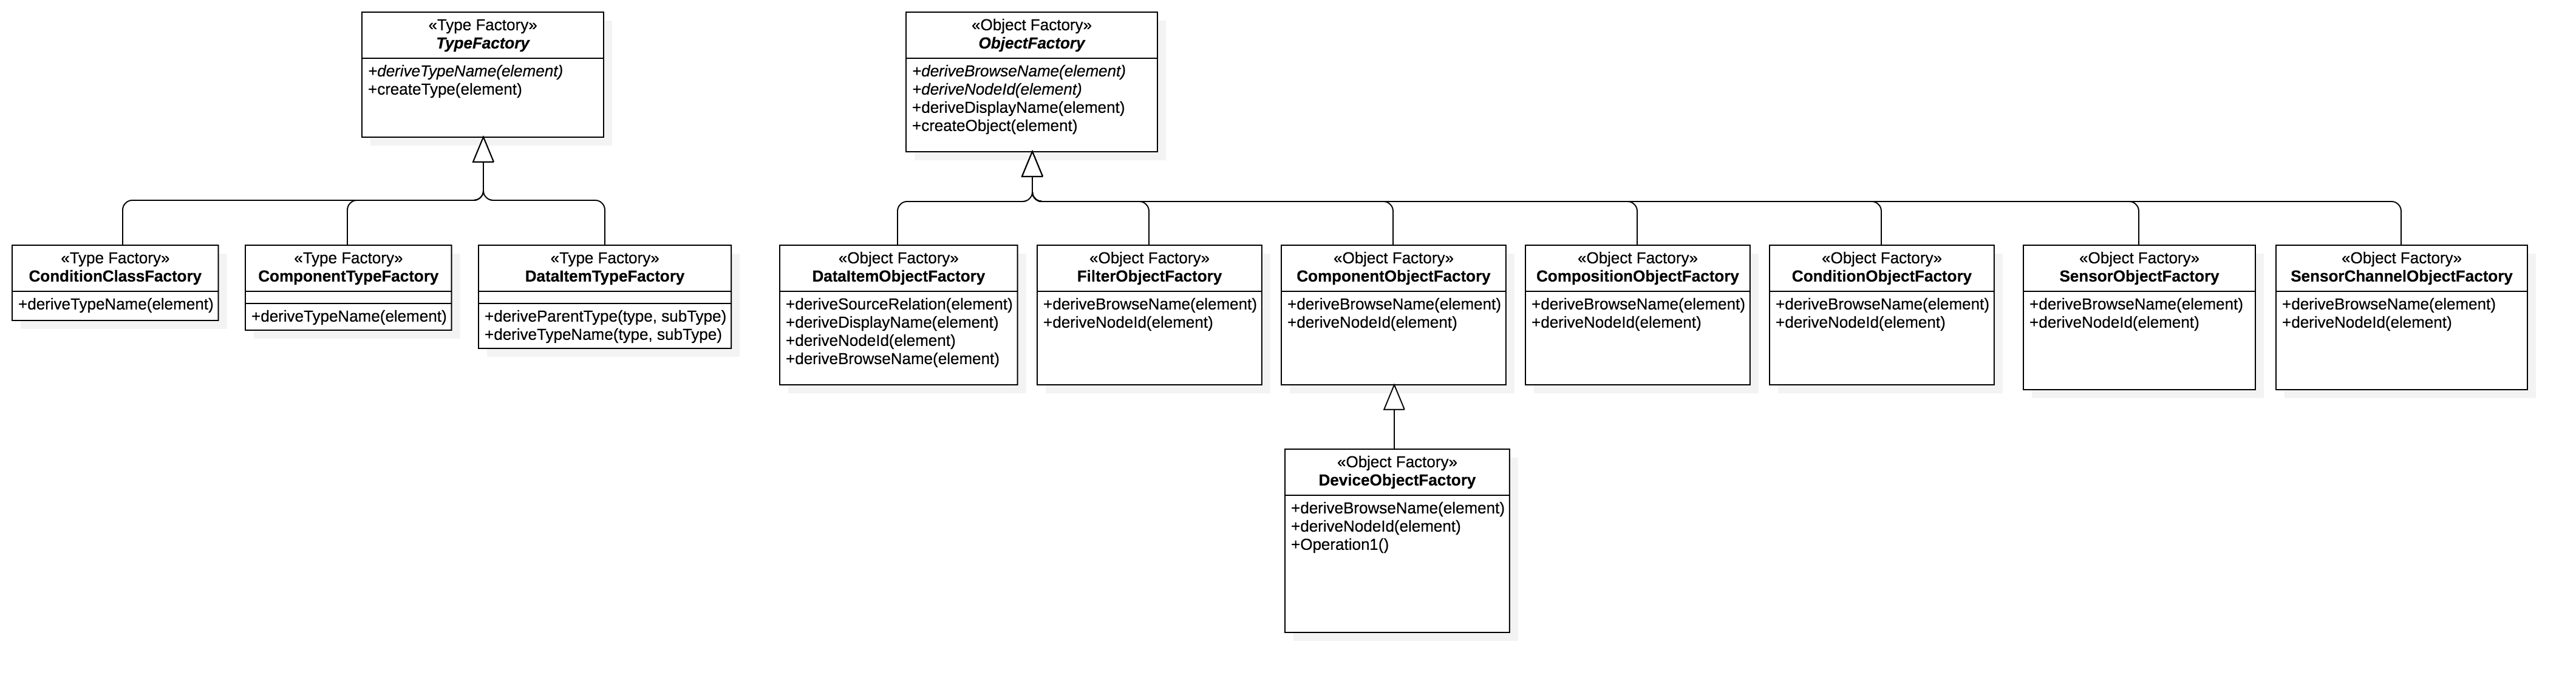
\includegraphics[width=1.0\textwidth]{./diagrams/Factories.png}
  \caption{Factories Diagram}
  \label{fig:Factories}
\end{figure}

\FloatBarrier


\input ./type-sections/Factories.tex

\subsubsection{Defintion of \texttt{<<Object Factory>> ObjectFactory}} \label{type:ObjectFactory}

\FloatBarrier



\paragraph{Operations}
\begin{itemize}
  \item \texttt{deriveBrowseName(element)}
  \item \texttt{deriveNodeId(element)}
  \item \texttt{deriveDisplayName(element)}\\
    Specification:
   \indent \begin{lstlisting}
deriveBrowseName(element)
\end{lstlisting}

  \item \texttt{createObject(element)}
\end{itemize}
\FloatBarrier
\subsubsection{Defintion of \texttt{<<Object Factory>> DataItemObjectFactory}} \label{type:DataItemObjectFactory}

\FloatBarrier



\paragraph{Operations}
\begin{itemize}
  \item \texttt{deriveSourceRelation(element)}
    Documentation: Use the source composition,  component id, or data item id to locate the source node id for this relationship. If one exists, add an object with  browse name "source" that relates to the entity referenced by the id. 

The most specific identity should be used in the following order:
\begin{itemize}
\item \texttt{DataItemId}
\item \texttt{CompositionId}
\item \texttt{ComponentId}
\end{itemize}

Since the data item implies composition and component and the composition implies component, there should only be one attribute given for the source.

  \item \texttt{deriveDisplayName(element)}
    Documentation: Same as the BrowseName.

  \item \texttt{deriveNodeId(element)}
    Documentation: The nodeId will be given by the device uuid and the DataItem id attribute.

  \item \texttt{deriveBrowseName(element)}
    Documentation: The browse name will be composed of the following parts of the model:

\begin{enumerate}
\item If the compositionId is present, the compositionId will be resolved the the Composition element and the pascal case of the type attribute will be placed first.
\item If the subType is present, the pascal case of the subType will be placed next.
\item The pascal case of the type will be placed last.
\end{enumerate}

For example, for a data item with the following attributes:

\begin{itemize}
\item type: \texttt{TEMPERATURE}
\item composition type: \texttt{STORAGE_BATTERY}
\end{itemize}

will have the following browse name: \texttt{StorageBatteryTemperature}

For the data item with the following attributes:

\begin{itemize}
\item type: \texttt{ANGLE}
\item subType: \texttt{ACTUAL}
\item composition type: \texttt{ENCODER}
\end{itemize}

will have the following browse name: \texttt{EncoderActualAngle}


\end{itemize}
\paragraph{Dependency on MTMessageType}

This class relates to \texttt{MTMessageType} (See section \ref{type:MTMessageType}) for a(n) \texttt{Instantiates} relationship.

\paragraph{Dependency on AssetEventType}

This class relates to \texttt{AssetEventType} (See section \ref{type:AssetEventType}) for a(n) \texttt{Instantiates} relationship.

\paragraph{Dependency on MTSampleType}

This class relates to \texttt{MTSampleType} (See section \ref{type:MTSampleType}) for a(n) \texttt{Instantiates} relationship.

\paragraph{Dependency on MTNumericEventType}

This class relates to \texttt{MTNumericEventType} (See section \ref{type:MTNumericEventType}) for a(n) \texttt{Instantiates} relationship.

\paragraph{Dependency on MTEnumeratedEventType}

This class relates to \texttt{MTEnumeratedEventType} (See section \ref{type:MTEnumeratedEventType}) for a(n) \texttt{Instantiates} relationship.

\FloatBarrier
\subsubsection{Defintion of \texttt{<<Object Factory>> FilterObjectFactory}} \label{type:FilterObjectFactory}

\FloatBarrier

Creates filters based on the type attribute of the Filter element. 

\paragraph{Operations}
\begin{itemize}
  \item \texttt{deriveBrowseName(element)}
  \item \texttt{deriveNodeId(element)}
    Documentation: The node id is composed of the data item id and the browse name.

\end{itemize}
\paragraph{Dependency on MinimumDeltaFilterType}

This class relates to \texttt{MinimumDeltaFilterType} (See section \ref{type:MinimumDeltaFilterType}) for a(n) \texttt{Instantiates} relationship.

\paragraph{Dependency on PeriodFilterType}

This class relates to \texttt{PeriodFilterType} (See section \ref{type:PeriodFilterType}) for a(n) \texttt{Instantiates} relationship.

\FloatBarrier
\subsubsection{Defintion of \texttt{<<Object Factory>> ComponentObjectFactory}} \label{type:ComponentObjectFactory}

\FloatBarrier



\paragraph{Operations}
\begin{itemize}
  \item \texttt{deriveBrowseName(element)}\\
    Specification:
   \indent \begin{lstlisting}
concat(element.QName, (if self.name.notEmpty() then concat('[', self.name, ']')) else  '' endif))
\end{lstlisting}

  \item \texttt{deriveNodeId(element)}\\
    Specification:
   \indent \begin{lstlisting}
concat(self.findDevice().uuid, element.id)
\end{lstlisting}

\end{itemize}
\FloatBarrier
\subsubsection{Defintion of \texttt{<<Object Factory>> DeviceObjectFactory}} \label{type:DeviceObjectFactory}

\FloatBarrier

The model instantiation for MTConnect begins with the `Device` MTConnect element and then recursively traverses the sub-elements. The device will the capabilities in the component factory to generate all the data items and component types. 

\paragraph{Operations}
\begin{itemize}
  \item \texttt{deriveBrowseName(element)}\\
    Specification:
   \indent \begin{lstlisting}
derive: element.name
\end{lstlisting}

  \item \texttt{deriveNodeId(element)}\\
    Specification:
   \indent \begin{lstlisting}
derive: element.uuid
\end{lstlisting}

\end{itemize}
\paragraph{Dependency on MTDeviceType}

This class relates to \texttt{MTDeviceType} (See section \ref{type:MTDeviceType}) for a(n) \texttt{Instantiates} relationship.

\FloatBarrier
\subsubsection{Defintion of \texttt{<<Object Factory>> CompositionObjectFactory}} \label{type:CompositionObjectFactory}

\FloatBarrier



\paragraph{Operations}
\begin{itemize}
  \item \texttt{deriveBrowseName(element)}\\
    Specification:
   \indent \begin{lstlisting}
concat(pascalCase(element.type), (if self.name.notEmpty() then concat('[', self.name, ']')) else  '' endif))
\end{lstlisting}

  \item \texttt{deriveNodeId(element)}\\
    Specification:
   \indent \begin{lstlisting}
concat(self.findDevice().uuid, element.id)
\end{lstlisting}

\end{itemize}
\paragraph{Dependency on {Composition}Type}

This class relates to \texttt{{Composition}Type} (See section \ref{type:{Composition}Type}) for a(n) \texttt{Instantiates} relationship.

\FloatBarrier
\subsubsection{Defintion of \texttt{<<Object Factory>> ConditionObjectFactory}} \label{type:ConditionObjectFactory}

\FloatBarrier



\paragraph{Operations}
\begin{itemize}
  \item \texttt{deriveBrowseName(element)}
  \item \texttt{deriveNodeId(element)}
\end{itemize}
\paragraph{Dependency on MTExclusiveLimitConditionType}

This class relates to \texttt{MTExclusiveLimitConditionType} (See section \ref{type:MTExclusiveLimitConditionType}) for a(n) \texttt{Instantiates} relationship.

\paragraph{Dependency on MTNonExclusiveConditionType}

This class relates to \texttt{MTNonExclusiveConditionType} (See section \ref{type:MTNonExclusiveConditionType}) for a(n) \texttt{Instantiates} relationship.

\FloatBarrier
\subsubsection{Defintion of \texttt{<<Object Factory>> SensorObjectFactory}} \label{type:SensorObjectFactory}

\FloatBarrier



\paragraph{Operations}
\begin{itemize}
  \item \texttt{deriveBrowseName(element)}\\
    Specification:
   \indent \begin{lstlisting}
element.QName
\end{lstlisting}

  \item \texttt{deriveNodeId(element)}\\
    Specification:
   \indent \begin{lstlisting}
concat(self.parent.NodeId, BrowseName)
\end{lstlisting}

\end{itemize}
\paragraph{Dependency on SensorConfigurationType}

This class relates to \texttt{SensorConfigurationType} (See section \ref{type:SensorConfigurationType}) for a(n) \texttt{Instantiates} relationship.

\FloatBarrier
\subsubsection{Defintion of \texttt{<<Object Factory>> SensorChannelObjectFactory}} \label{type:SensorChannelObjectFactory}

\FloatBarrier



\paragraph{Operations}
\begin{itemize}
  \item \texttt{deriveBrowseName(element)}\\
    Specification:
   \indent \begin{lstlisting}
concat('Channel', self.number)
\end{lstlisting}

  \item \texttt{deriveNodeId(element)}\\
    Specification:
   \indent \begin{lstlisting}
concat(self.parent.NodeId, BrowseName)
\end{lstlisting}

\end{itemize}
\paragraph{Dependency on ChannelType}

This class relates to \texttt{ChannelType} (See section \ref{type:ChannelType}) for a(n) \texttt{Instantiates} relationship.

\FloatBarrier
\subsubsection{Defintion of \texttt{<<Type Factory>> TypeFactory}} \label{type:TypeFactory}

\FloatBarrier



\paragraph{Operations}
\begin{itemize}
  \item \texttt{deriveTypeName(element)}
  \item \texttt{createType(element)}
\end{itemize}
\FloatBarrier
\subsubsection{Defintion of \texttt{<<Type Factory>> ComponentTypeFactory}} \label{type:ComponentTypeFactory}

\FloatBarrier

The \texttt{ComponentTypeFactory} creates component types using the MTConnect XML element as an input. 
The factory takes the \texttt{QName} (or qualified name) of the XML element and then appends \texttt{Type}. For 
example an \texttt{<Controller id='...'></...>} element will create an OPC/UA `ControllerType` type definition 
as an extension of the base \texttt{MTControllerType}. 

Currently there is no additional abstractions or super types required by the companion specification. 
The types will be a single level where each Component is a sub-type of the base \texttt{MTComponentType}.


\paragraph{Operations}
\begin{itemize}
  \item \texttt{deriveTypeName(element)}\\
    Specification:
   \indent \begin{lstlisting}
derive: Component <- element.QName
\end{lstlisting}

    Documentation: The QName of the element for the component will be used to derive the type of the node.

\end{itemize}
\paragraph{Dependency on {Component}Type}

This class relates to \texttt{{Component}Type} (See section \ref{type:{Component}Type}) for a(n) \texttt{Instantiates} relationship.

\FloatBarrier
\subsubsection{Defintion of \texttt{<<Type Factory>> CompositionTypeFactory}} \label{type:CompositionTypeFactory}

\FloatBarrier



\paragraph{Operations}
\begin{itemize}
  \item \texttt{deriveTypeName(element)}\\
    Specification:
   \indent \begin{lstlisting}
derive: Composition <-
 pascalCase(element.type)
\end{lstlisting}

    Documentation: The type for the composition will be created using the pascal case of the \texttt{type} from the composition element.

\end{itemize}
\FloatBarrier
\subsection{MTConnect Device Profile} \label{model:MTConnectDeviceProfile}

\begin{figure}[ht]
  \centering
    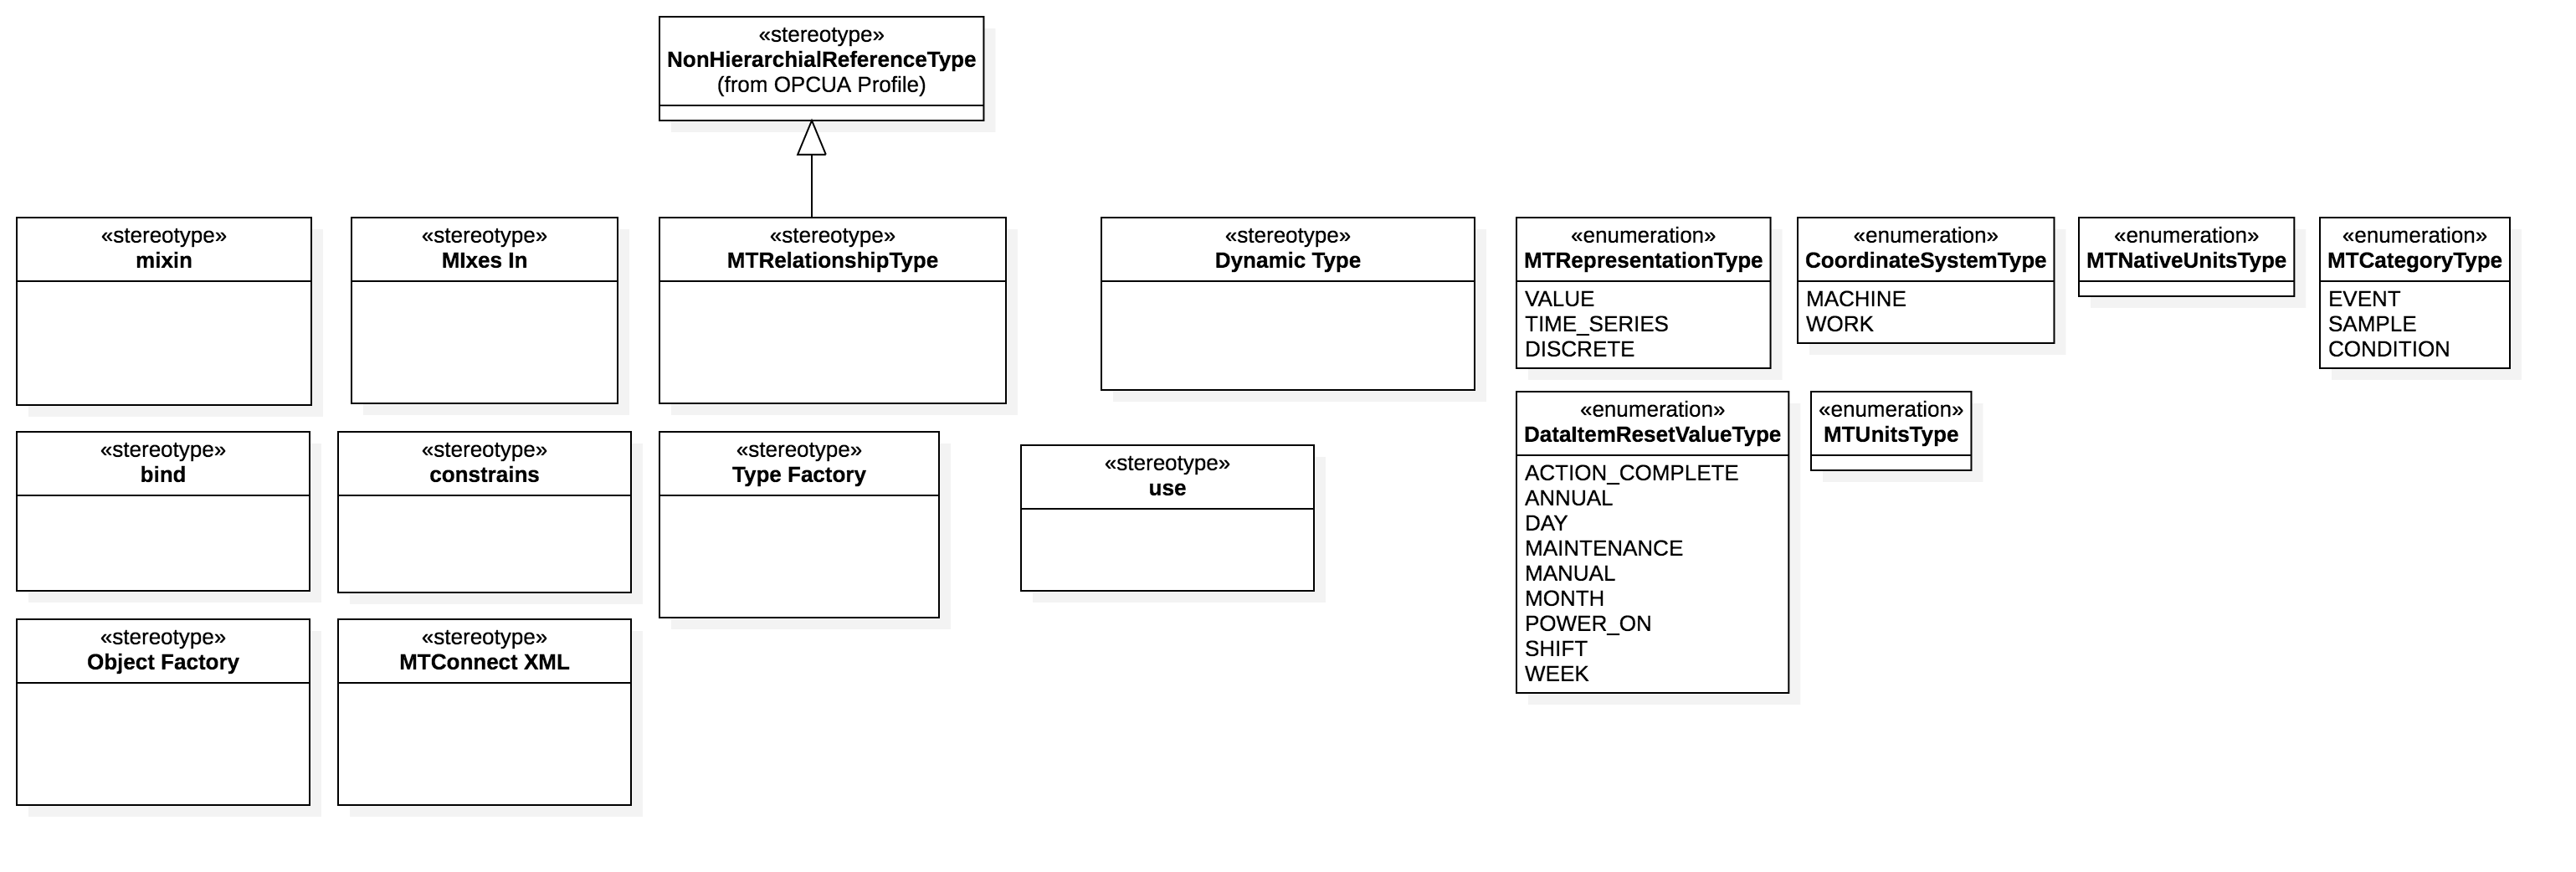
\includegraphics[width=1.0\textwidth]{./diagrams/MTConnectDeviceProfile.png}
  \caption{MTConnect Device Profile Diagram}
  \label{fig:MTConnectDeviceProfile}
\end{figure}

\FloatBarrier


The device profile documents the common data types and stereotypes that are 
used to construct the model. A stereotype is a design or modeling pattern that 
provides additional information about the type or the relationship between types. 

It can also identify the behavior of a property or the role the type or relation
will play in the model. 

Stereotypes are used throughout the model to provide additional information that 
will halp provide context and definition to aid in better understanding the
data model.

\subsubsection{Defintion of \texttt{ Dynamic Type}} \label{type:Dynamic Type}

\FloatBarrier

A dynamic type indicates that the class browse name and type will be 
determined at configuration time based on the MTConnect \texttt{Device}
elements.

\FloatBarrier
\subsubsection{Defintion of \texttt{ HasChannels}} \label{type:HasChannels}

\FloatBarrier

The relationship type for the MTConnect \texttt{SensorConfiguration} set of 
associate \texttt{Channels}.

\begin{table}[ht]
\centering 
  \caption{\texttt{HasChannels} Definition}
  \label{table:HasChannels}
\fontsize{9pt}{11pt}\selectfont
\tabulinesep=3pt
\begin{tabu} to 6in {|l|l|l|l|l|l|} \everyrow{\hline}
\hline
\rowfont\bfseries {Attribute} & \multicolumn{5}{|l|}{Value} \\
\tabucline[1.5pt]{}
BrowseName & \multicolumn{5}{|l|}{HasChannels} \\
IsAbstract & \multicolumn{5}{|l|}{False} \\
Symmetric & \multicolumn{5}{|l|}{false} \\
\tabucline[1.5pt]{}
\rowfont \bfseries References & NodeClass & BrowseName & DataType & TypeDefinition & {Modeling Rule} \\
\multicolumn{6}{|l|}{Subtype of \texttt{Aggregates} (See OPCUA Profile Documentation)} \\
\end{tabu}
\end{table} 


\FloatBarrier
\subsubsection{Defintion of \texttt{ HasMTClassType}} \label{type:HasMTClassType}

\FloatBarrier



\begin{table}[ht]
\centering 
  \caption{\texttt{HasMTClassType} Definition}
  \label{table:HasMTClassType}
\fontsize{9pt}{11pt}\selectfont
\tabulinesep=3pt
\begin{tabu} to 6in {|l|l|l|l|l|l|} \everyrow{\hline}
\hline
\rowfont\bfseries {Attribute} & \multicolumn{5}{|l|}{Value} \\
\tabucline[1.5pt]{}
BrowseName & \multicolumn{5}{|l|}{HasMTClassType} \\
IsAbstract & \multicolumn{5}{|l|}{False} \\
Symmetric & \multicolumn{5}{|l|}{false} \\
\tabucline[1.5pt]{}
\rowfont \bfseries References & NodeClass & BrowseName & DataType & TypeDefinition & {Modeling Rule} \\
\multicolumn{6}{|l|}{Subtype of \texttt{NonHierarchialReferenceType} (See OPCUA Profile Documentation)} \\
\end{tabu}
\end{table} 


\FloatBarrier
\subsubsection{Defintion of \texttt{ HasMTComposition}} \label{type:HasMTComposition}

\FloatBarrier



\begin{table}[ht]
\centering 
  \caption{\texttt{HasMTComposition} Definition}
  \label{table:HasMTComposition}
\fontsize{9pt}{11pt}\selectfont
\tabulinesep=3pt
\begin{tabu} to 6in {|l|l|l|l|l|l|} \everyrow{\hline}
\hline
\rowfont\bfseries {Attribute} & \multicolumn{5}{|l|}{Value} \\
\tabucline[1.5pt]{}
BrowseName & \multicolumn{5}{|l|}{HasMTComposition} \\
IsAbstract & \multicolumn{5}{|l|}{False} \\
Symmetric & \multicolumn{5}{|l|}{false} \\
\tabucline[1.5pt]{}
\rowfont \bfseries References & NodeClass & BrowseName & DataType & TypeDefinition & {Modeling Rule} \\
\multicolumn{6}{|l|}{Subtype of \texttt{Organizes} (See OPCUA Profile Documentation)} \\
\end{tabu}
\end{table} 


\FloatBarrier
\subsubsection{Defintion of \texttt{ HasMTCondition}} \label{type:HasMTCondition}

\FloatBarrier

The relationship associated with the collection of MTConnect \texttt{Conditions} associated with
the MTConnect \texttt{Component}

\begin{table}[ht]
\centering 
  \caption{\texttt{HasMTCondition} Definition}
  \label{table:HasMTCondition}
\fontsize{9pt}{11pt}\selectfont
\tabulinesep=3pt
\begin{tabu} to 6in {|l|l|l|l|l|l|} \everyrow{\hline}
\hline
\rowfont\bfseries {Attribute} & \multicolumn{5}{|l|}{Value} \\
\tabucline[1.5pt]{}
BrowseName & \multicolumn{5}{|l|}{HasMTCondition} \\
IsAbstract & \multicolumn{5}{|l|}{False} \\
Symmetric & \multicolumn{5}{|l|}{false} \\
\tabucline[1.5pt]{}
\rowfont \bfseries References & NodeClass & BrowseName & DataType & TypeDefinition & {Modeling Rule} \\
\multicolumn{6}{|l|}{Subtype of \texttt{Organizes} (See OPCUA Profile Documentation)} \\
\end{tabu}
\end{table} 


\FloatBarrier
\subsubsection{Defintion of \texttt{ HasMTReferenceType}} \label{type:HasMTReferenceType}

\FloatBarrier



\begin{table}[ht]
\centering 
  \caption{\texttt{HasMTReferenceType} Definition}
  \label{table:HasMTReferenceType}
\fontsize{9pt}{11pt}\selectfont
\tabulinesep=3pt
\begin{tabu} to 6in {|l|l|l|l|l|l|} \everyrow{\hline}
\hline
\rowfont\bfseries {Attribute} & \multicolumn{5}{|l|}{Value} \\
\tabucline[1.5pt]{}
BrowseName & \multicolumn{5}{|l|}{HasMTReferenceType} \\
IsAbstract & \multicolumn{5}{|l|}{False} \\
Symmetric & \multicolumn{5}{|l|}{false} \\
\tabucline[1.5pt]{}
\rowfont \bfseries References & NodeClass & BrowseName & DataType & TypeDefinition & {Modeling Rule} \\
\multicolumn{6}{|l|}{Subtype of \texttt{HasComponent} (See OPCUA Profile Documentation)} \\
\end{tabu}
\end{table} 


\FloatBarrier
\subsubsection{Defintion of \texttt{ HasMTSubClassType}} \label{type:HasMTSubClassType}

\FloatBarrier



\begin{table}[ht]
\centering 
  \caption{\texttt{HasMTSubClassType} Definition}
  \label{table:HasMTSubClassType}
\fontsize{9pt}{11pt}\selectfont
\tabulinesep=3pt
\begin{tabu} to 6in {|l|l|l|l|l|l|} \everyrow{\hline}
\hline
\rowfont\bfseries {Attribute} & \multicolumn{5}{|l|}{Value} \\
\tabucline[1.5pt]{}
BrowseName & \multicolumn{5}{|l|}{HasMTSubClassType} \\
IsAbstract & \multicolumn{5}{|l|}{False} \\
Symmetric & \multicolumn{5}{|l|}{false} \\
\tabucline[1.5pt]{}
\rowfont \bfseries References & NodeClass & BrowseName & DataType & TypeDefinition & {Modeling Rule} \\
\multicolumn{6}{|l|}{Subtype of \texttt{NonHierarchialReferenceType} (See OPCUA Profile Documentation)} \\
\end{tabu}
\end{table} 


\FloatBarrier
\subsubsection{Defintion of \texttt{ MTComponentReference}} \label{type:MTComponentReference}

\FloatBarrier



\FloatBarrier
\subsubsection{Defintion of \texttt{ MTConnect XML}} \label{type:MTConnect XML}

\FloatBarrier



\FloatBarrier
\subsubsection{Defintion of \texttt{ Mixes In}} \label{type:Mixes In}

\FloatBarrier

This stereotype is associated with the dependency between a type and a mixin. See Section \ref{type:mixin} for a complete 
description of the mixin.

\FloatBarrier
\subsubsection{Defintion of \texttt{ Object Factory}} \label{type:Object Factory}

\FloatBarrier



\FloatBarrier
\subsubsection{Defintion of \texttt{<<Type Factory>> Type Factory}} \label{type:Type Factory}

\FloatBarrier



\FloatBarrier
\subsubsection{Defintion of \texttt{ bind}} \label{type:bind}

\FloatBarrier

When a dynamic type (See Section \ref{type:Dynamic Type}) creates an instance where the super-type
can be associated based on the data item category and type, the \texttt{Type Factory} will 
specify which supertype is to be referenced.

The \texttt{bind} stereotype indicates the relationship between the dynamic sub-type and the 
parent type are resolved based on the MTConnect DataItem meta data.

\FloatBarrier
\subsubsection{Defintion of \texttt{ constrains}} \label{type:constrains}

\FloatBarrier



\FloatBarrier
\subsubsection{Defintion of \texttt{ data type}} \label{type:data type}

\FloatBarrier

Represents a relationship between a Variable and the data type.

\FloatBarrier
\subsubsection{Defintion of \texttt{ event}} \label{type:event}

\FloatBarrier

In the object model, represents Variables that are of the MTConnect \texttt{Event} category.

\FloatBarrier
\subsubsection{Defintion of \texttt{ mixin}} \label{type:mixin}

\FloatBarrier

The mixin pattern injects the properties and operations into the types 
that are related to the using the \texttt{Mixes In} dependency. Mixins allow for
lightweight multiple inheritance. Since OPC/UA does not allow for multiple inheritance 
and the MTConnect  types require the same set of properties when they are sub-typed
from existing OPC/UA types, this mechanism allows for this relationship to be expressed.


\FloatBarrier
\subsubsection{Defintion of \texttt{ sample}} \label{type:sample}

\FloatBarrier

In the object model, represents Variables that are of the MTConnect \texttt{Sample} category.

\FloatBarrier
\subsubsection{Defintion of \texttt{ use}} \label{type:use}

\FloatBarrier

The use stereotype indicates that one class uses another as a helper to perform 
a specific operation or activity. This stereotype is mainly used to indicate
that a specific factory is being employed by another type to create dynamic
properties or relationships.

\FloatBarrier
\subsubsection{Defintion of \texttt{ values}} \label{type:values}

\FloatBarrier

For controlled vocabularies of enumerated types, specifies the relationship to the allowable 
values for the type.

\FloatBarrier
